\documentclass[11pt]{article}
\usepackage[super,sort&compress,comma]{natbib} 
%\usepackage{natbib}
\usepackage[version=3]{mhchem}
\usepackage[left=2.3cm, right=3cm, top=1.785cm, bottom=2.0cm]{geometry}
\usepackage{graphicx} 
\usepackage[format=plain,justification=justified,singlelinecheck=false,font={stretch=1.125,sf},labelfont=bf,labelsep=space]{caption}
\usepackage[english]{babel}
\usepackage[T1]{fontenc}
\usepackage[dvipsnames]{xcolor}
\usepackage{setspace}
\usepackage{hyperref}
\usepackage{threeparttable}
\usepackage{tablefootnote}
\usepackage{longtable}
\usepackage{hhline}
\usepackage{booktabs}
\usepackage{multirow}
\usepackage{array}
\usepackage{multicol,caption,listings}
\usepackage{authblk}
\usepackage{float} 
\usepackage{pgfplots}
\usepgfplotslibrary{groupplots}
\pgfplotsset{compat=1.18}

\usepackage{siunitx}
\DeclareSIUnit\angstromunit{\text{\AA}}
\sisetup{
  round-mode = places,
  %round-precision = 7
}

%%::::::::::::::: COLOR TEXT:::::::::::::::::::::::::::::::::::::
\newcommand{\itblue}[1]{\textcolor{blue}{\textit{#1}}}
\newcommand{\blue}[1]{{\color{blue}#1\color{black}}}
\newcommand{\red}[1]{{\color{red}#1\color{black}}}

%HIDE column
\newcolumntype{H}{>{\setbox0=\hbox\bgroup}c<{\egroup}@{}}

\onehalfspacing{}

\newlength\Colsep
\setlength\Colsep{10pt}
\newcommand{\txe}[1]{{\color{red}#1\color{black}}}
\hyphenation{con-tri-bu-tion con-fi-gu-ra-tion
ex-pe-ri-men-tal me-a-su-ra-ble a-vo-ga-dro}
%%:::::::::::::::::::::::::::::::::::::::::::::::::::::::::::::::
%%::::::::::::    BEGIN DOCUMENT    :::::::::::::::::::::::::::::
%%:::::::::::::::::::::::::::::::::::::::::::::::::::::::::::::::

%\author{Rafael Grande-Aztatzi$^{*}$, , Jesus M. Ugalde and Jose M. Mercero$^{*}$}

%
\title{Composition and Structural Effects on CO Binding in \ce{Pt10} and Pt--Ge Clusters}

\author[1,2,3]{Andoni Ugartemendia}
%\author[1,2]{Sílvia Escayola}
\author[1,2]{Idoia}
\author[1,2]{Ramon}
\author[1,2,$^*$]{Elisa Jimenez-Izal}
\author[1,2,$^*$]{Jose M. Mercero }
\affil[1]{\small Donostia International Physics Center (DIPC), 20018 Donostia, Euskadi, Spain}
\affil[2]{\small Kimika Fakultatea, Euskal Herriko Unibertsitatea (UPV/EHU), P.K. 1072, 20080 Donostia, Euskadi, Spain}
%\affil[4]{\small IKERBASQUE, Basque Foundation for Science, 48013 Bilbao, Euskadi, Spain}
%\affil[5]{\small  Escuela de Ingeniería y Ciencias, Tecnológico de Monterrey, Av. Eugenio Garza Sada 2501, 64849 Monterrey, Nuevo León, México.}


\graphicspath{{Figures/}}

\begin{document}	
\maketitle

%\section{Abstract}
\begin{abstract}
Carbon monoxide binds strongly to platinum and can deactivate Pt-based
catalysts. Ge incorporation can weaken this interaction, but it also changes
the geometry and bonding pattern of small Pt--Ge clusters. We use ten-atom
\ce{Pt10}, \ce{Pt6Ge4}, \ce{Pt5Ge5}, and
\ce{Pt4Ge6} models to examine how these structural and electronic effects act
together.

The main comparison is based on crossed-parent models. In one route, Ge atoms
are introduced into a common \ce{Pt10} framework; in the reverse route, a
\ce{Pt5Ge5} framework is converted into a pure \ce{Pt10} derivative. Within
the common \ce{Pt10}-parent series, the mean binding energy becomes less
negative as the Ge content increases. AdNDP shows a change from delocalized
multicenter bonding in pure \ce{Pt10} to more localized Pt--Ge bonding in the
Ge-containing models. {Calculations with \ce{CO} placed at every
independent Pt site show that the affinity of an individual site depends on the
local environment, parent geometry, and cluster reorganization. Calculations
initiated from previously reported global-minimum structures further show that
the adsorption landscape changes with the parent isomer and spin state.
Overall, increasing the Ge content weakens mean \ce{CO} adsorption within the
crossed-parent series. Individual binding energies vary with the local
environment and with the structural response of the cluster after \ce{CO}
adsorption.}
\end{abstract}


\section{Introduction}
Transition-metal clusters offer useful models for examining how composition,
geometry, spin state, and local coordination influence adsorption at catalytic
metal sites. Their finite size gives access to atom-specific environments that
are difficult to isolate on extended surfaces, while still retaining key
features of heterogeneous catalysts such as low coordination, structural
fluxionality, and strong coupling between geometry and electronic structure.
Platinum-based materials are particularly relevant in this context because of
their high activity in fuel-cell-related processes and in a wide range of
catalytic reactions.\cite{jimenezizal:2018,jimenezizal:2019b,yu:2002,
zhang:2014,auer:1998} This performance, however, comes with a well-known
limitation, since Pt binds carbon monoxide strongly. Even small amounts of \ce{CO}
can block Pt active sites and cause severe deactivation, especially in
fuel-cell environments.\cite{cheng:2007,vogel:1975,baschuk:2001,
christoffersen:2001,yang:2021} Alloying Pt with a second element is therefore
a common strategy to tune the electronic structure of the active sites, reduce
Pt loading, and mitigate \ce{CO} poisoning.\cite{yousaf:2016,yin:2011,
stolbov:2009,lee:1999,hayden:2003,samjeske:2002,ferrari:2016,ahmad:2015,
ehteshami:2013,chen:2019,ribeiro:2019}

Germanium has emerged as a particularly interesting promoter for Pt. Pt--Ge
materials have been reported to improve activity or durability in hydrogen
evolution, direct methanol fuel cells, \ce{CO} oxidation, dehydrogenation, and
reforming reactions, with the Ge component modifying both the structure and the
electronic properties of the Pt sites.\cite{lim:2018,veizaga:2014,
veizaga:2019,crabb:2001,gyorffy:2009,poths:2023,vilella:2008,rimaz:2019,
jimenezizal:2019,ma:2023,garetto:1996,mazzieri:2009,mariscal:2007}
Experimental and theoretical studies on \ce{PtGe/C} electrocatalysts have also
shown modified \ce{CO} oxidation behavior relative to monometallic Pt
systems.\cite{veizaga:2014,veizaga:2019,crabb:2001} These observations suggest
that Ge can act through both geometric effects, by disrupting contiguous Pt
ensembles, and electronic effects, by changing the electron density and orbital
availability at Pt.
Experiments on \ce{Pt(111)-Ge} surface alloys also reported weaker \ce{CO}
chemisorption than on \ce{Pt(111)} and associated this change with the modified
electronic structure of Pt after Ge incorporation.\cite{fukutani:1996,fukutani:1998}
Earlier calculations on Pt--Ge cluster models likewise found weaker Pt--C
interactions and changes in the \ce{C-O} stretching frequency after Ge
substitution.\cite{liao:2000}

Gas-phase and supported clusters provide a controlled route to examine these
effects in atomically defined environments. A recent review of \ce{CO}
adsorption on doped metal clusters emphasizes the coupled roles of composition,
charge state, and local environment.\cite{ferrari:2020} For 13-atom Pt--Au
clusters, Morrow and co-workers showed that the local environment of the
adsorption atom affects both the \ce{CO} binding energy and stretching
frequency.\cite{morrow:2011} Ugartemendia and co-workers combined density
functional theory (DFT)
with mass spectrometry to study \ce{Pt_n^+} and \ce{GePt_{n-1}^+} clusters
with $n=5$--9.\cite{ugartemendia:2021} Their global-minimum searches and
electronic-structure analyses showed that replacing one Pt atom by Ge generally
weakens the Pt--CO interaction while the clusters remain active toward
\ce{H2} dissociation. Within a Blyholder-type interpretation, the weaker
{\ce{CO} binding was assigned mainly to reduced Pt $\rightarrow$ \ce{CO}
$\pi$ back-donation. In this interpretation, Pt--Ge orbital mixing competes
with the Pt orbitals that would otherwise interact with the \ce{CO} $2\pi^*$
acceptor manifold.}

A subsequent study extended this idea from monodoped cationic clusters to
\ce{Pt_{n-m}Ge_m} nanoclusters with different sizes and
compositions.\cite{ugartemendia:2022} {That work found especially weak
\ce{CO} binding and high resistance to poisoning in clusters with roughly
equimolar Pt:Ge ratios. The authors traced this behavior to strong Pt--Ge
covalency and electrostatic stabilization from favorable Pt--Ge mixing.} In
the same work, AdNDP analysis revealed a
clear bonding contrast between pure and equimolar clusters. Pure \ce{Pt10}
was described by delocalized multicenter Pt bonding, whereas \ce{Pt5Ge5}
could be represented mainly by localized Pt--Ge two-center bonds. {This
contrast suggests that weaker \ce{CO} adsorption may depend on the Ge content
and on how Ge changes the bonding framework around the Pt adsorption site.}

More recent work on supported \ce{PtGe} clusters has reinforced this picture
while adding the role of the support and reaction environment. Deposited
\ce{Pt4Ge_n} clusters on MgO were proposed to operate as bifunctional
catalysts for \ce{CO} oxidation, with \ce{CO} binding preferentially at Pt and
oxygen binding at Ge-derived sites; at the same time, Ge alloying reduces the
affinity of Pt for \ce{CO} and relieves self-poisoning.\cite{ugartemendia:2024}
Related studies in alkane dehydrogenation further indicate that the Pt:Ge ratio
can control activity, selectivity, coke resistance, and sintering resistance in
supported Pt--Ge clusters.\cite{poths:2023b} Taken together, these studies show
that Ge is not a passive diluent. It changes the local chemistry of Pt, the
stability of the cluster, and the possible reaction pathways available under
catalytic conditions.

The present work examines ten-atom \ce{Pt10}, \ce{Pt_{x}Ge_{10-x}}, (where x=4,5,6),
clusters using DFT\@. The study uses two crossed
construction routes. In the first, we start from the previously reported
lowest-energy, or global-minimum (GM), \ce{Pt10} framework and replace selected
Pt atoms by Ge. In the reverse route, we start from the previously reported GM
\ce{Pt5Ge5} framework and replace all Ge atoms by Pt, producing a pure-
\ce{Pt10} derivative.\cite{ugartemendia:2022} The resulting structures provide
selected comparisons of composition and starting geometry within related
ten-atom frameworks.

\ce{CO} is then placed in turn at each independent Pt environment represented
in these parent structures, and each structure is fully optimized. This
procedure shows how the binding energy depends on composition, parent geometry,
spin state, local bonding, and relaxation of the whole cluster. In addition, we
start separate calculations from the reported global-minimum structure of each
composition. Comparing the two sets shows whether the adsorption pattern changes
when a different parent structure or spin state is used.

\section{Methods}
All cluster calculations were performed with Gaussian~16\cite{g16}
using the PBE exchange--correlation functional (PBEPBE).\cite{perdew:pbe:1996}
A def2-TZVP basis was used for C, O, and Ge,\cite{weigend:def2:2005}
and Pt was described with the corresponding Karlsruhe valence basis and a
60-electron \textcolor{cyan}{scalar relativistic} effective core potential \textcolor{cyan}{(ECP)}.\cite{andrae:epp:1990,weigend:def2:2005}
This leaves 18 explicit Pt electrons.
Geometry optimizations and harmonic
frequency calculations were carried out for the bare clusters, carbonyl
complexes, and free \ce{CO}. All structures in the adsorption
analysis were confirmed as true minima by the absence of imaginary frequencies.
Orbital stability was tested for the selected triplet
\ce{Pt10} solution and for the seven distinct triplet \ce{Pt10CO} minima
obtained after placing \ce{CO} at independent Pt sites.
All these wavefunctions were stable under the
perturbations considered.

The structural families used in the adsorption study are summarized in
Figure~\ref{fig:neutral_data_sets}. For the crossed-parent models, the spin
states were optimized separately before \ce{CO} adsorption was considered.
The \ce{Pt6Ge4}, \ce{Pt5Ge5}, and \ce{Pt4Ge6} structures were generated from
the reported global-minimum \ce{Pt10} framework.\cite{ugartemendia:2022} In the reverse route, the
triplet \ce{Pt10} structure was generated from the reported global-minimum
\ce{Pt5Ge5} framework. The reported global-minimum structure of each
composition was also reoptimized at the same level and used in a separate
comparison set.

\begin{figure}[H]
\centering
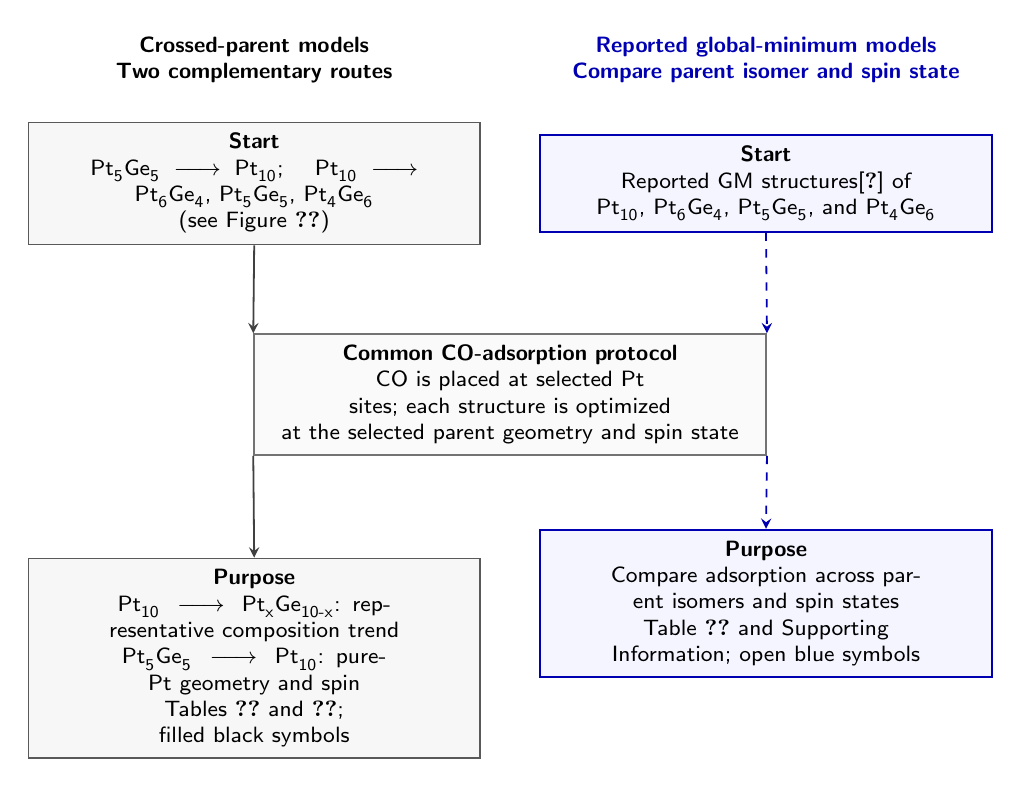
\begin{tikzpicture}[
  x=1cm,
  y=1cm,
  header/.style={font=\sffamily\bfseries\footnotesize, align=center},
  crossbox/.style={draw=black!65, line width=0.65pt, fill=black!3,
    text width=5.45cm, align=center, inner sep=4pt,
    font=\sffamily\footnotesize},
  gmbox/.style={draw=blue!70!black, line width=0.65pt, fill=blue!4,
    text width=5.45cm, align=center, inner sep=4pt,
    font=\sffamily\footnotesize},
  commonbox/.style={draw=black!55, line width=0.65pt, fill=black!2,
    text width=6.22cm, align=center, inner sep=4pt,
    font=\sffamily\footnotesize},
  crossarrow/.style={->, >=stealth, line width=0.65pt, black!75},
  gmarrow/.style={->, >=stealth, line width=0.65pt, blue!70!black, dashed}
]

\node[header] at (-3.25,2.25)
  {Crossed-parent models\\Two complementary routes};
\node[header,text=blue!70!black] at (3.25,2.25)
  {Reported global-minimum models\\Compare parent isomer and spin state};

\node[crossbox] (crossedstart) at (-3.25,0.68)
  {\textbf{Start}\\
   \ce{Pt5Ge5 -> Pt10}; \quad
   \ce{Pt10 -> Pt6Ge4}, \ce{Pt5Ge5}, \ce{Pt4Ge6}\\
   (see Figure~\ref{fig:tfg_crossed_models})};
\node[gmbox] (gmstart) at (3.25,0.68)
  {\textbf{Start}\\
   Reported GM structures\cite{ugartemendia:2022} of \ce{Pt10},
   \ce{Pt6Ge4}, \ce{Pt5Ge5}, and \ce{Pt4Ge6}};

\node[commonbox] (adsorption) at (0,-2.0)
  {\textbf{Common \ce{CO}-adsorption protocol}\\
   \ce{CO} is placed at selected Pt sites; each structure is optimized\\
   at the selected parent geometry and spin state};

\node[crossbox] (crosseduse) at (-3.25,-5.35)
  {\textbf{Purpose}\\
   \ce{Pt10 -> Pt_xGe_{10-x}}: representative composition trend\\
   \ce{Pt5Ge5 -> Pt10}: pure-Pt geometry and spin\\
   Tables~\ref{tab:tfg_adsorption_descriptors}
   and~\ref{tab:tfg_bimetallic_adsorption_descriptors};\\
   filled black symbols};
\node[gmbox] (gmuse) at (3.25,-4.65)
  {\textbf{Purpose}\\
   Compare adsorption across parent isomers and spin states\\
   Table~\ref{tab:tfg_adsorption_descriptors} and Supporting\\
   Information; open blue symbols};

\draw[crossarrow] (crossedstart.south) -- (adsorption.north west);
\draw[gmarrow] (gmstart.south) -- (adsorption.north east);
\draw[crossarrow] (adsorption.south west) -- (crosseduse.north);
\draw[gmarrow] (adsorption.south east) -- (gmuse.north);
\end{tikzpicture}

\caption{Organization of the two cluster data sets used for the
\ce{CO}-adsorption analysis. The crossed-parent set contains the
\ce{Pt10}-to-\ce{Pt_{x}Ge_{10-x}} composition sequence and the reverse
\ce{Pt5Ge5}-to-\ce{Pt10} route. Calculations initiated from the reported
global-minimum structures show how the results change with the parent isomer
and spin state. Both sets follow the same adsorption protocol.}
\label{fig:neutral_data_sets}
\end{figure}

For this DFT series, the reported relative energies and \ce{CO}
binding energies include the harmonic zero-point vibrational energy (ZPVE).
Hereafter, ``carbonyl'' denotes the optimized cluster--\ce{CO} complex. We define
\begin{align}
E_0(X) &= E_{\rm elec}(X)+\mathrm{ZPVE}(X),\\
BE(\ce{CO}) &= E_0(\mathrm{carbonyl})
              -E_0(\mathrm{bare\ cluster})-E_0(\ce{CO}).
\label{eq:neutral_dft_be}
\end{align}
Thus, more negative values correspond to stronger adsorption.
Unless stated otherwise, each binding energy is referenced to free singlet
\ce{CO} and to the optimized bare cluster with the same parent framework and
multiplicity as the corresponding carbonyl.

The bonding patterns were analyzed with the adaptive natural density partitioning tool (AdNDP~2.0).\cite{tkachenko:adndp2:2019}
AdNDP searches included the chemically active valence space, with 10
electrons per Pt atom and four per Ge atom. The Pt 5s and 5p semicore orbitals
retained by the ECP were treated as core orbitals.
For the triplet \ce{Pt10}, the $\alpha$ and $\beta$ density matrices were analyzed
independently. Elements involving the same atomic centers in both spin
channels were paired when possible. The Occupation Numbers (ON) indicate the probability of finding two electrons in a given bond. The spin-resolved elements and their
ON are reported in Supporting
Table~\ref{tab:tfg_adndp_summary}.

For selected strongly and weakly bound carbonyl minima of \ce{Pt10},
\ce{Pt6Ge4}, \ce{Pt5Ge5}, and \ce{Pt4Ge6}, interaction and
fragment-reorganization terms were evaluated from electronic single-point
energies. The bare-cluster and \ce{CO} fragments were calculated both in their
isolated optimized geometries and at the coordinates they adopt in the
optimized carbonyl complex. The ZPVE correction was added only after this
electronic decomposition, to obtain the final binding energy.



\section{Results and discussion}

\textbf{AQUI EMPEZARIA EXPLICANDO COMO ES LA GEOMETRIA Y SPIN STATE DE Pt10 Y Pt5Ge5 ORIGINALES Y COMO CAMBIA EN LOS DERIVADOS A RAIZ DE CAMBIAR LA COMPOSICION}

\textbf{GALDERA: AL CAMBIAR EL METODO HA CAMBIADO LA MULTIPLICIDAD?}

\textbf{EN LA FIG. 2 QUITARIA "REPORTED FRAMEWORK Y FROM Pt10 O FROM Pt5Ge5, PARA QUE QUEDE MAS LIMPIA}

The \ce{Pt10} and \ce{Pt_xGe_{10-x}} clusters considered here
are used to examine how composition, cluster geometry, and
the local Pt/Ge environment affect the affinity of Pt sites for \ce{CO}.
{Figure~\ref{fig:crossed_models} summarizes the two crossed-parent
construction routes used in the primary comparison. We also calculated CO
adsorption starting from the reported global-minimum structures, to examine how
the parent isomer and spin state affect the results. Both sets follow the same
adsorption protocol.}

\begin{figure}[H]
\centering
\begin{tikzpicture}[
  x=1cm,
  y=1cm,
  route/.style={font=\sffamily\bfseries\large, align=center},
  note/.style={font=\sffamily\small, align=center, text=black!70},
  molname/.style={font=\sffamily\bfseries\small, align=center},
  molnote/.style={font=\sffamily\scriptsize, align=center, text=black!70},
  arrow/.style={->, >=stealth, line width=0.7pt, black!85}
]

% Image sizes.  These are intentionally defined here so the layout can be
% adjusted directly from LaTeX.
\def\parentw{0.19\linewidth}
\def\parentwide{0.17\linewidth}
\def\molw{0.15\linewidth}
\def\molwb{0.15\linewidth}

% Molecule images.  Draw these first because the PNGs have white backgrounds.
\node[inner sep=0pt] (pt10parent) at (-3.30,2.75)
  {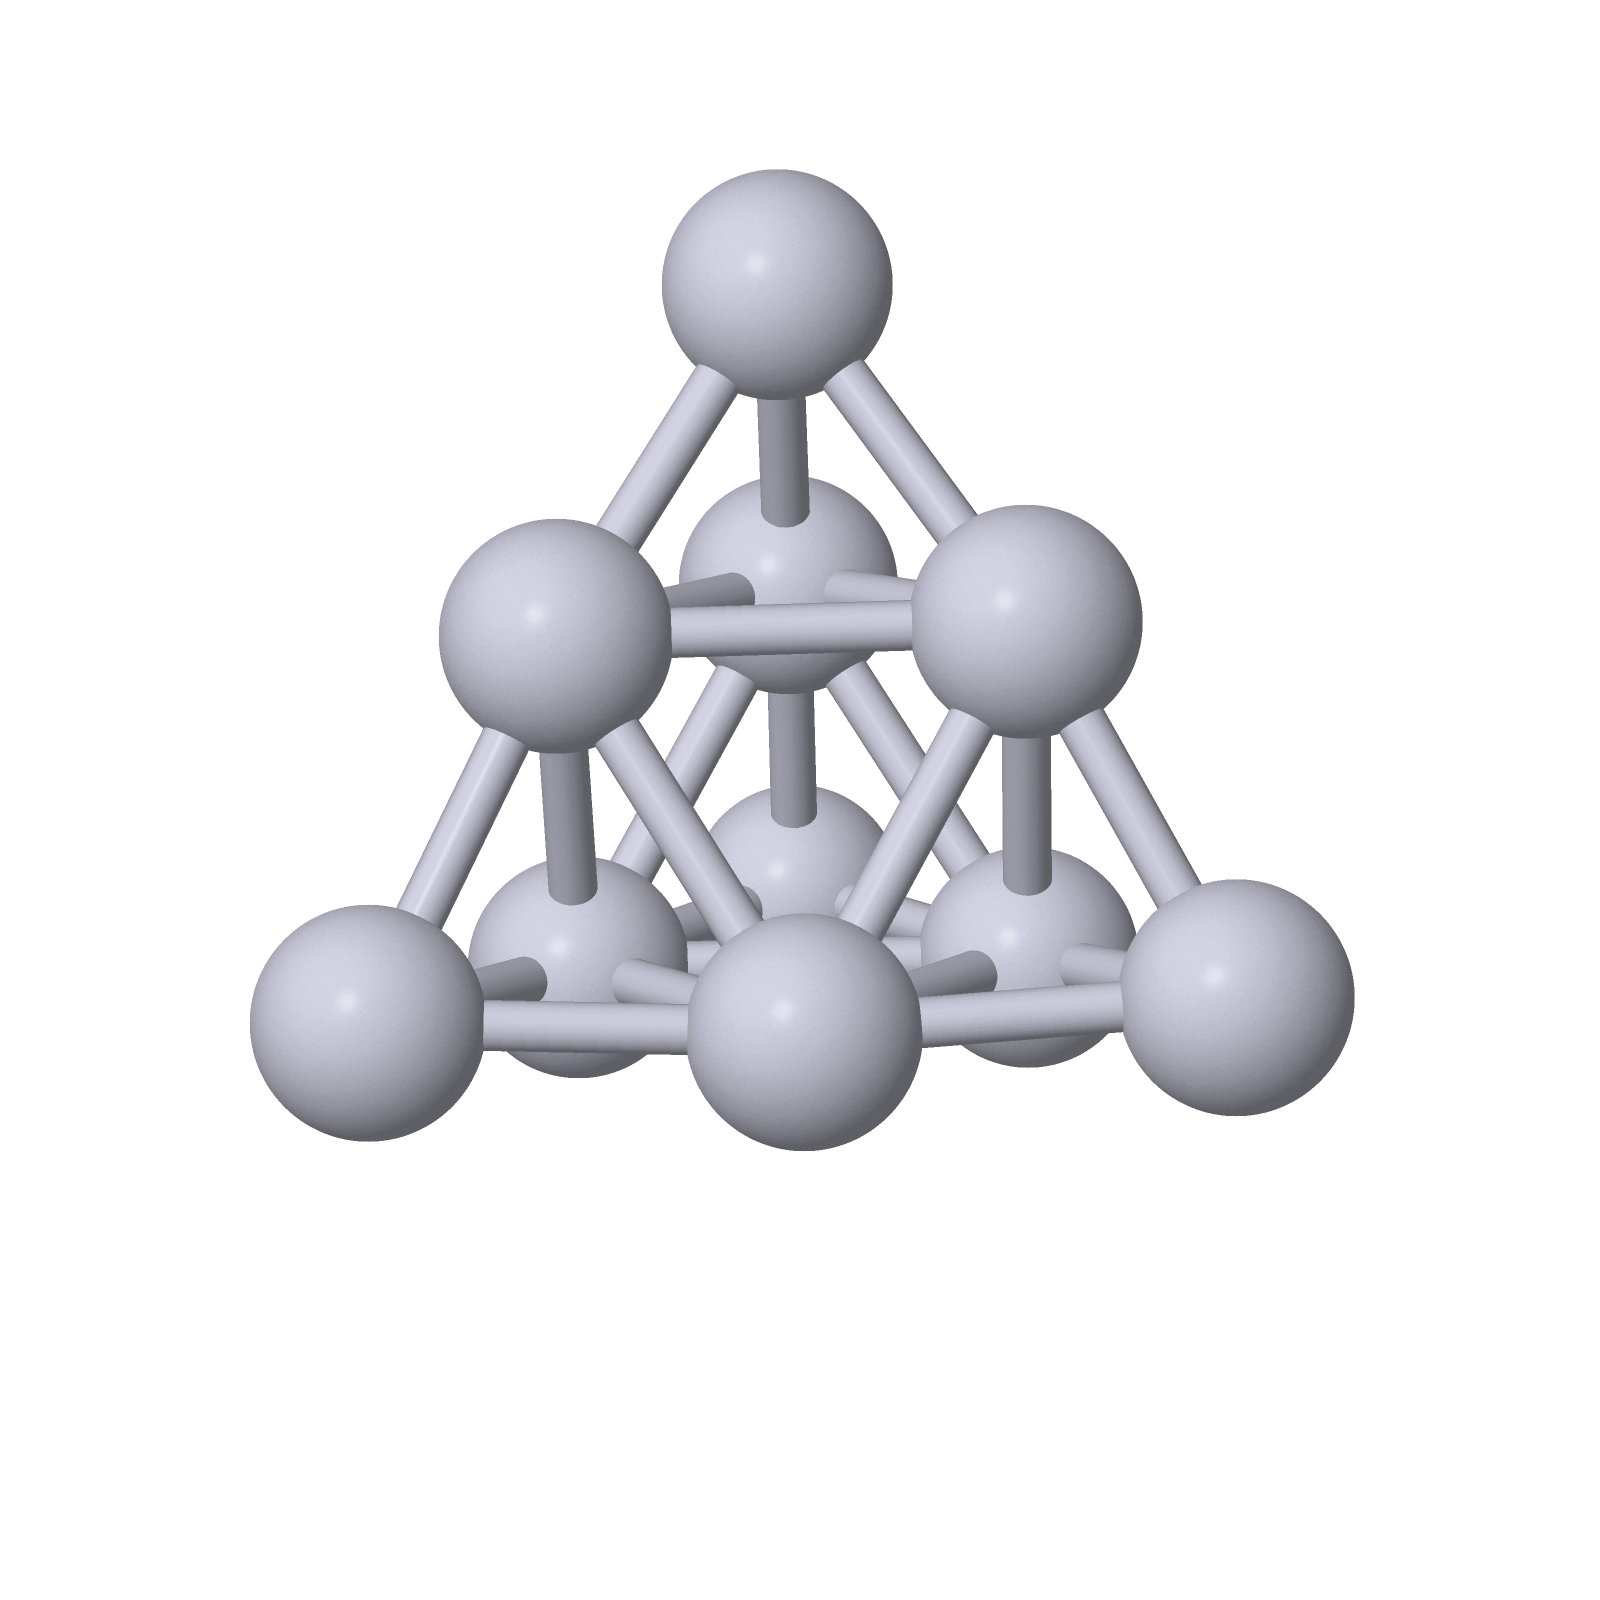
\includegraphics[width=\parentw]{pt10.png}};
\node[inner sep=0pt] (pt5ge5parent) at (3.45,2.75)
  {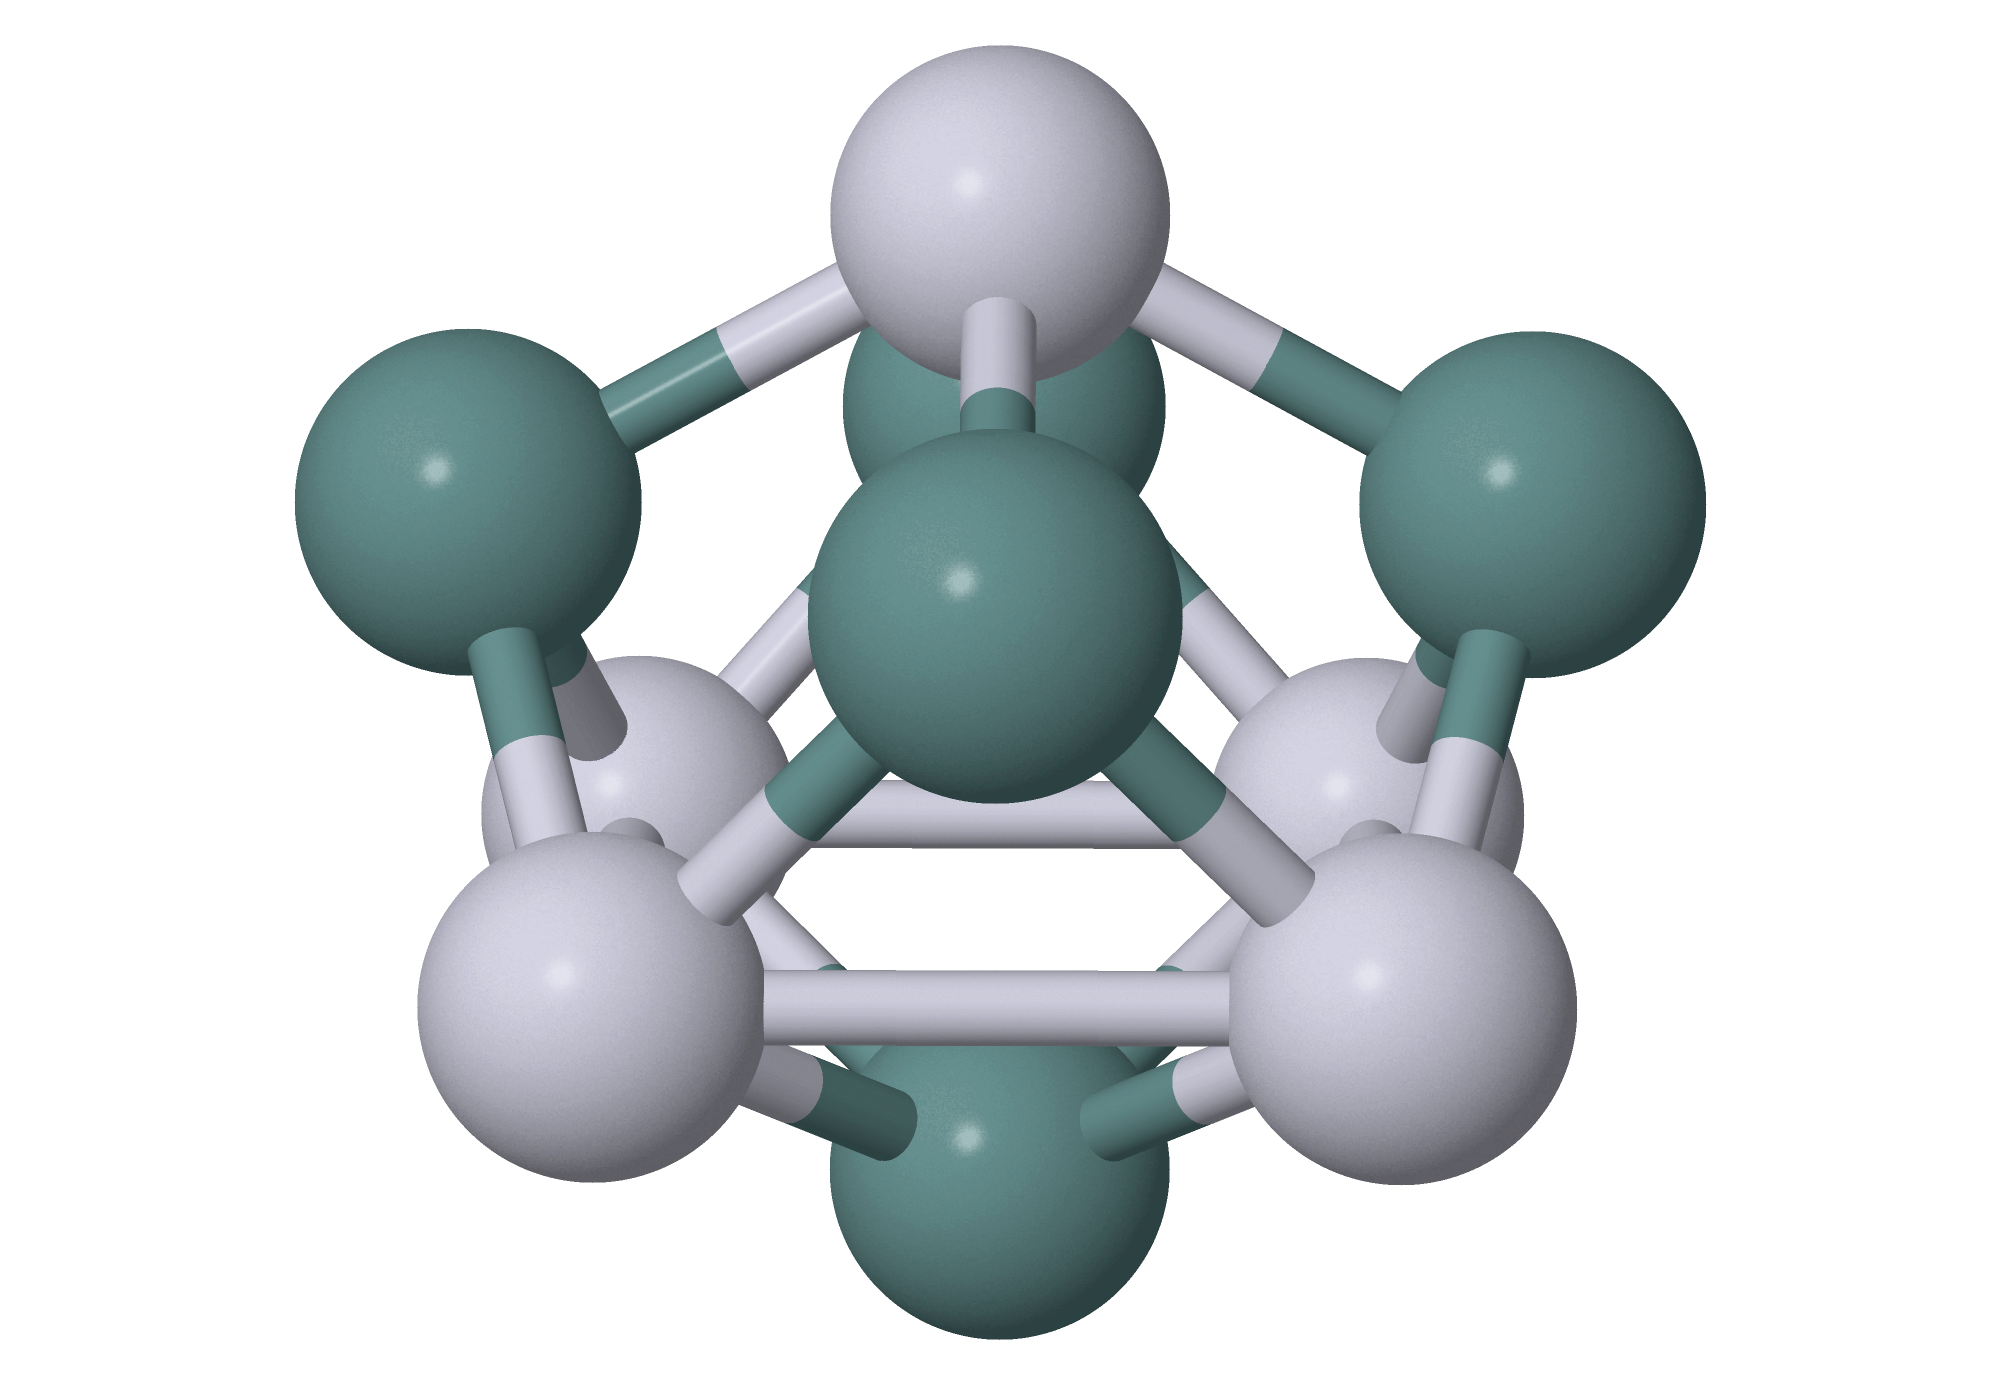
\includegraphics[width=\parentwide]{pt5ge5_orig.png}};

\node[inner sep=0pt] (pt6ge4) at (-5.15,-0.10)
  {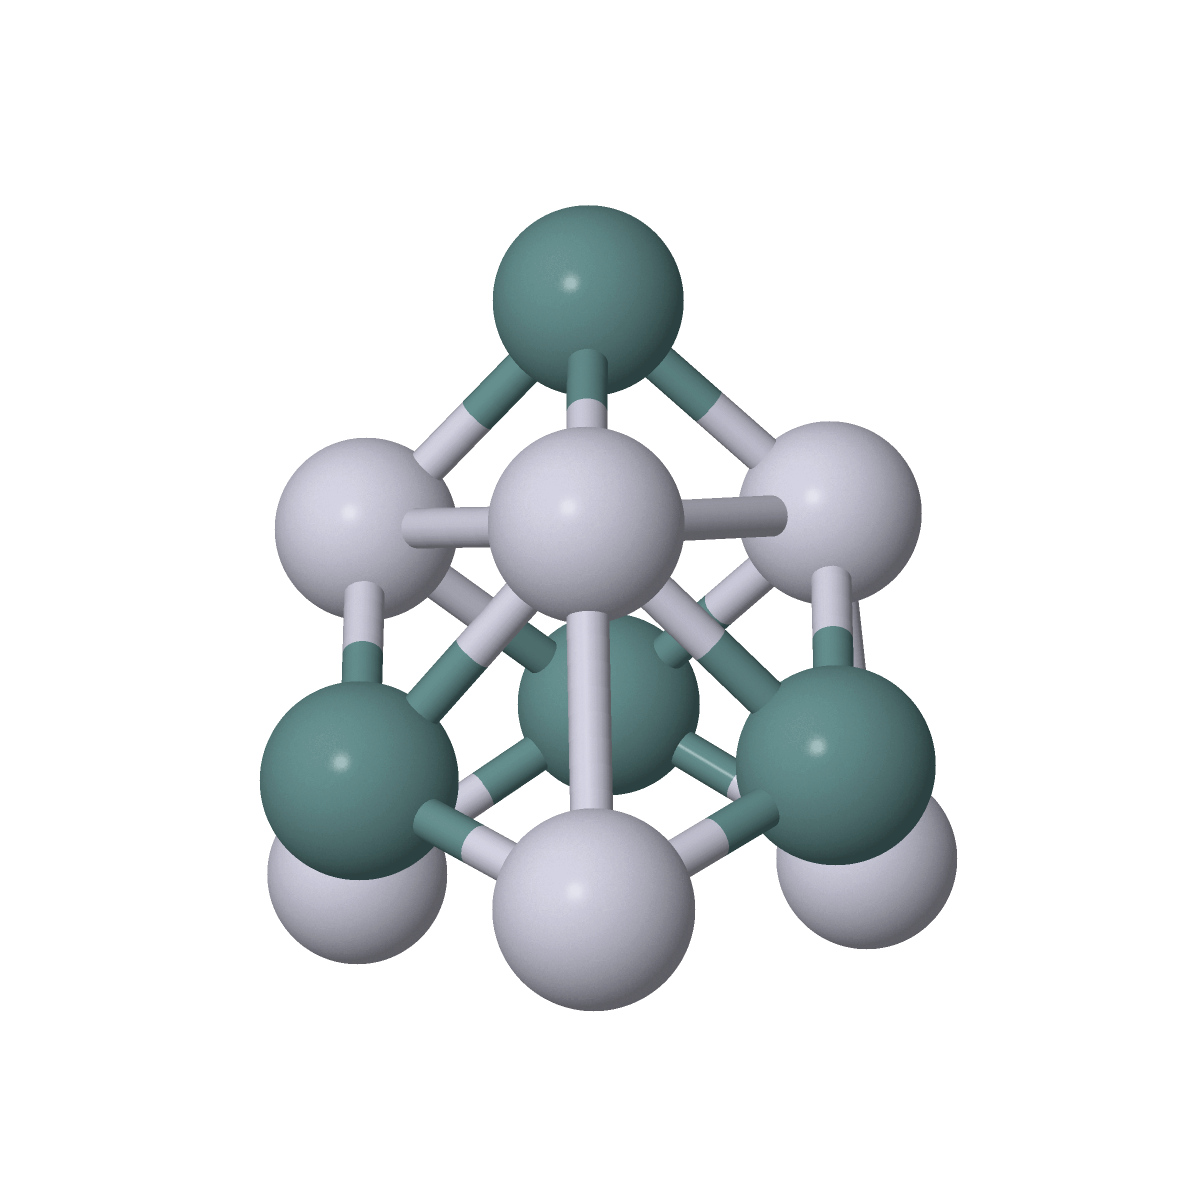
\includegraphics[width=\molw]{pt6ge4.png}};
\node[inner sep=0pt] (pt5ge5) at (-3.25,-0.10)
  {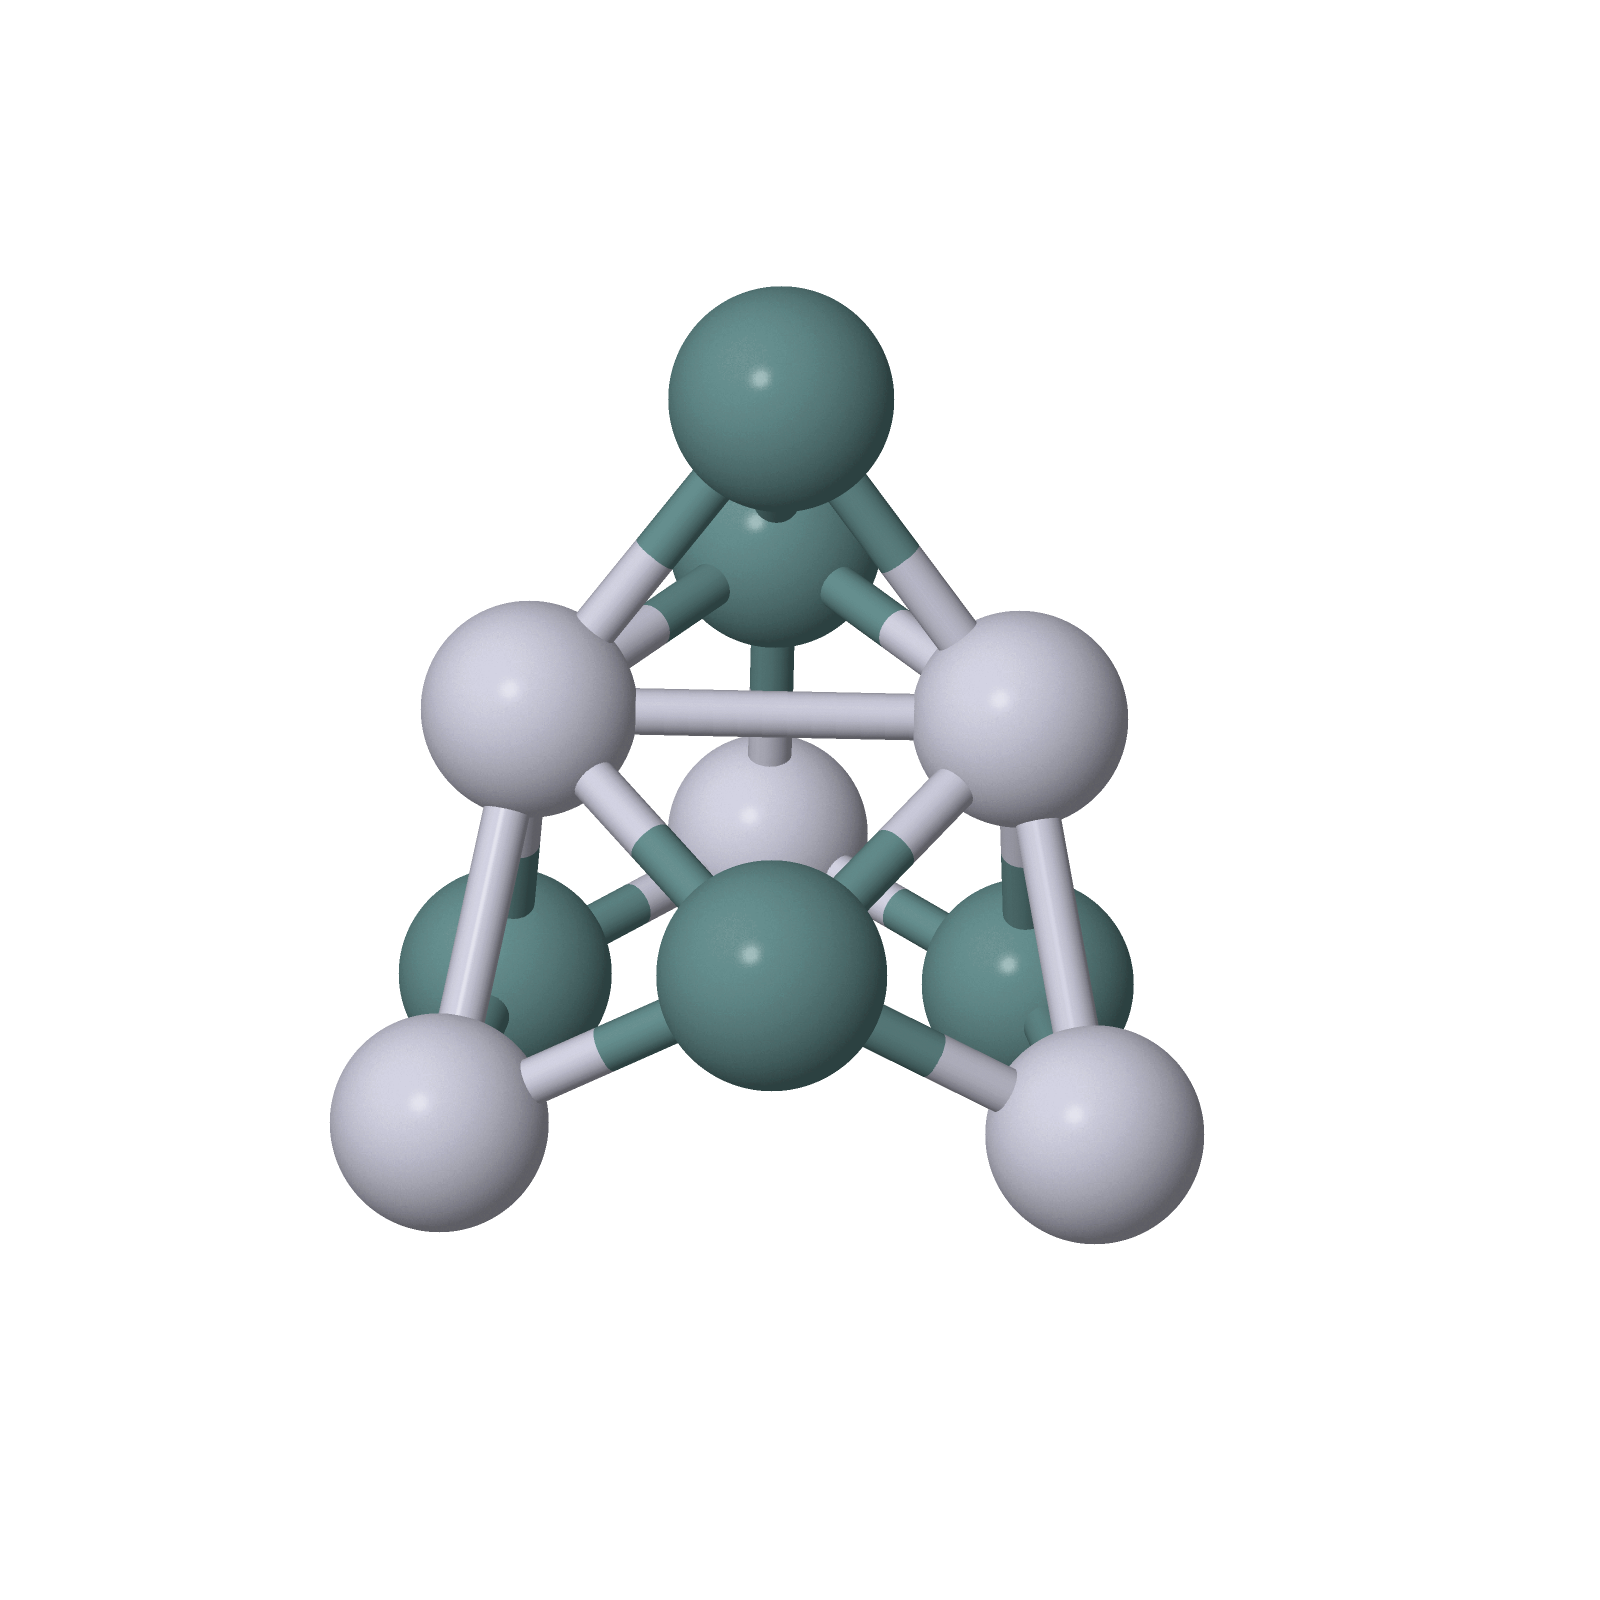
\includegraphics[width=\molw]{Pt5Ge5_fromPt10Parent.png}};
\node[inner sep=0pt] (pt4ge6) at (-1.15,-0.10)
  {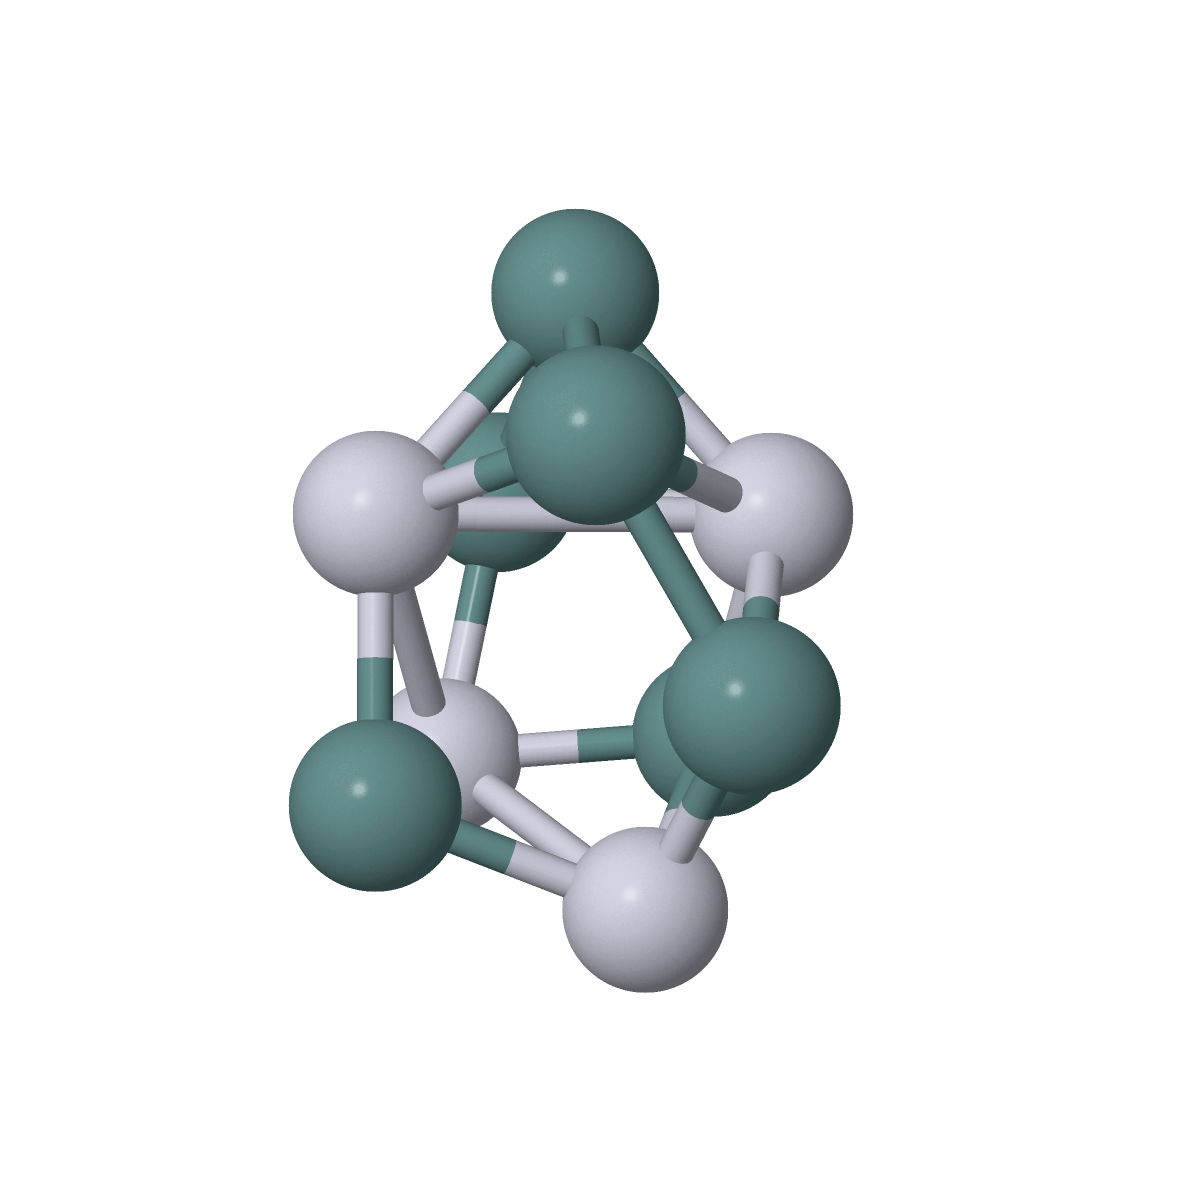
\includegraphics[width=\molw]{pt4ge6.png}};
\node[inner sep=0pt] (pt10frompt5ge5) at (3.45,-0.10)
  {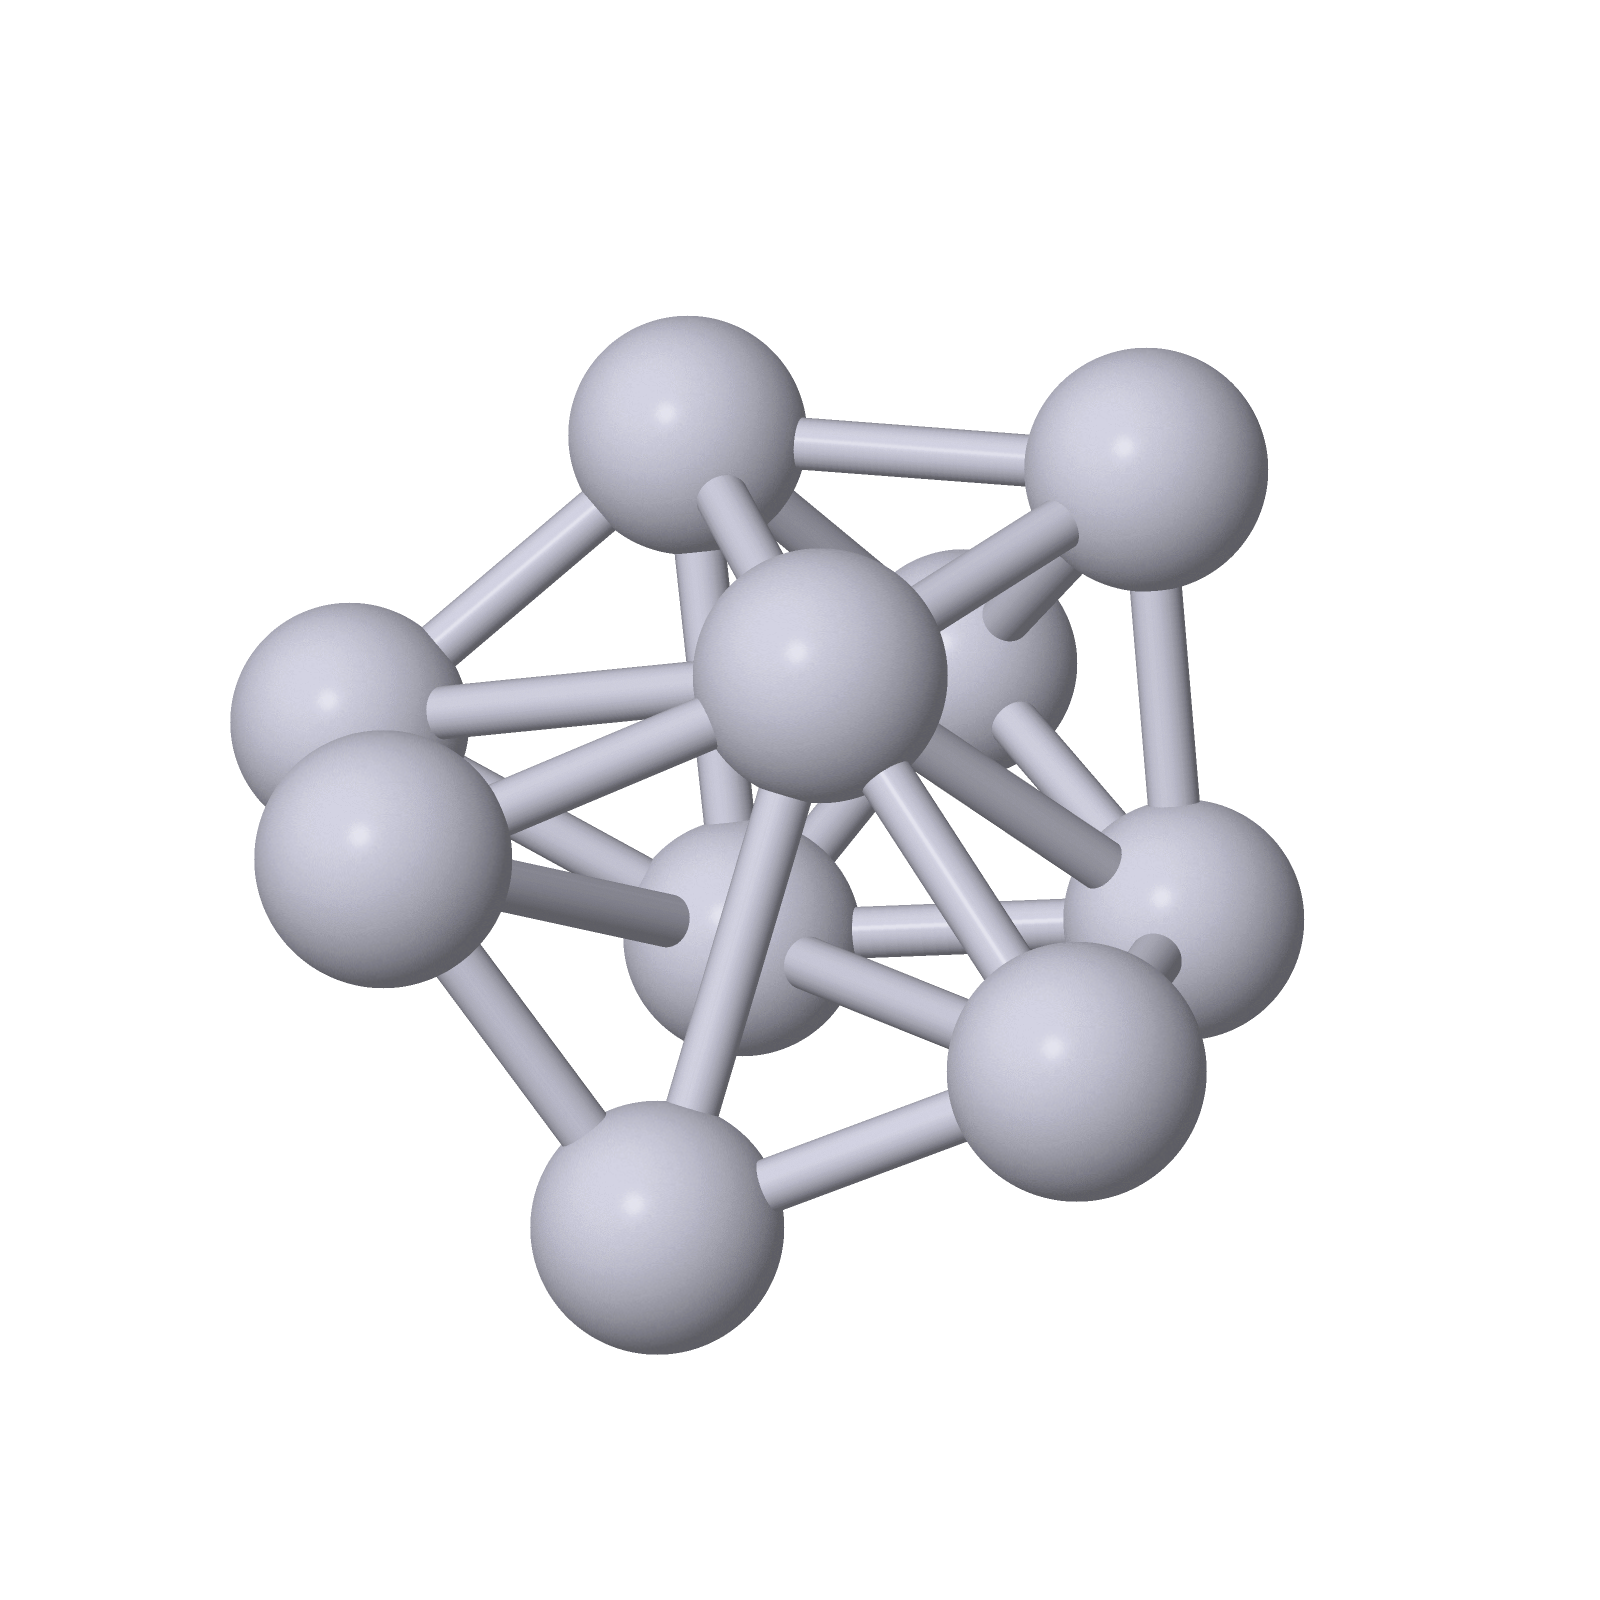
\includegraphics[width=\molwb]{pt10_from_pt5ge5.png}};

% Route arrows.
\draw[arrow] (-3.82,1.18) -- (-4.90,0.80);
\draw[arrow] (-3.30,1.18) -- (-3.25,0.82);
\draw[arrow] (-2.78,1.18) -- (-1.55,0.80);
\draw[arrow] (3.45,1.18) -- (3.45,0.85);

% Headers and labels.  Draw these last so they remain visible over the PNG
% image boxes.
\node[route] at (-3.30,4.58) {\ce{Pt10} parent framework};
\node[note] at (-3.30,4.16) {Ge substitution followed by optimization};
\node[route] at (3.45,4.58) {\ce{Pt5Ge5} parent framework};
\node[note] at (3.45,4.16) {Ge-to-Pt substitution followed by optimization};

\node[molname] at (-3.30,1.62) {\ce{Pt10} parent};
\node[molnote] at (-3.30,1.29) {reported framework};
\node[molname] at (3.45,1.62) {\ce{Pt5Ge5} parent};
\node[molnote] at (3.45,1.29) {reported framework};

\node[molname] at (-5.15,-1.18) {\ce{Pt6Ge4}};
\node[molnote] at (-5.15,-1.51) {from \ce{Pt10}};
\node[molname] at (-3.25,-1.18) {\ce{Pt5Ge5}};
\node[molnote] at (-3.25,-1.51) {from \ce{Pt10}};
\node[molname] at (-1.35,-1.18) {\ce{Pt4Ge6}};
\node[molnote] at (-1.35,-1.51) {from \ce{Pt10}};
\node[molname] at (3.45,-1.18) {\ce{Pt10}};
\node[molnote] at (3.45,-1.51) {from \ce{Pt5Ge5}};

\node[note] at (-0.70,-2.22)
  {Upper row: reported parent frameworks. Lower row: optimized crossed-parent derivatives.};

\end{tikzpicture}

\caption{Crossed-parent strategy used to examine the coupled effects of
composition and structural framework in the ten-atom clusters. Starting from
the reported global-minimum \ce{Pt10} framework, selected Pt atoms were
replaced by Ge and the resulting \ce{Pt6Ge4}, \ce{Pt5Ge5}, and \ce{Pt4Ge6}
structures were optimized. In the reverse construction, the reported
global-minimum \ce{Pt5Ge5} framework was converted into a pure \ce{Pt10}
derivative and then optimized. The snapshots
shown in the upper row correspond to the reported parent frameworks, whereas
the lower row shows the optimized crossed-parent derivatives used in the
present study.}
\label{fig:crossed_models}
\end{figure}

At the PBEPBE/def2-TZVP level, the \ce{Pt10} structure derived from the
\ce{Pt5Ge5} framework is lowest as a triplet, and the quintet is 0.0413 eV
higher in $\Delta E_0$. The selected triplet wavefunction and the seven
distinct triplet \ce{Pt10CO} minima were confirmed to be orbital-stable. The three
Ge-containing derivatives generated from the \ce{Pt10} parent framework favor
the closed-shell singlet over the triplet by 0.176--0.263 eV. Thus, within this
set of models, the Ge-containing clusters have a clearer preference for
the low-spin state than the pure-\ce{Pt10} derivative.

\subsubsection{Bonding patterns in the crossed-parent clusters}

AdNDP was used to compare localized two-center bonding with delocalized
multicenter bonding in the crossed-parent structures.\cite{zubarev:adndp:2008,
tkachenko:adndp2:2019}
For the triplet \ce{Pt10}, the $alpha$ and $beta$ density
matrices were analyzed separately. Each channel gives 30 Pt-centered 1c
elements, with three on every Pt atom. Nineteen 3c elements occur on the same
atomic centers in both channels. Their combined alpha+beta occupation numbers
are 1.984--1.994, so they are assigned as 19 3c--2e elements. The alpha
channel contains two additional 3c elements, % on Pt(2)--Pt(3)--Pt(7) and Pt(5)--Pt(6)--Pt(10), 
each with an occupation number of about 0.994. These are
assigned as two 3c--1e elements and account for the two excess alpha electrons
of the triplet. The large number of high-occupation 3c elements distributed
over the Pt framework supports a delocalized multicenter bonding description.
The complete spin-resolved decomposition and occupation ranges are reported
in Supporting Table~\ref{tab:tfg_adndp_summary}.

This spin-resolved pattern agrees qualitatively with the earlier AdNDP analysis of the
lowest-energy high-spin \ce{Pt10} cluster. That structure was described by 30
one-center pairs, 16 3c--2e bonds, four 3c--1e bonds, and four 4c--1e
bonds.\cite{ugartemendia:2022} The exact numbers are different because the two
\ce{Pt10} structures and spin states are different, but both analyses describe
bonding in pure Pt clusters as mainly delocalized and multicenter.
In contrast, the Ge-containing clusters favor more localized elements. The \ce{Pt5Ge5}
derivative obtained from the \ce{Pt10} framework is dominated by localized
Pt--Ge and Pt--Pt two-center bonds, although one four-center element remains.
The \ce{Pt6Ge4} and \ce{Pt4Ge6} models also favor mainly one- and two-center
elements. The starting geometry affects the detailed bonding pattern, while
Ge substitution favors a more localized and covalent bonding framework.
Representative multicenter and two-center AdNDP elements are shown in
Figure~\ref{fig:tfg_adndp_comparison}. The numerical summaries, occupation
ranges, and search thresholds are given in Supporting Table~\ref{tab:tfg_adndp_summary}.

\begin{figure}[H]
\centering
\begin{tikzpicture}[
  x=1cm,
  y=1cm,
  panel/.style={font=\sffamily\bfseries\small, anchor=north west, fill=white,
    fill opacity=0.86, text opacity=1, inner sep=2pt},
  %label/.style={font=\sffamily\bfseries\small, align=center},
  label/.style={font=\sffamily\small, align=center},
  note/.style={font=\sffamily\scriptsize, align=center, text=black!70,
    text width=0.28\linewidth}
]

% Panel sizes and positions can be tuned directly from here.
\def\adndpw{0.305\linewidth}
\def\yimage{0}
\def\ylabel{-2.42}
\def\ynote{-3.15}

\node[inner sep=0pt] (pt10c) at (-4.35,\yimage)
  {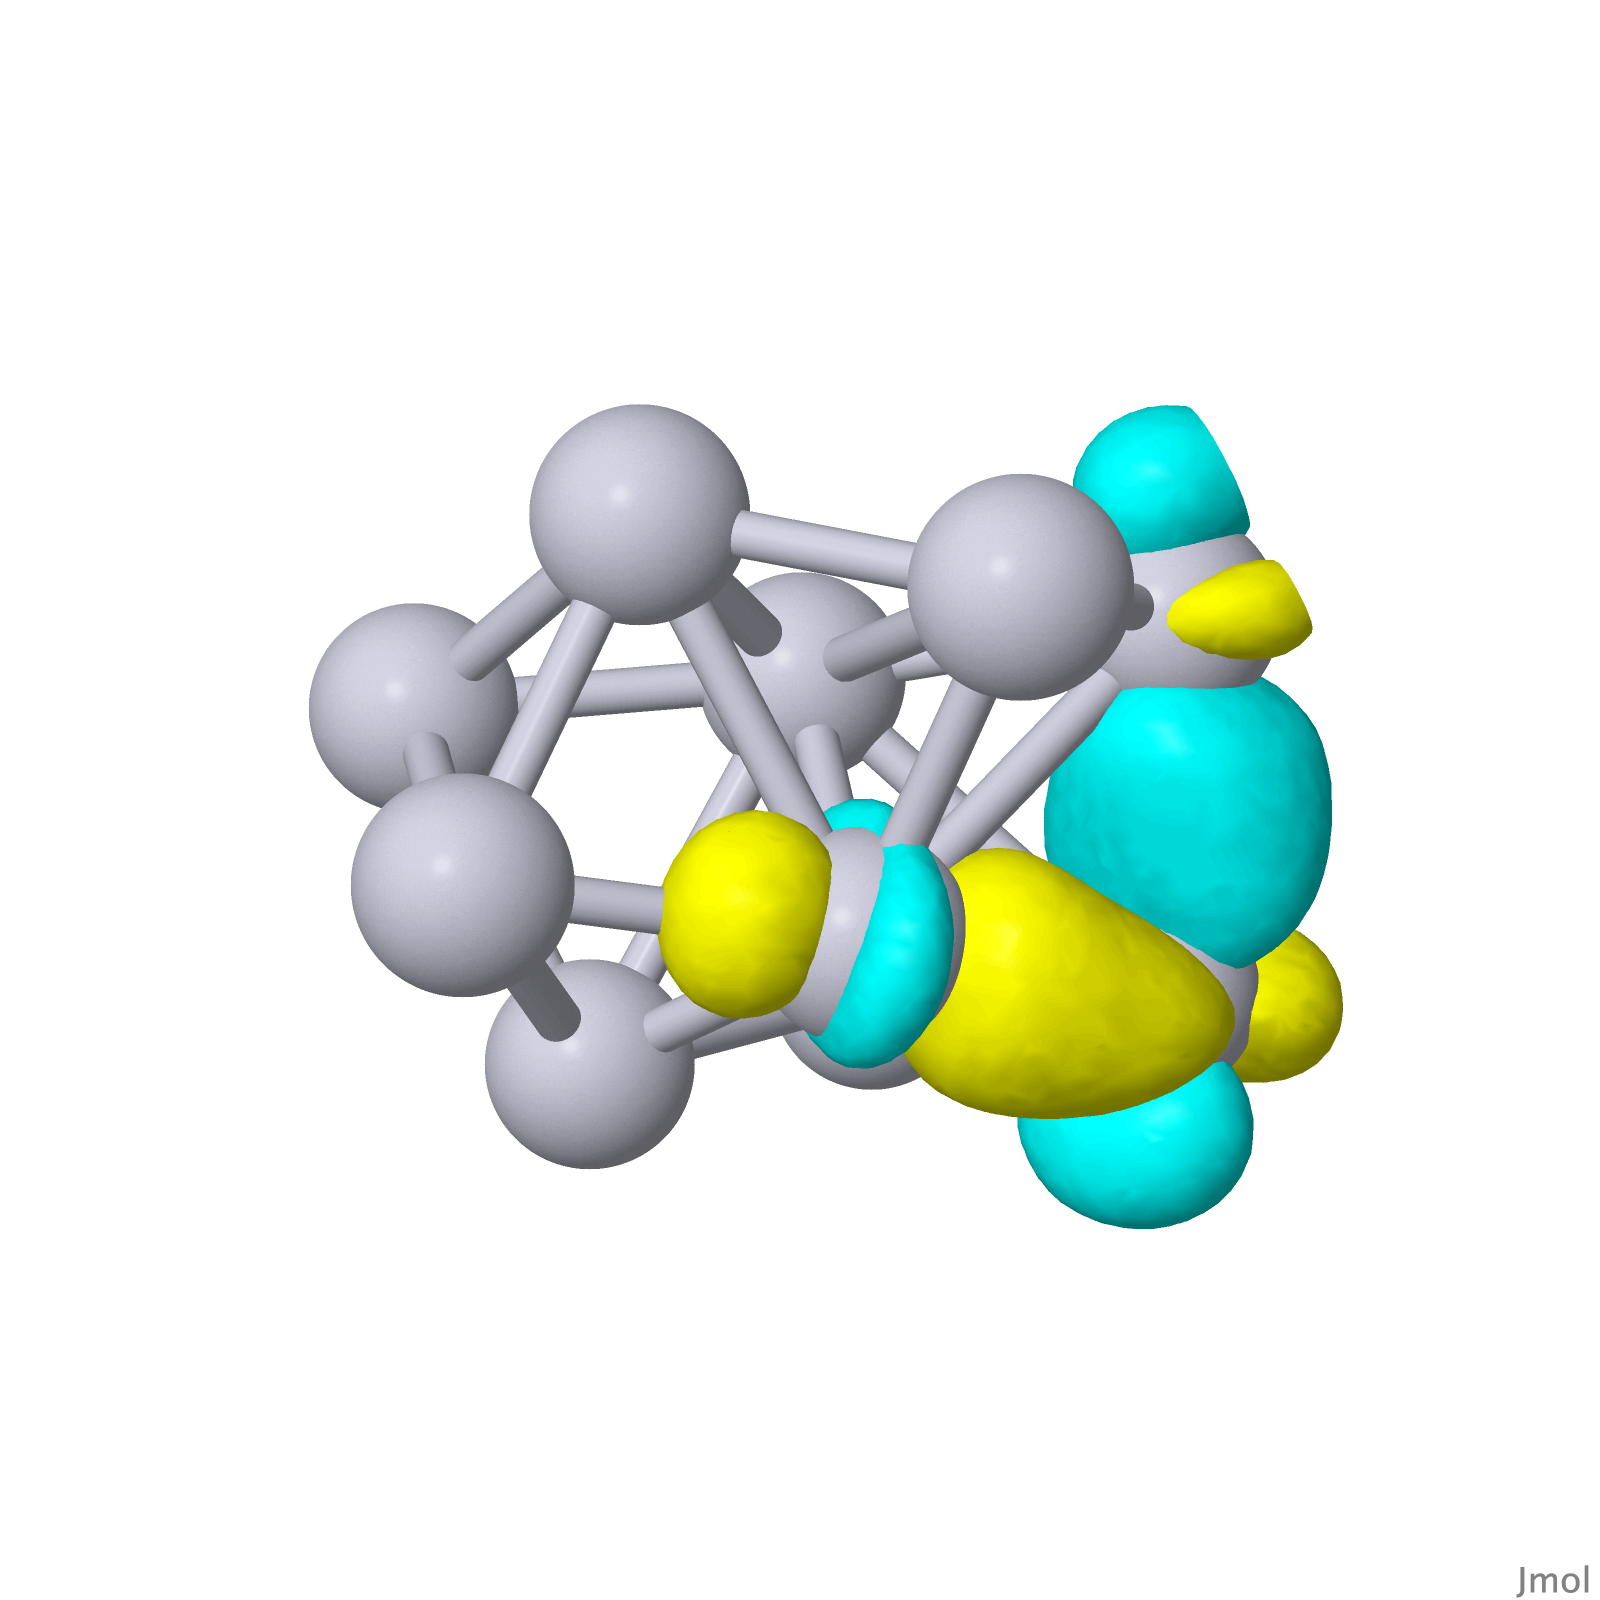
\includegraphics[width=\adndpw]{adndp_pt10_3c.png}};
\node[inner sep=0pt] (pt5ge2c) at (0,\yimage)
  {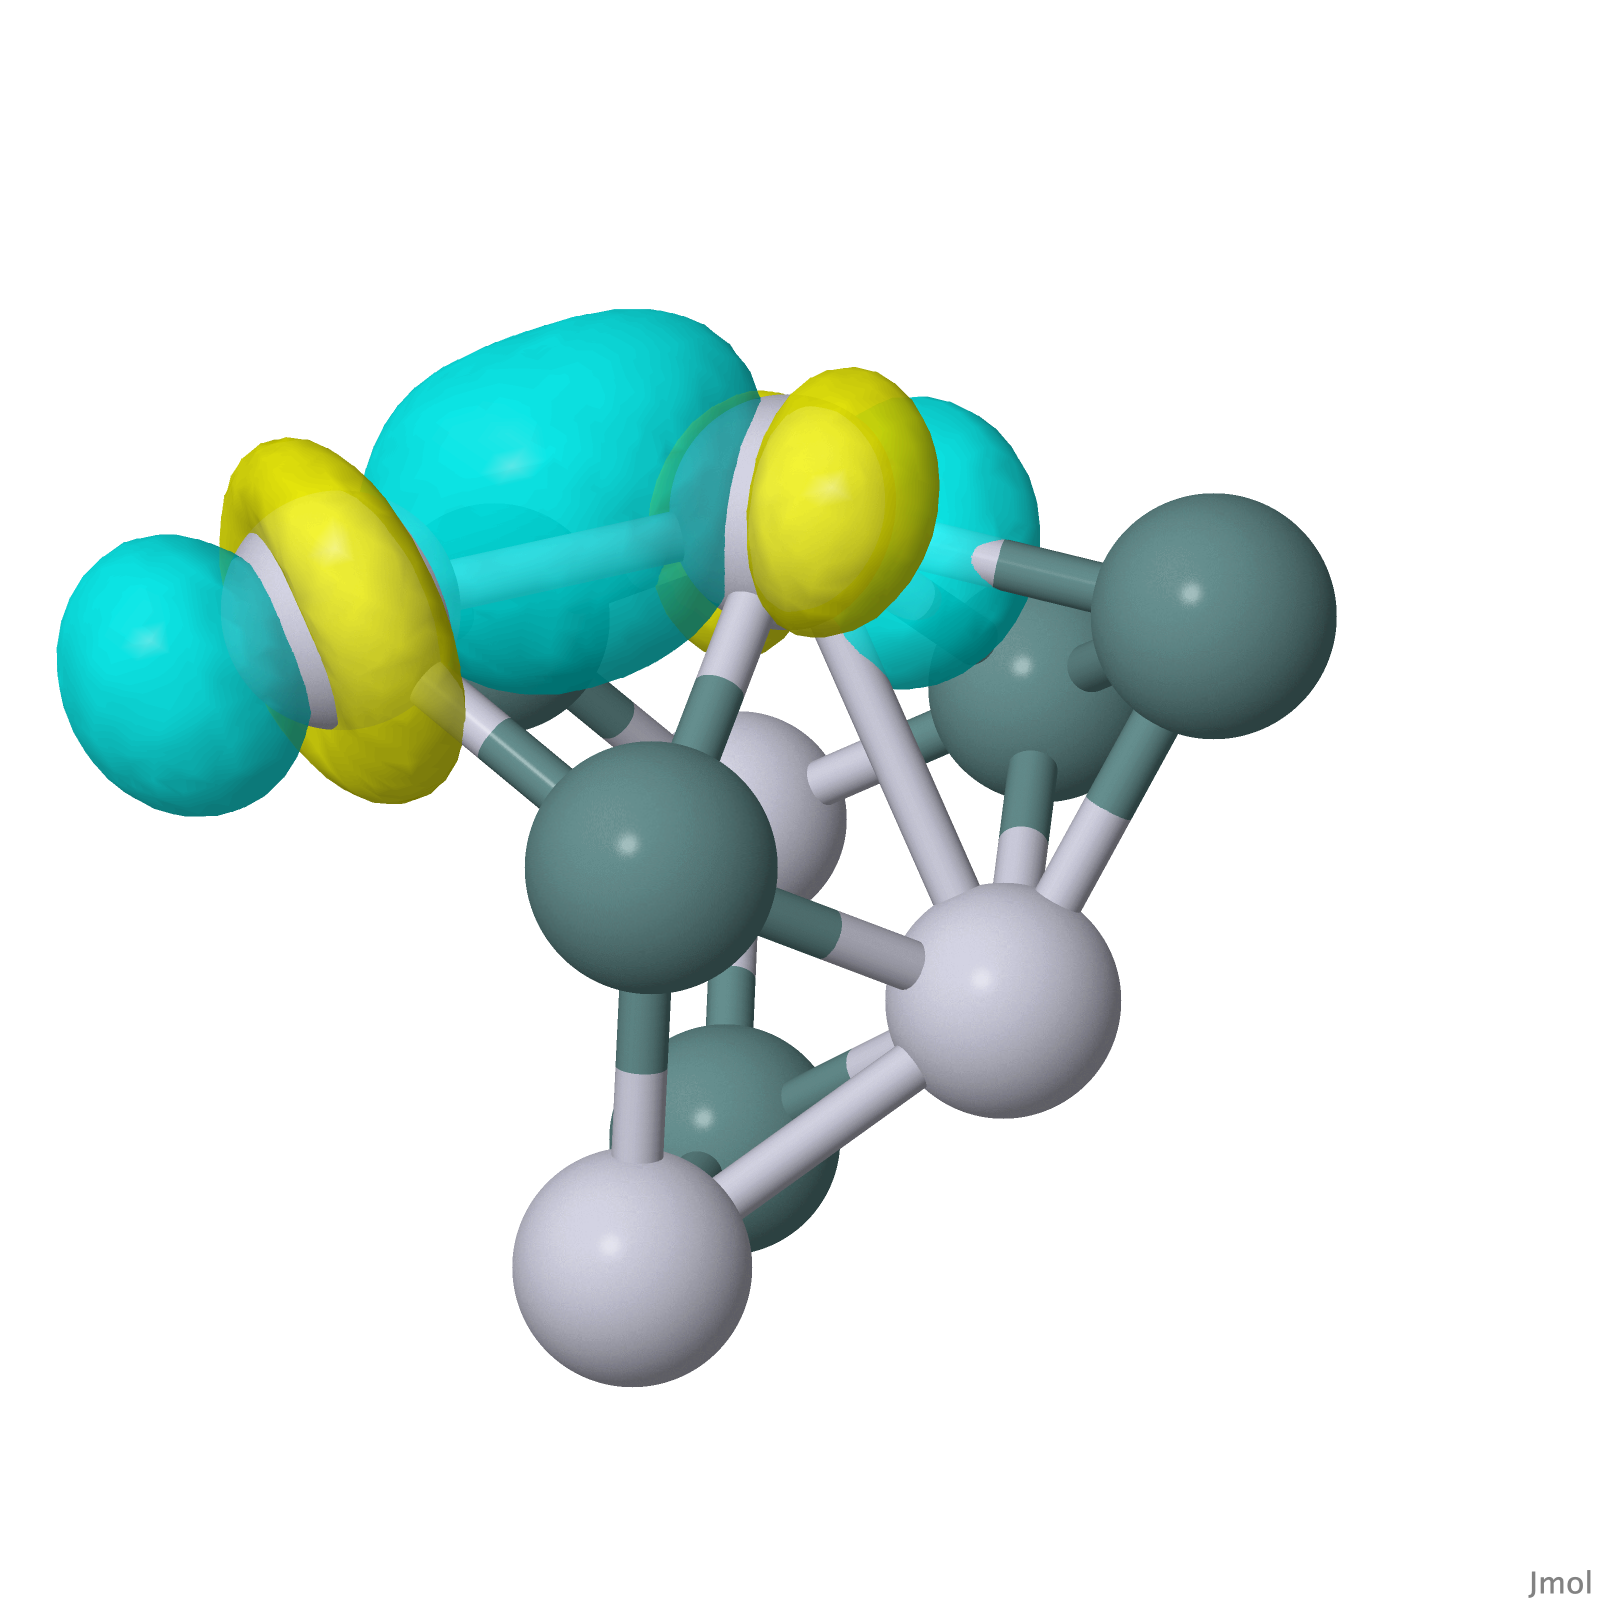
\includegraphics[width=\adndpw]{adndp_pt5ge_2c2e.png}};
\node[inner sep=0pt] (pt5ge4c) at (4.15,\yimage)
  {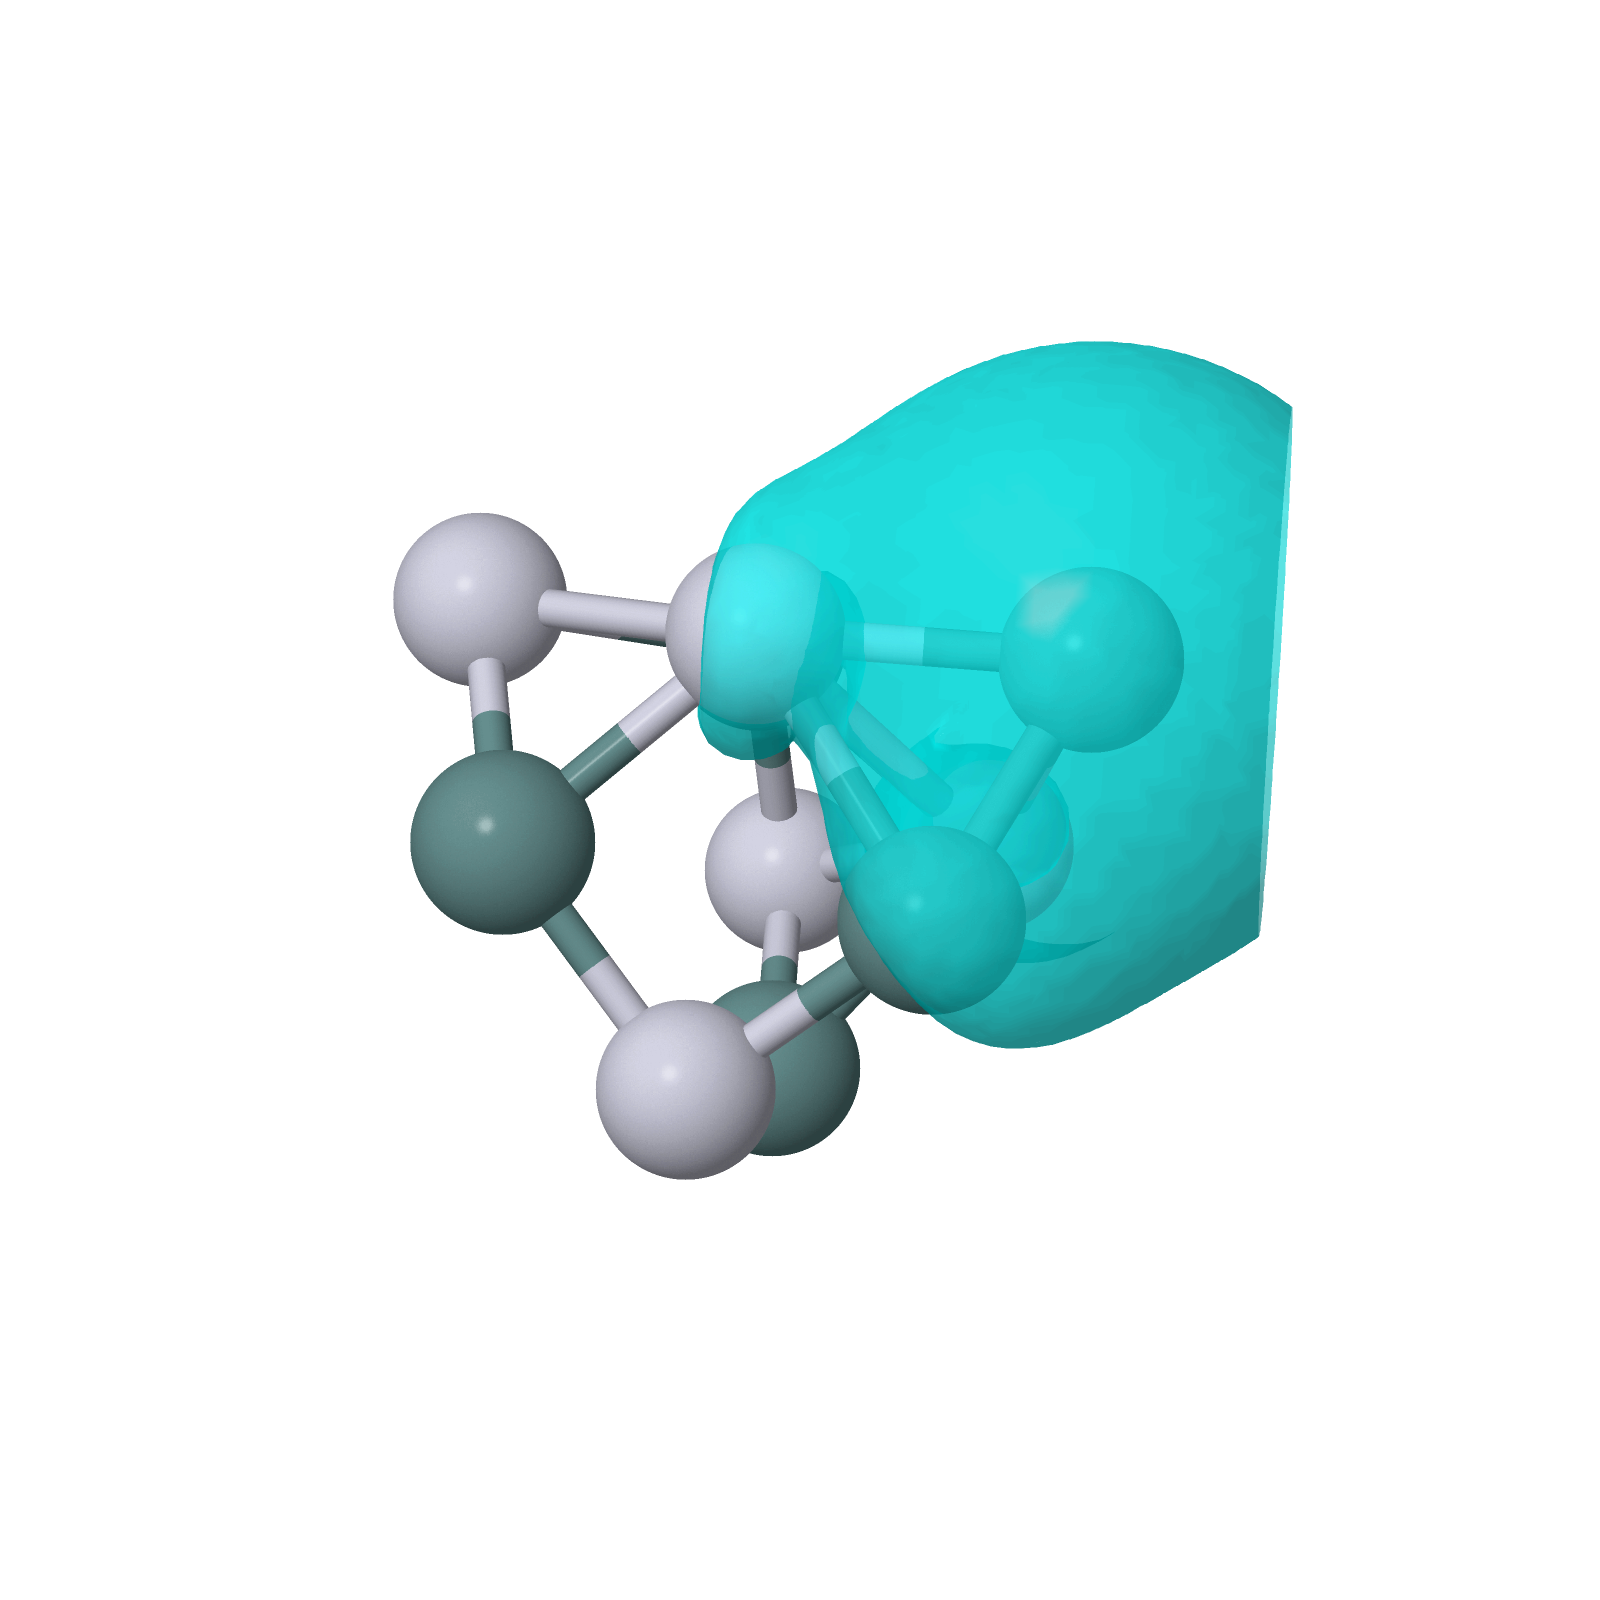
\includegraphics[width=\adndpw]{adndp_pt5ge_4c2e.png}};

\node[panel] at ([xshift=-1.72cm,yshift=1.82cm]pt10c.center) {(a)};
\node[panel] at ([xshift=-1.72cm,yshift=1.82cm]pt5ge2c.center) {(b)};
\node[panel] at ([xshift=-1.72cm,yshift=1.82cm]pt5ge4c.center) {(c)};

\node[label] at (-4.15,\ylabel) {\ce{Pt10}};
\node[note] at (-4.15,\ynote) {representative\\3c topology};
\node[label] at (0,\ylabel) {\ce{Pt5Ge5}};
\node[note] at (0,\ynote) {representative Pt--Ge\\2c--2e element};
\node[label] at (4.15,\ylabel) {\ce{Pt5Ge5}};
\node[note] at (4.15,\ynote) {residual\\4c--2e element};

\end{tikzpicture}

\caption{Representative AdNDP elements showing the change from multicenter
metallic bonding in the pure \ce{Pt10} derivative to predominantly localized
two-center bonding in the Ge-containing models: (a) a 3c element of triplet
\ce{Pt10}, (b) a Pt--Ge 2c--2e element of \ce{Pt5Ge5}, and (c) the residual
4c--2e element of \ce{Pt5Ge5}. Panel (a) shows the spatial form of one of the
3c elements identified in the spin-resolved analysis.}
\label{fig:tfg_adndp_comparison}
\end{figure}



\subsubsection[CO adsorption energies]{\ce{CO} adsorption energies}

We next compare \ce{CO} adsorption across the different compositions and parent
structures. Selected spin states are included to check whether they change the
main adsorption patterns. The primary data set is the crossed-parent series described
above. We compare it with a second set obtained by placing \ce{CO} at the
independent Pt sites of the previously reported global-minimum structures of
the same compositions.\cite{ugartemendia:2022} This comparison shows how the
calculated adsorption changes when a different parent geometry or spin state
is used. Figure~\ref{fig:neutral_data_sets} summarizes the relation between
the two sets.


The labels shown in Figure~\ref{fig:tfg_site_numbering} identify the initial
adsorption positions. Because these clusters are flexible, different starting
positions can converge to the same optimized carbonyl minimum after the
cluster and the adsorbate relax.

\begin{figure}[H]
\centering
\begin{tikzpicture}[
  x=1cm,
  y=1cm,
  panel/.style={font=\sffamily\small, anchor=north west, fill=white,
    fill opacity=0.90, text opacity=1, inner sep=2pt},
  title/.style={font=\sffamily\small, align=center},
  note/.style={font=\sffamily\scriptsize, align=center, text=black!70},
  sitelabel/.style={draw=black,
	  circle, fill=white, line width=0.5pt,
	  draw=none,
	  draw opacity=1,
	  fill opacity=0.05,
      text opacity=0.5,
      minimum size=4.8mm, inner sep=0pt, font=\sffamily\bfseries\scriptsize
}
]

% Layout controls.
\def\imgw{0.265\linewidth}
\def\leftx{-3.45}
\def\rightx{3.45}
\def\topy{2.45}
\def\bottomy{-2.75}
\def\titleshift{-2.05cm}

% Bare crossed-parent models.
\node[inner sep=0pt] (pt10cross) at (\leftx,\topy)
  {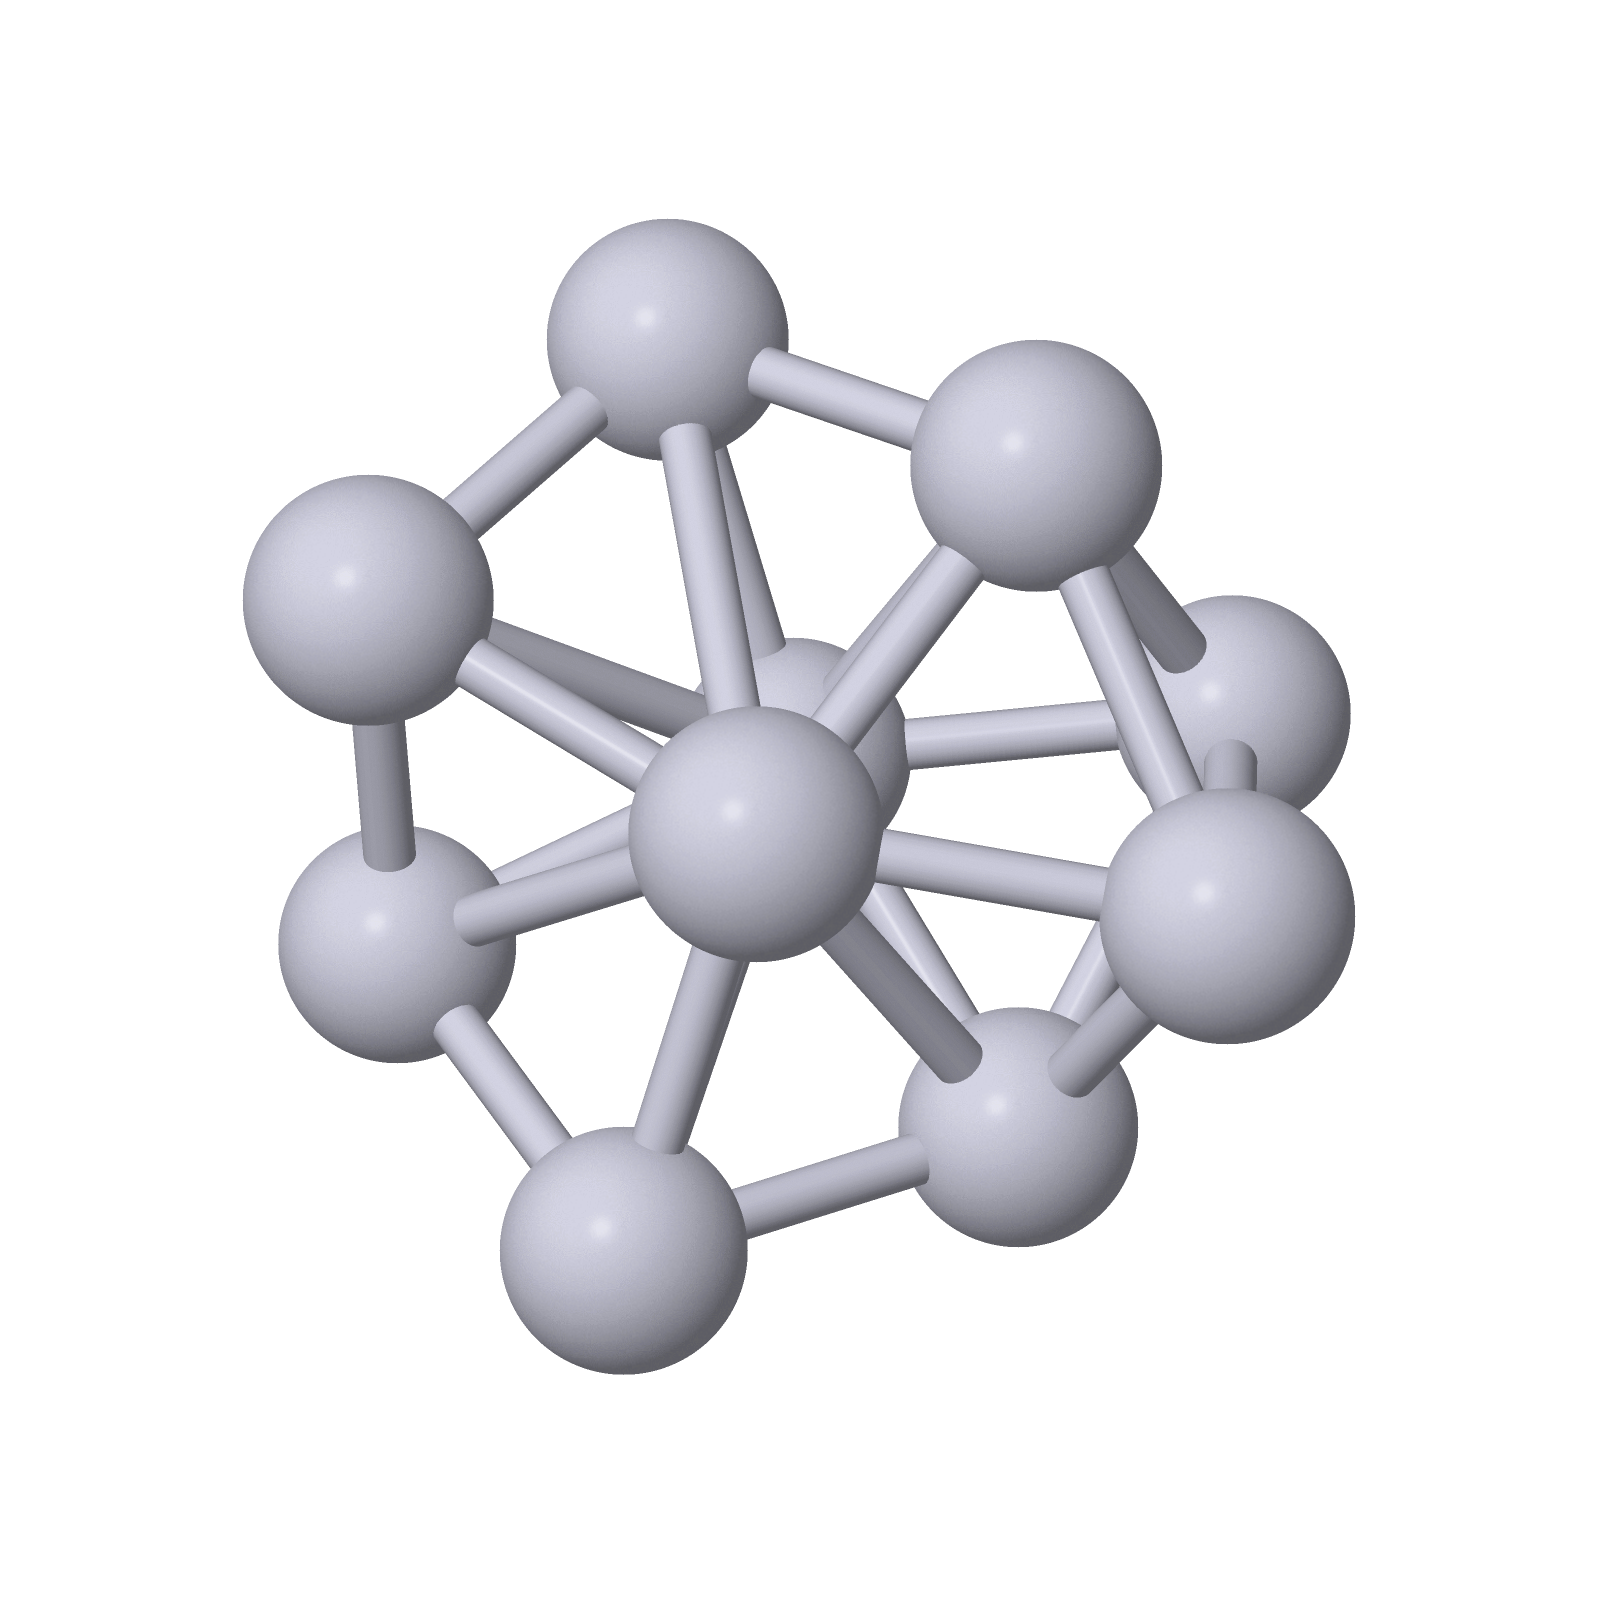
\includegraphics[width=\imgw]{Pt10CO/pt10_ref.png}};
\node[inner sep=0pt] (pt6ge4cross) at (\rightx,\topy)
  {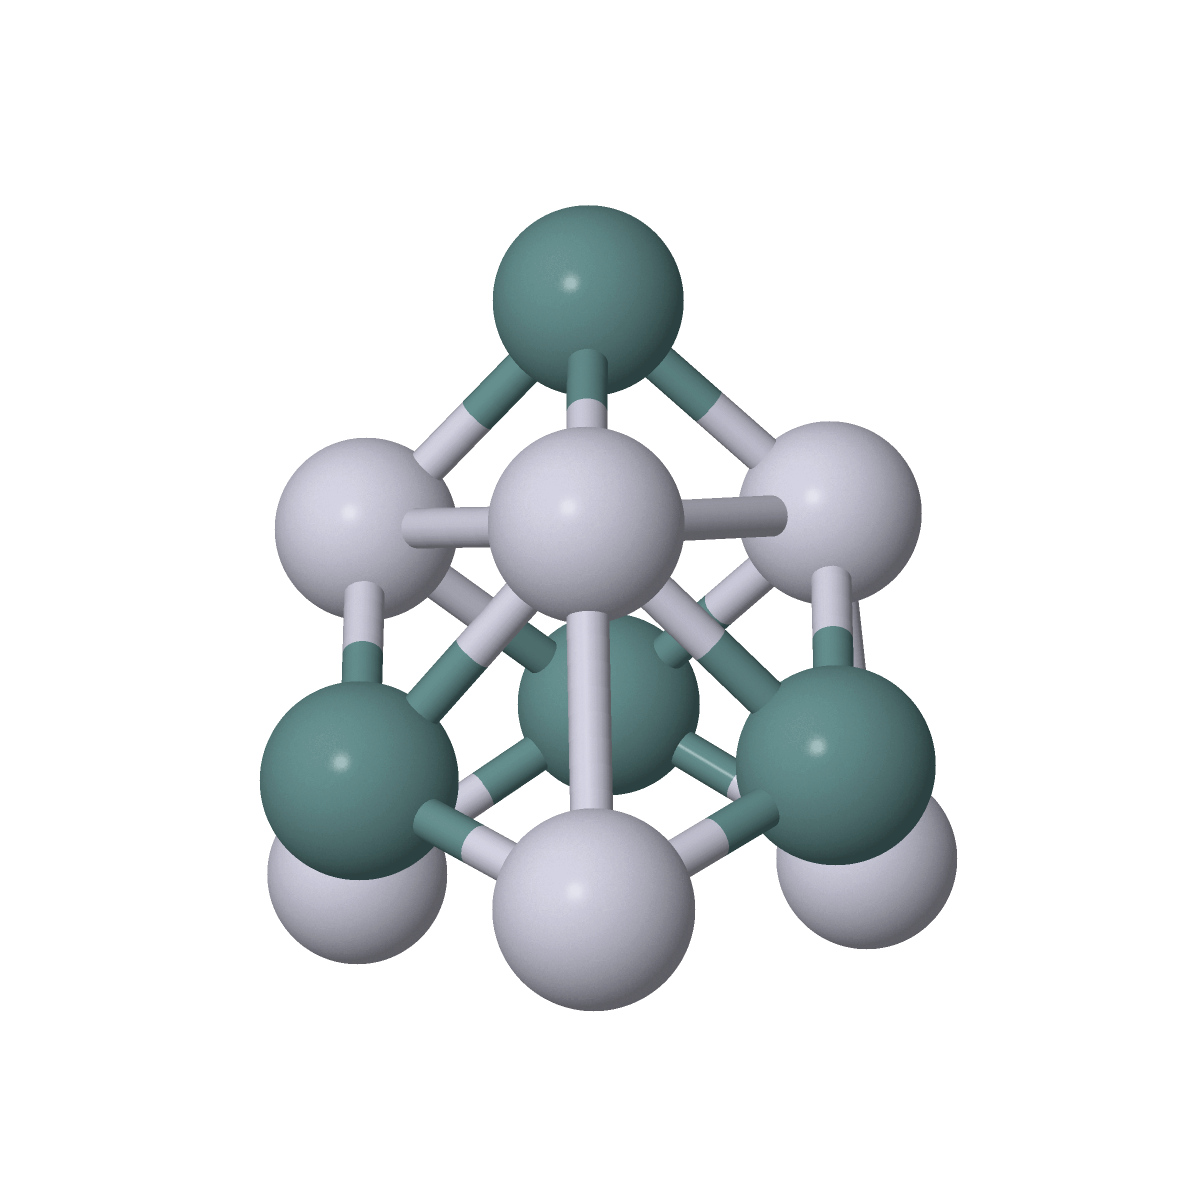
\includegraphics[width=\imgw]{pt6ge4.png}};
\node[inner sep=0pt] (pt5ge5cross) at (\leftx,\bottomy)
  {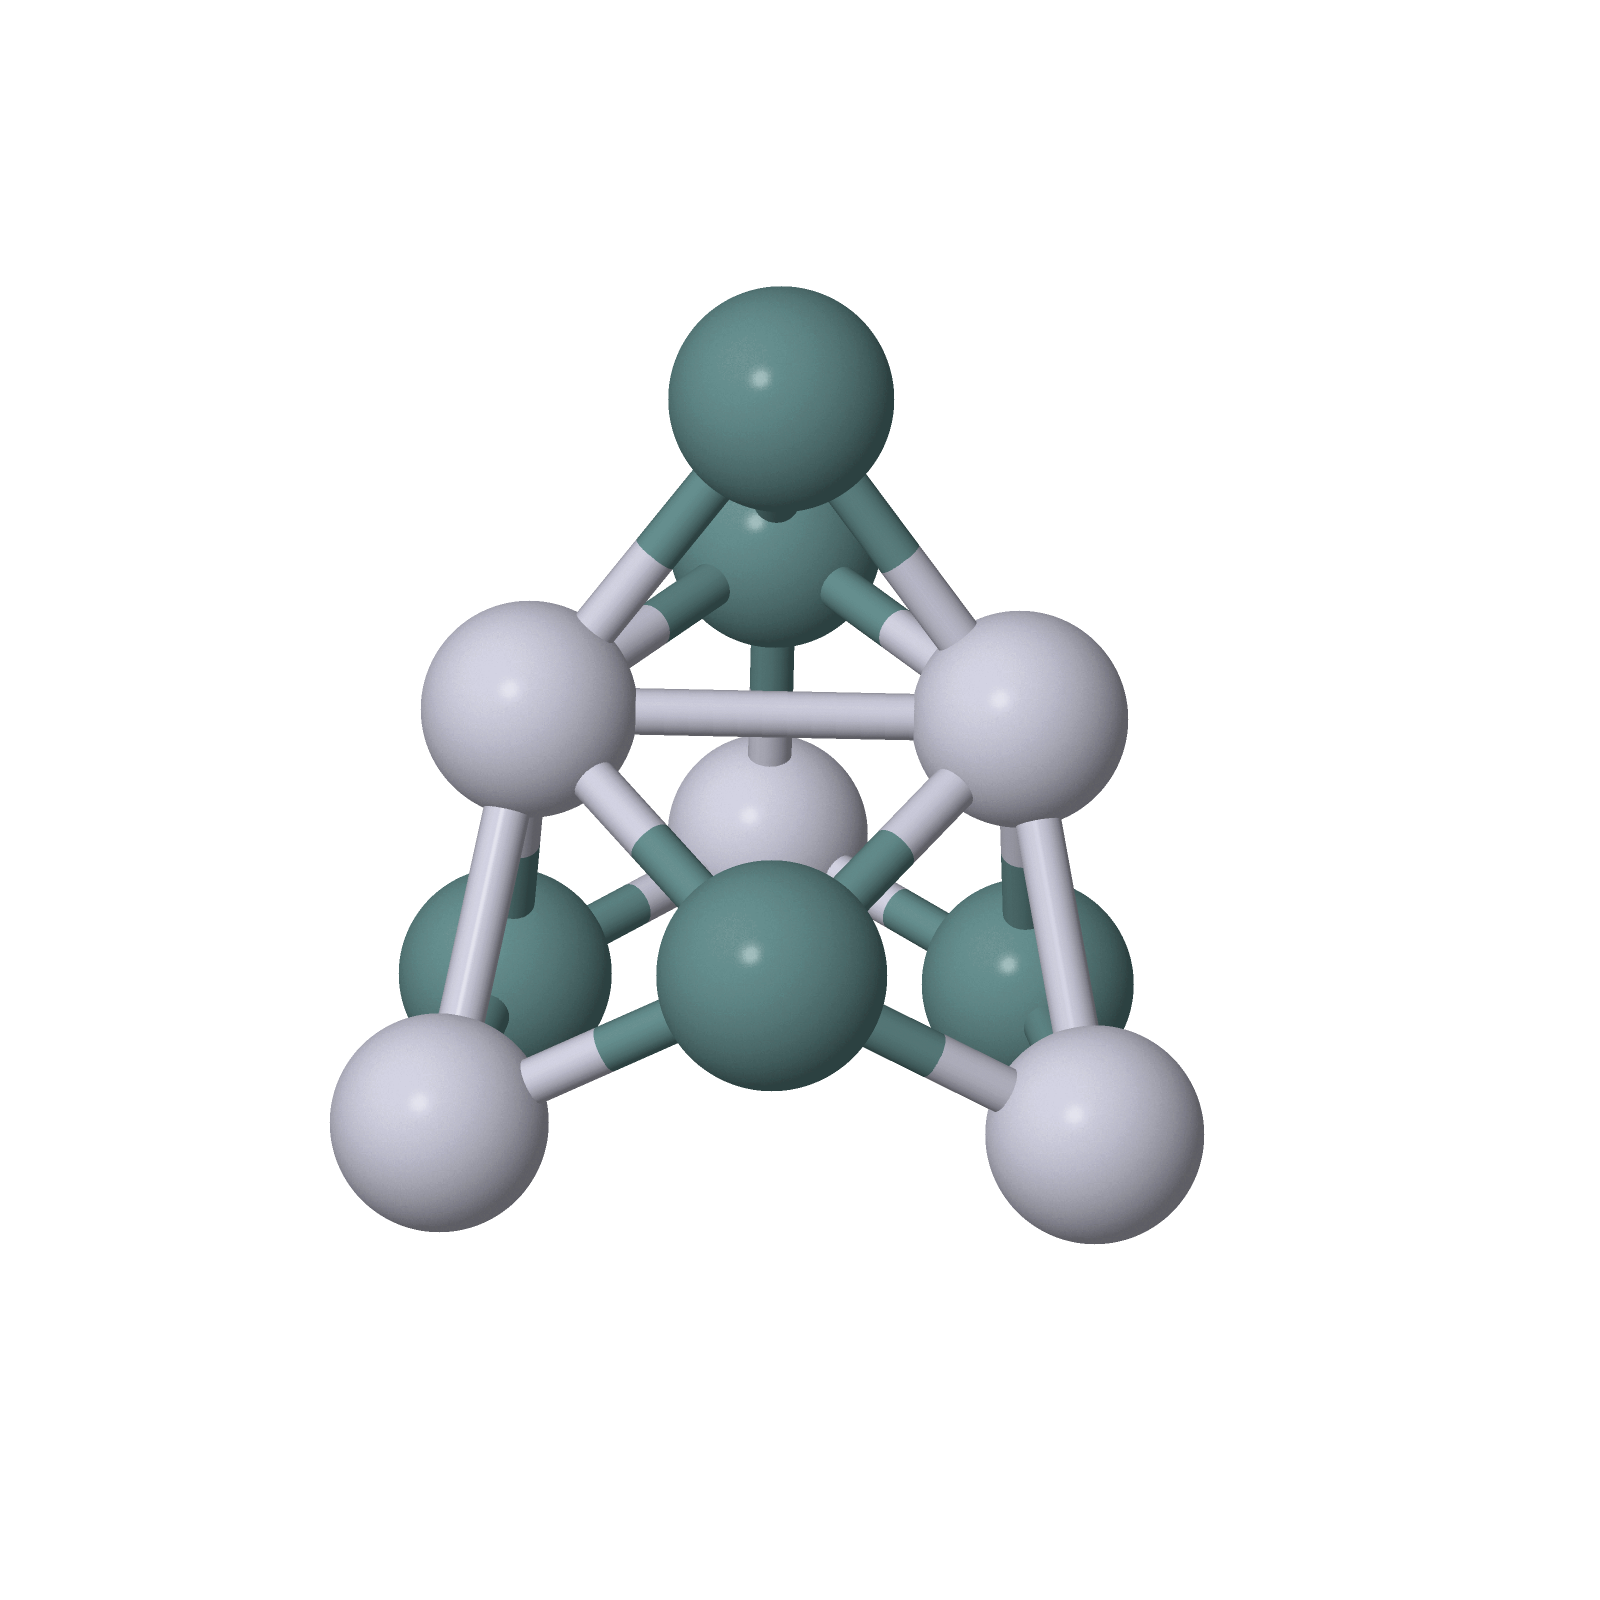
\includegraphics[width=\imgw]{Pt5Ge5_fromPt10Parent.png}};
\node[inner sep=0pt] (pt4ge6cross) at (\rightx,\bottomy)
  {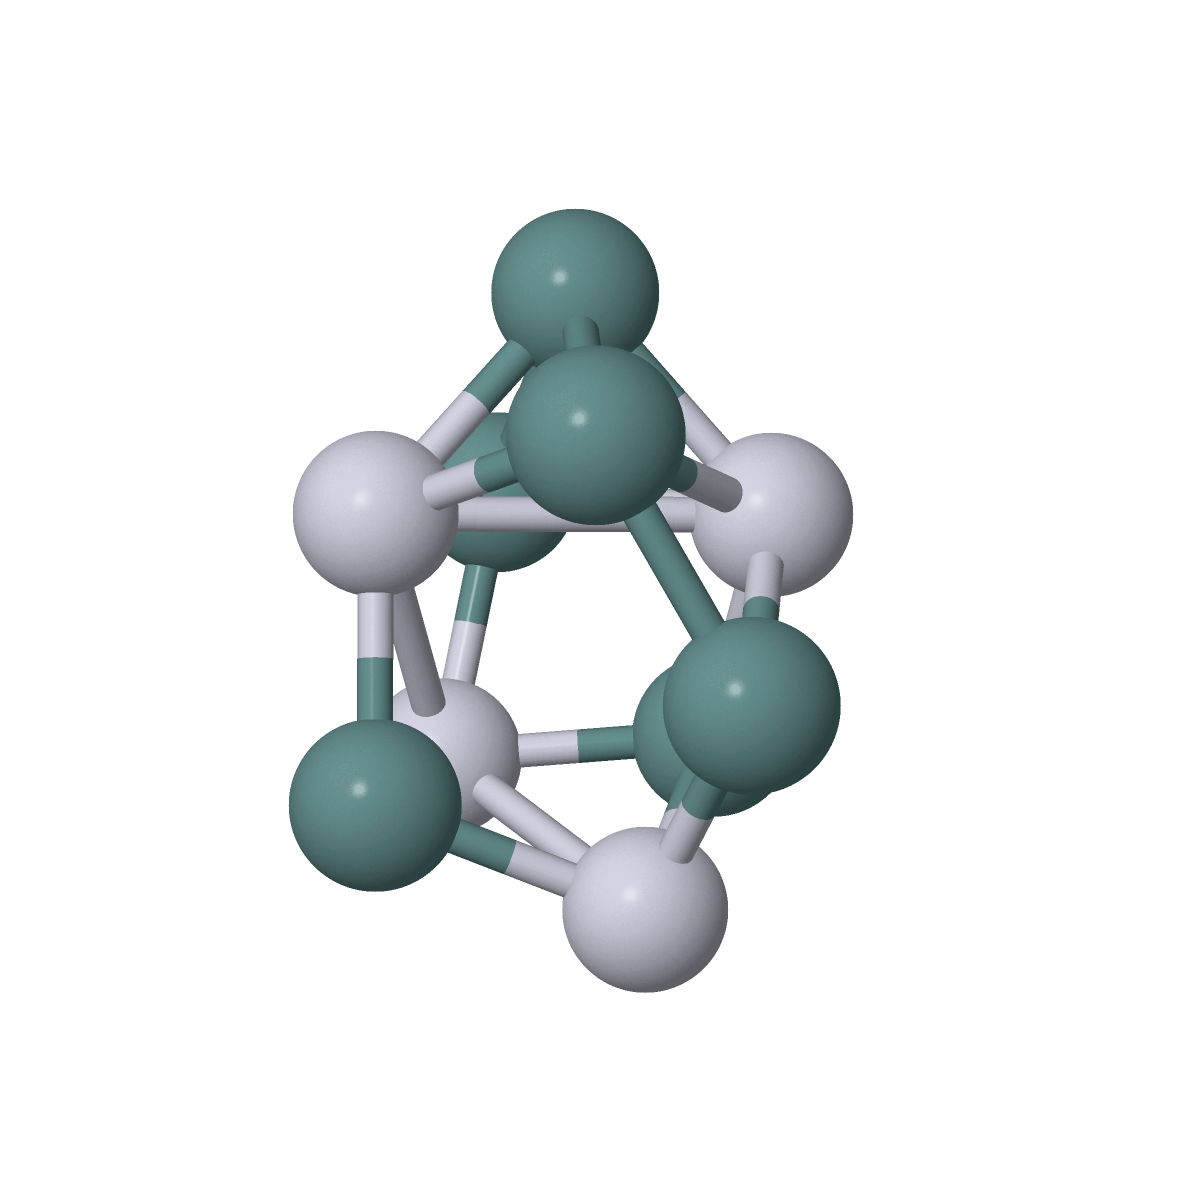
\includegraphics[width=\imgw]{pt4ge6.png}};

% Panel markers.
\node[panel] at ([xshift=-1.60cm,yshift=1.52cm]pt10cross.center) {(a)};
\node[panel] at ([xshift=-1.60cm,yshift=1.52cm]pt6ge4cross.center) {(b)};
\node[panel] at ([xshift=-1.60cm,yshift=1.52cm]pt5ge5cross.center) {(c)};
\node[panel] at ([xshift=-1.60cm,yshift=1.52cm]pt4ge6cross.center) {(d)};

% Model labels.
\node[title] at ([yshift=\titleshift]pt10cross.center)
  {\ce{Pt10} from \ce{Pt5Ge5}};
\node[title] at ([yshift=\titleshift]pt6ge4cross.center)
  {\ce{Pt6Ge4} from \ce{Pt10}};
\node[title] at ([yshift=\titleshift]pt5ge5cross.center)
  {\ce{Pt5Ge5} from \ce{Pt10}};
\node[title] at ([yshift=\titleshift]pt4ge6cross.center)
  {\ce{Pt4Ge6} from \ce{Pt10}};

% Pt10 site numbers.
\node[sitelabel] at ([xshift=-.10cm,yshift=-0.02cm]pt10cross.center) {1};
\node[sitelabel] at ([xshift=0.54cm,yshift=0.98cm]pt10cross.center) {3};
\node[sitelabel] at ([xshift=1.15cm,yshift=-0.25cm]pt10cross.center) {4};
\node[sitelabel] at ([xshift=1.18cm,yshift=0.33cm]pt10cross.center) {2};
\node[sitelabel] at ([xshift=-0.39cm,yshift=1.26cm]pt10cross.center) {10};
\node[sitelabel] at ([xshift=-1.30cm,yshift=0.66cm]pt10cross.center) {8};
\node[sitelabel] at ([xshift=-1.21cm,yshift=-0.33cm]pt10cross.center) {7};
\node[sitelabel] at ([xshift=-.53cm,yshift=-1.27cm]pt10cross.center) {6};
\node[sitelabel] at ([xshift=.66cm,yshift=-0.90cm]pt10cross.center) {5};
\node[sitelabel] at ([xshift=.12cm,yshift=.57cm]pt10cross.center) {9};

% Pt6Ge4 representative adsorption-site classes. Positions are tied to the
% selected Jmol view and can be fine-tuned independently.
\node[sitelabel] at ([xshift=-0.83cm,yshift=0.30cm]pt6ge4cross.center) {1};
\node[sitelabel] at ([xshift=-0.03cm,yshift=0.27cm]pt6ge4cross.center) {2};
\node[sitelabel] at ([xshift=0.82cm,yshift=0.32cm]pt6ge4cross.center) {4};
\node[sitelabel] at ([xshift=-0.02cm,yshift=-1.05cm]pt6ge4cross.center) {9};
\node[sitelabel] at ([xshift=-0.92cm,yshift=-1.1cm]pt6ge4cross.center) {7};
\node[sitelabel] at ([xshift=1.02cm,yshift=-1.05cm]pt6ge4cross.center) {5};

% Pt5Ge5 site-class numbers.
\node[sitelabel] at ([xshift=-.80cm,yshift=.30cm]pt5ge5cross.center) {6};
\node[sitelabel] at ([xshift=.68cm,yshift=.30cm]pt5ge5cross.center) {8};
\node[sitelabel] at ([xshift=-0.1cm,yshift=0.0cm]pt5ge5cross.center) {4};
\node[sitelabel] at ([xshift=-0.96cm,yshift=-0.85cm]pt5ge5cross.center) {7};
\node[sitelabel] at ([xshift=0.82cm,yshift=-0.85cm]pt5ge5cross.center) {10};

% Pt4Ge6 adsorption sites.
\node[sitelabel] at ([xshift=-0.80cm,yshift=0.39cm]pt4ge6cross.center) {1};
\node[sitelabel] at ([xshift=0.68cm,yshift=0.39cm]pt4ge6cross.center) {2};
\node[sitelabel] at ([xshift=-0.42cm,yshift=-0.46cm]pt4ge6cross.center) {5};
\node[sitelabel] at ([xshift=0.17cm,yshift=-1.08cm]pt4ge6cross.center) {7};

\end{tikzpicture}


\caption{Numbering of the Pt atoms used to place \ce{CO} and calculate the
\ce{CO} binding energies. Panel (a) shows the \ce{Pt10} model derived
from the \ce{Pt5Ge5} parent framework. Panels (b)--(d) show the \ce{Pt6Ge4},
\ce{Pt5Ge5}, and \ce{Pt4Ge6} derivatives,
respectively, generated from the \ce{Pt10} parent framework. The labels retain
the atom indices of the corresponding parent structure and identify the
starting adsorption sites.}
\label{fig:tfg_site_numbering}
\end{figure}


The ten triplet starting-site optimizations produce seven unique
\ce{Pt10CO} minima, which are collected in
Figure~\ref{fig:tfg_pt10co_series}. The paired labels 1/9, 3/5, and 8/10
indicate starting structures that converge to the same relaxed minimum. These
calculations provide a systematic set of trajectories from the selected
\ce{Pt10} isomer.

\begin{figure}[H]
\centering
\begin{tikzpicture}[
  x=1cm,
  y=1cm,
  structure/.style={inner sep=0pt},
  sitelabel/.style={font=\sffamily\scriptsize, align=center},
  datalabel/.style={font=\sffamily\tiny, align=center, text=black!75}
]

% Global layout controls.
\def\molw{0.22\linewidth}
\def\rowone{1.75}
\def\rowtwo{-1.75}
\def\xone{-4.35}
\def\xtwo{-1.45}
\def\xthree{1.45}
\def\xfour{4.35}
\def\labelshift{-1.48cm}
\def\datashift{-1.77cm}

% Seven unique minima obtained from the ten original TFG starting sites.
\node[structure] (site1) at (\xone,\rowone)
  {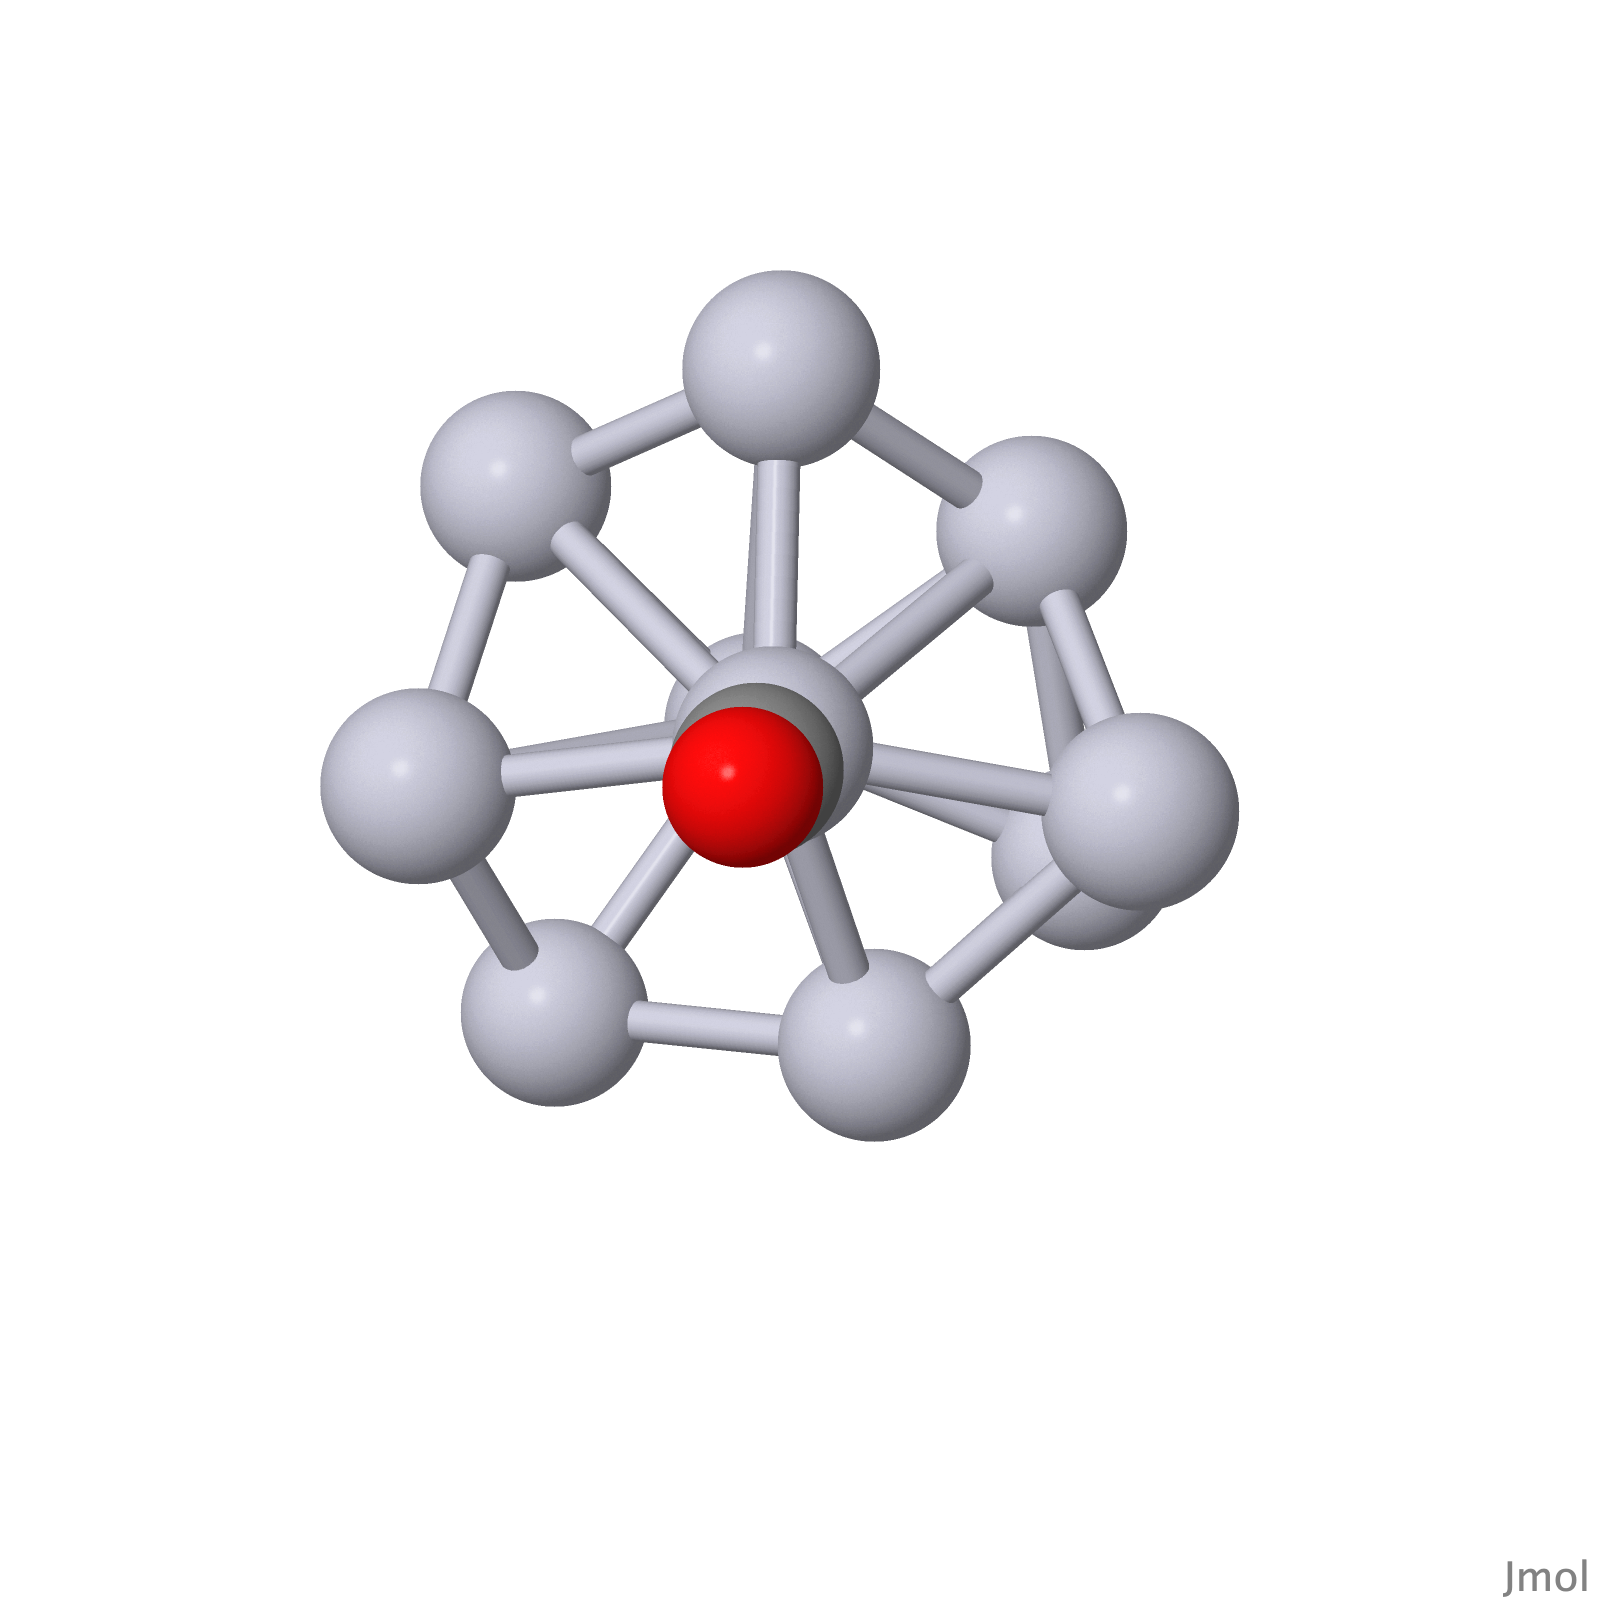
\includegraphics[width=\molw]{Pt10CO/Pt1_from_1xyzUnai.png}};
\node[structure] (site2) at (\xtwo,\rowone)
  {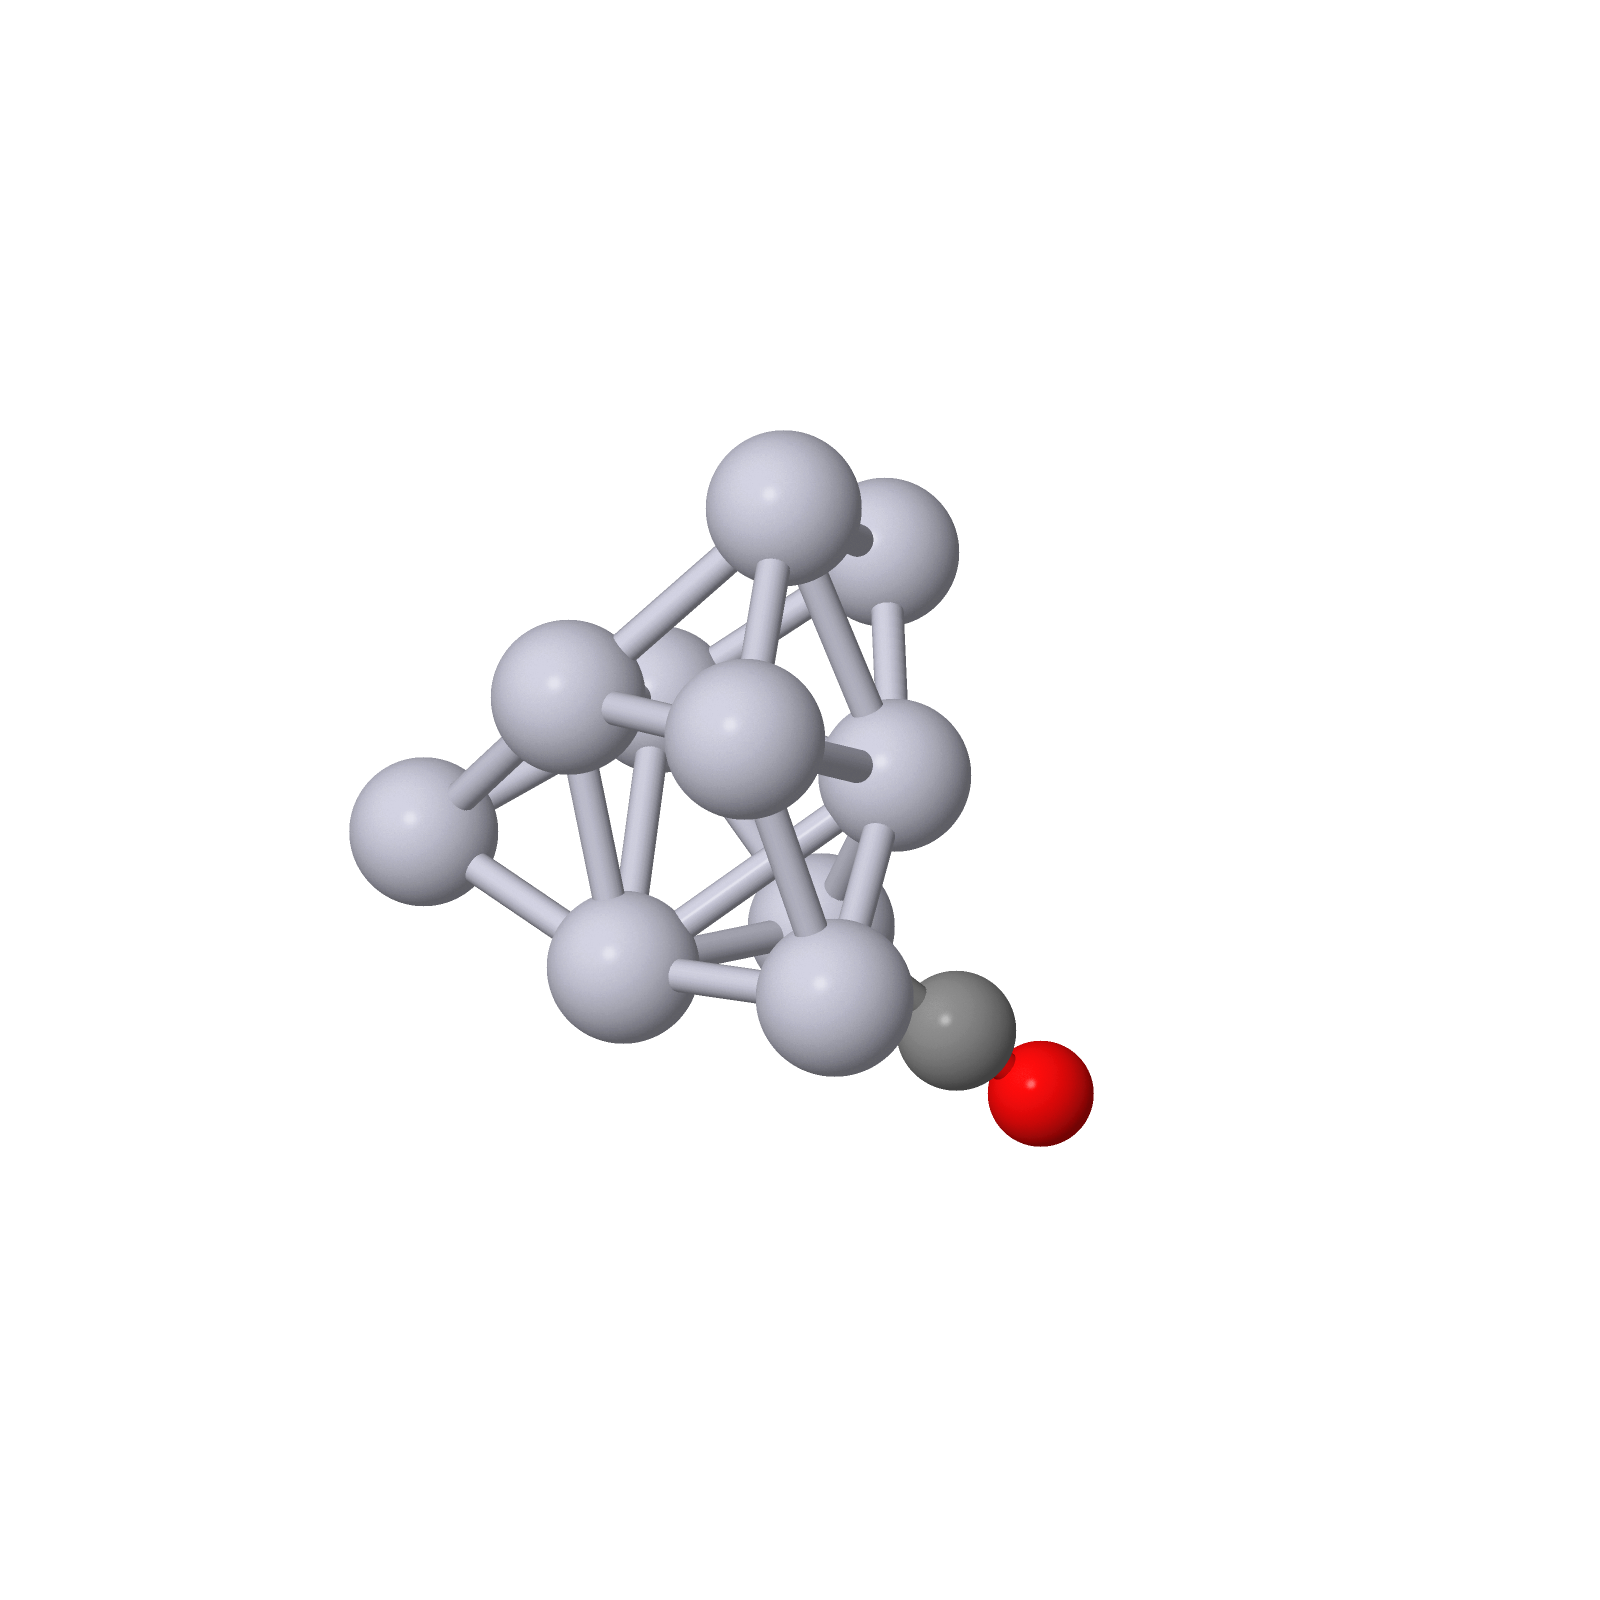
\includegraphics[width=\molw]{Pt10CO/Pt2_from_2xyzUnai.png}};
\node[structure] (site5) at (\xthree,\rowone)
  {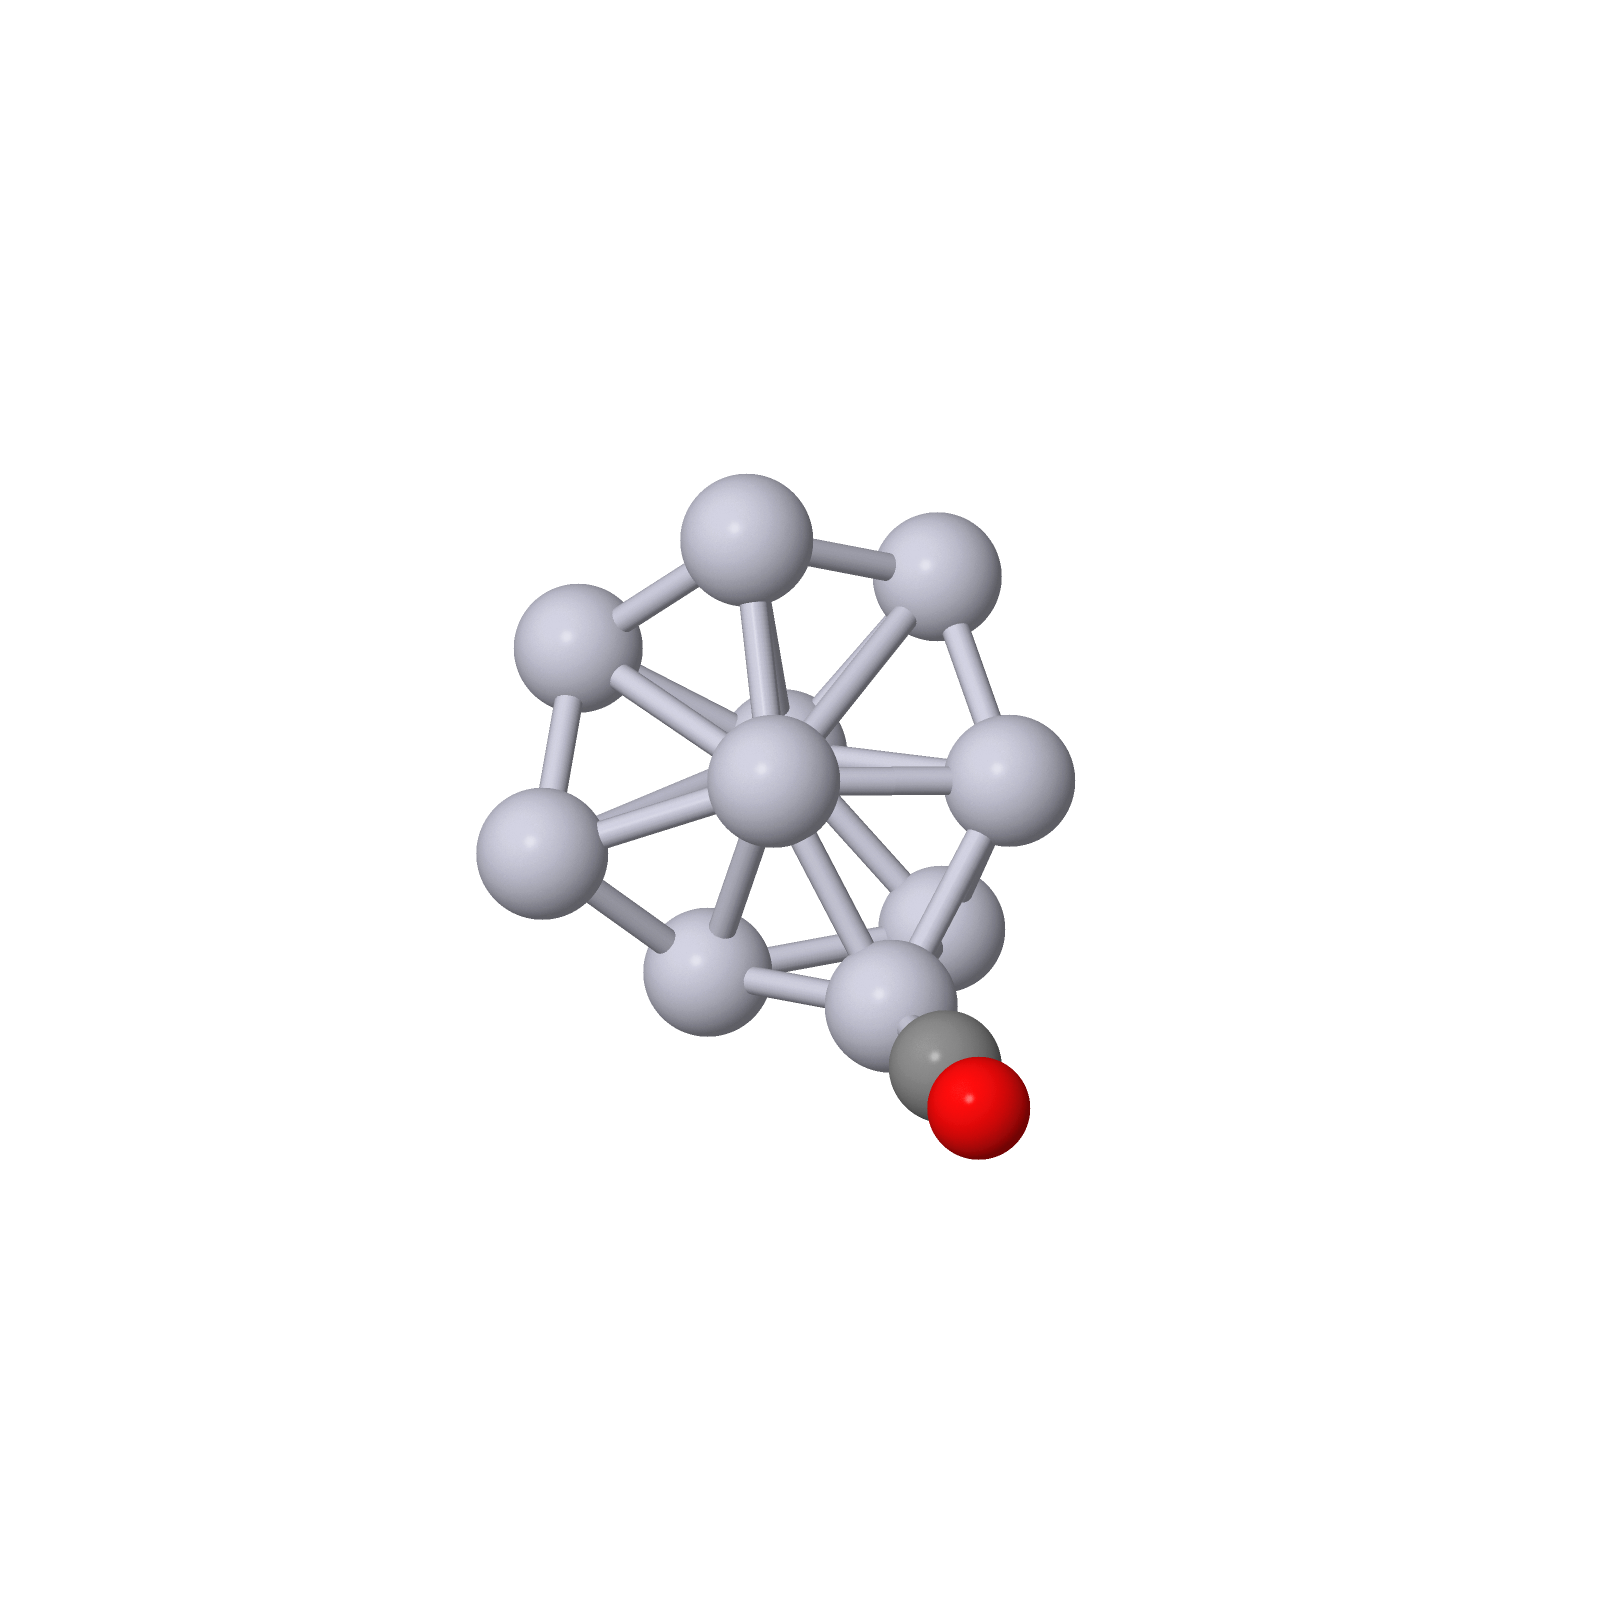
\includegraphics[width=\molw]{Pt10CO/Pt5_from_5xyzUnai.png}};
\node[structure] (site4) at (\xfour,\rowone)
  {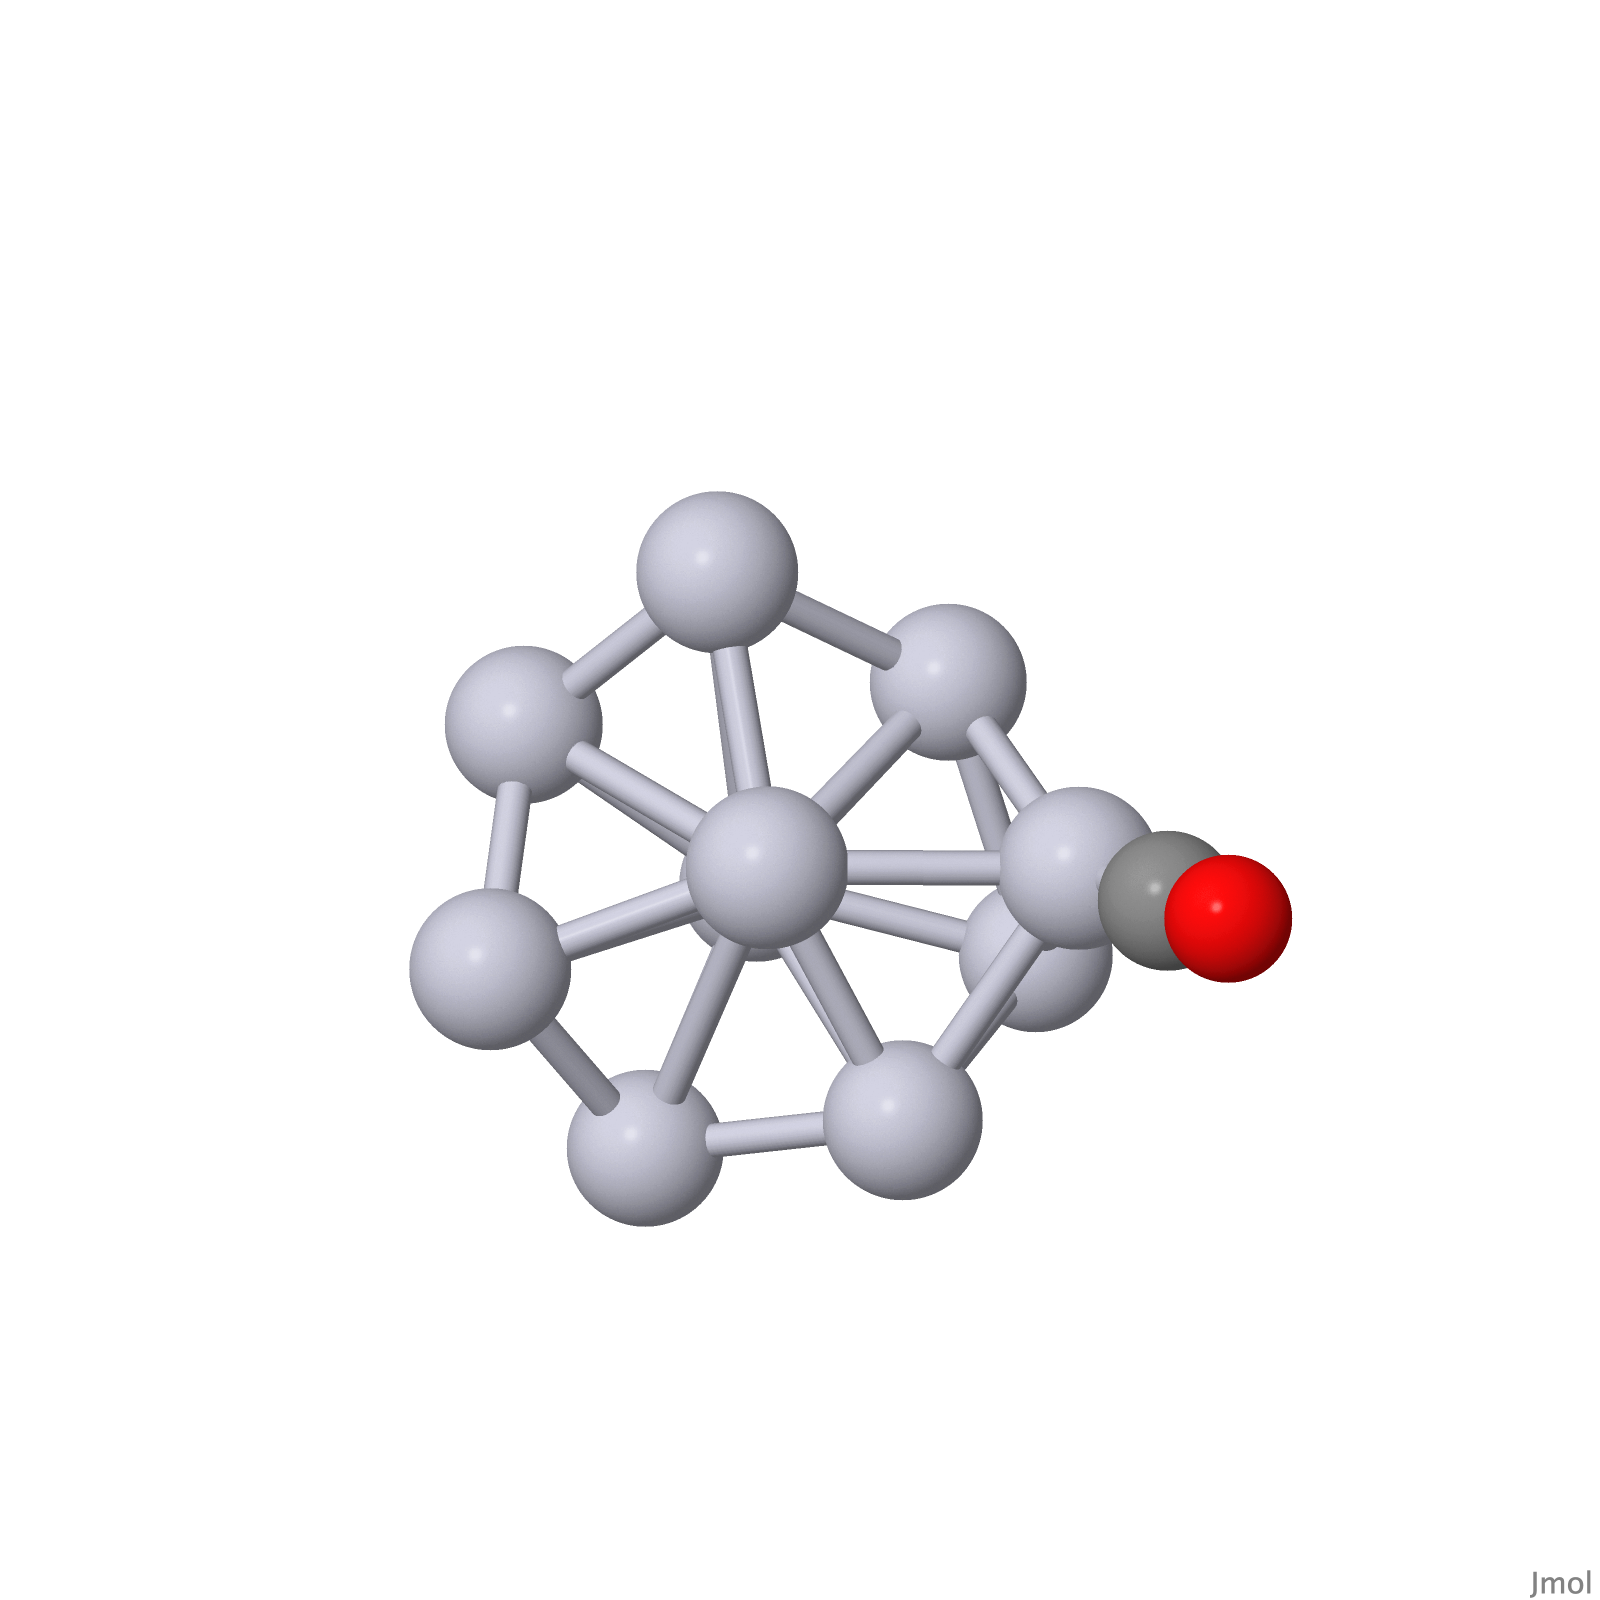
\includegraphics[width=\molw]{Pt10CO/pt4_from_4xyzUnai.png}};

\node[structure] (site6) at (-4.0,\rowtwo)
  {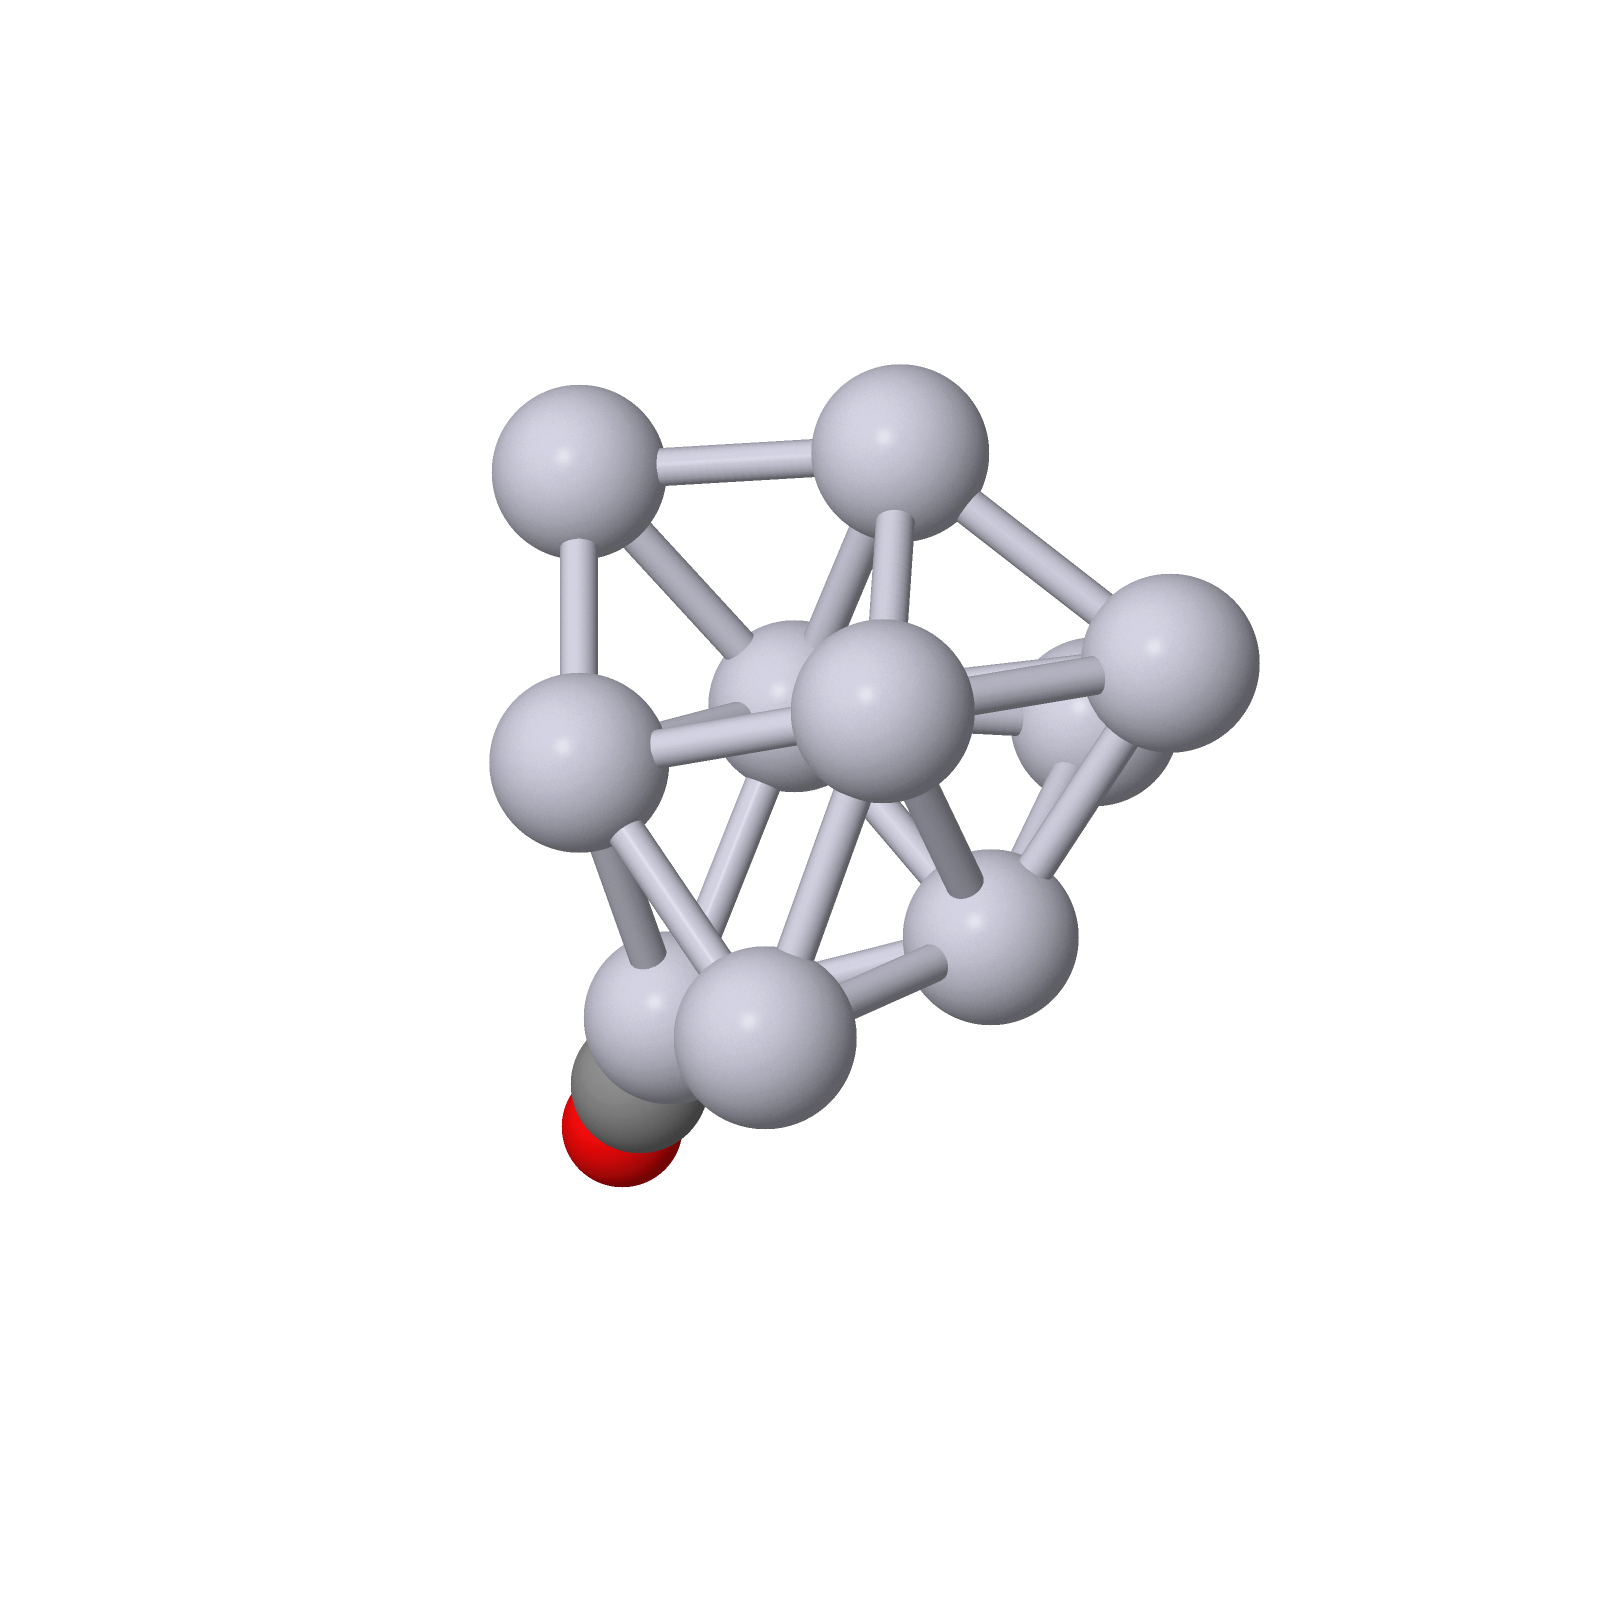
\includegraphics[width=\molw]{Pt10CO/Pt6_from_6xyzUnai.png}};
\node[structure] (site7) at (0,\rowtwo)
  {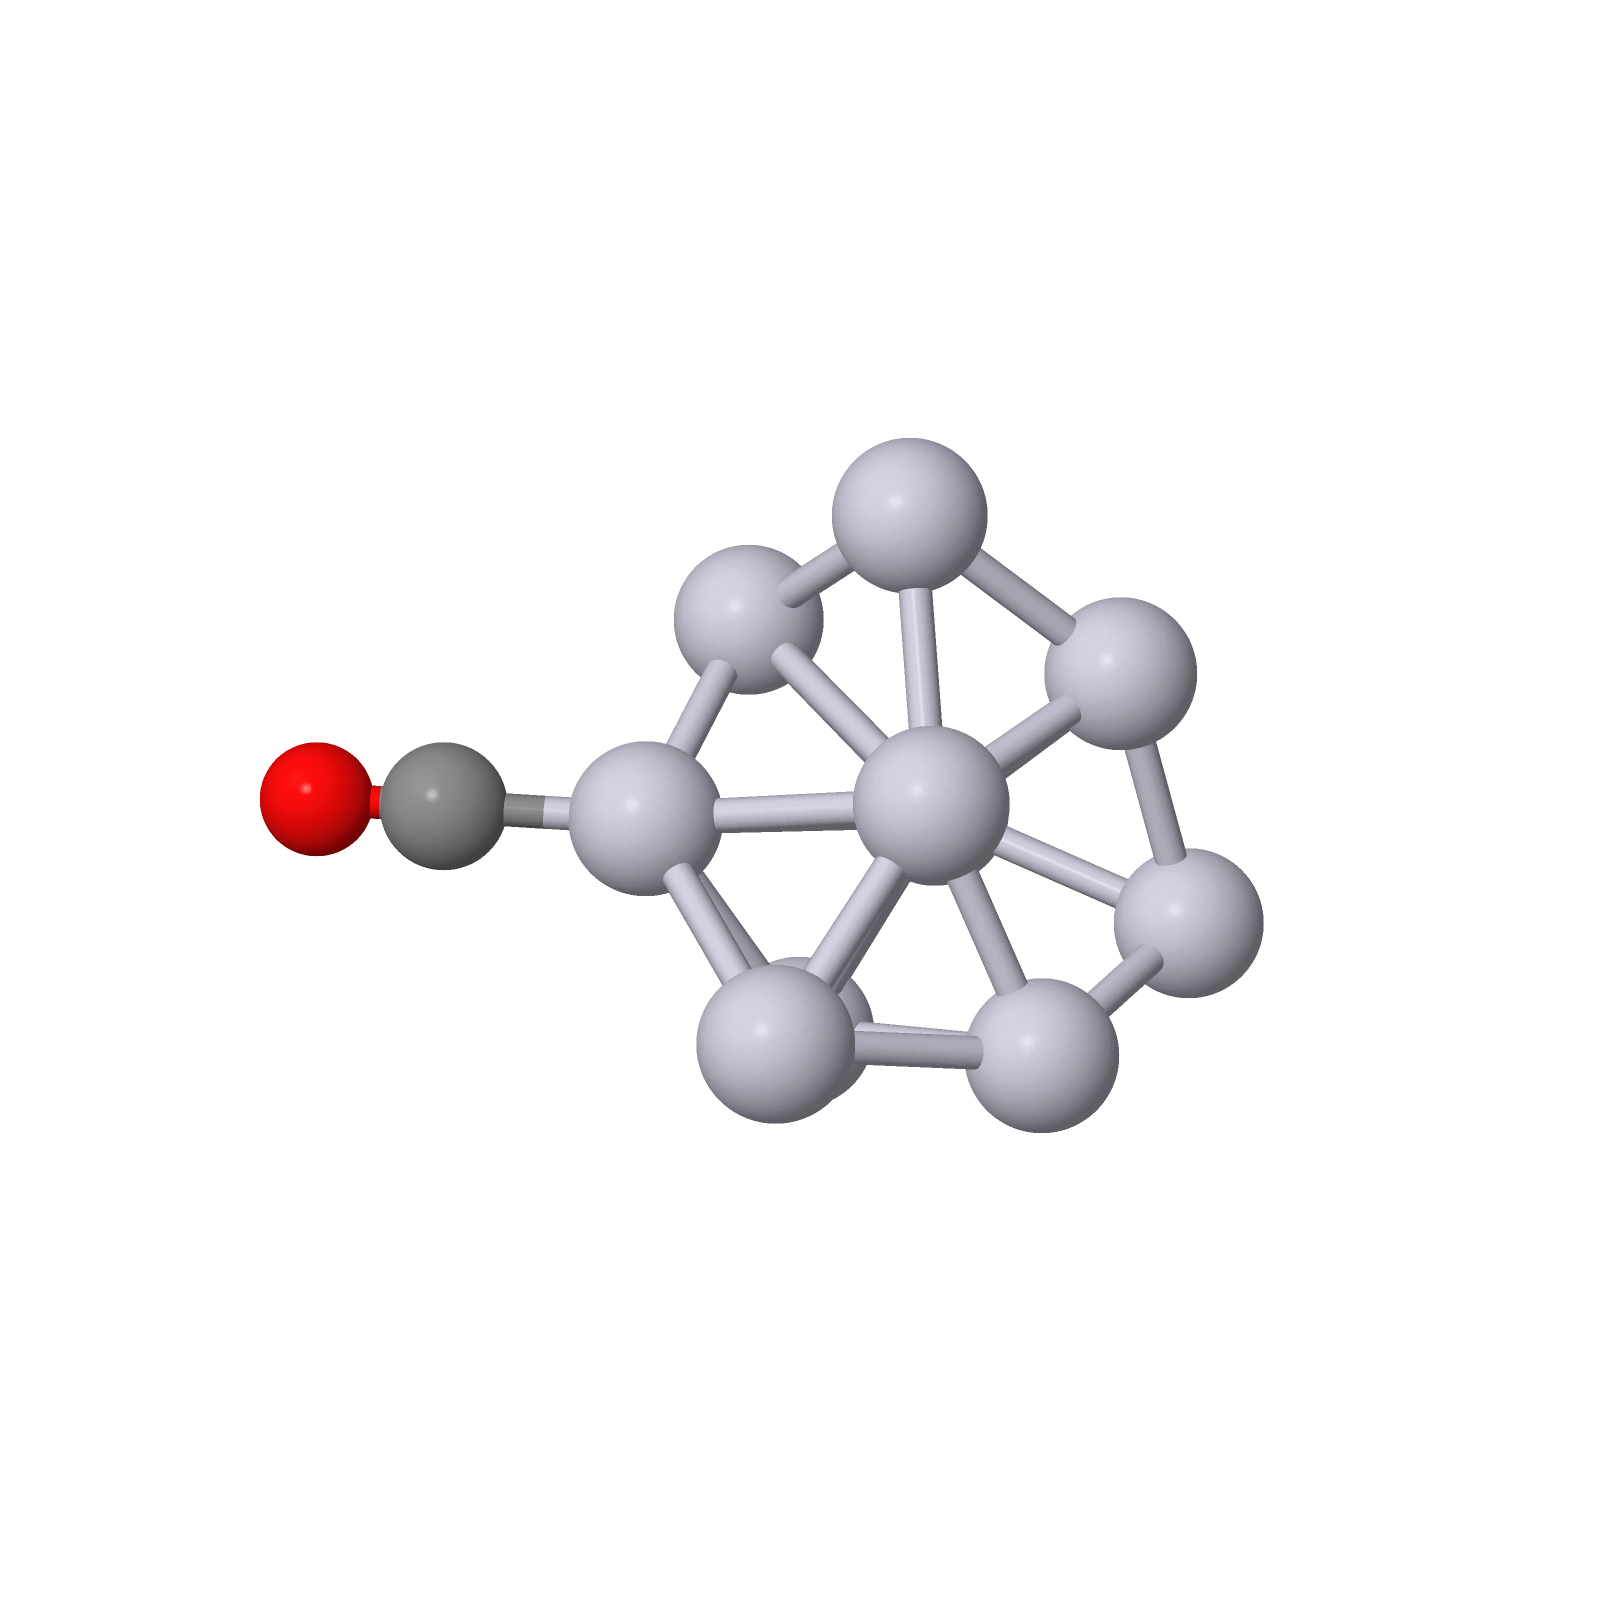
\includegraphics[width=\molw]{Pt10CO/Pt7_from_7xyzUnai.png}};
\node[structure] (site8) at (4.0,\rowtwo)
  {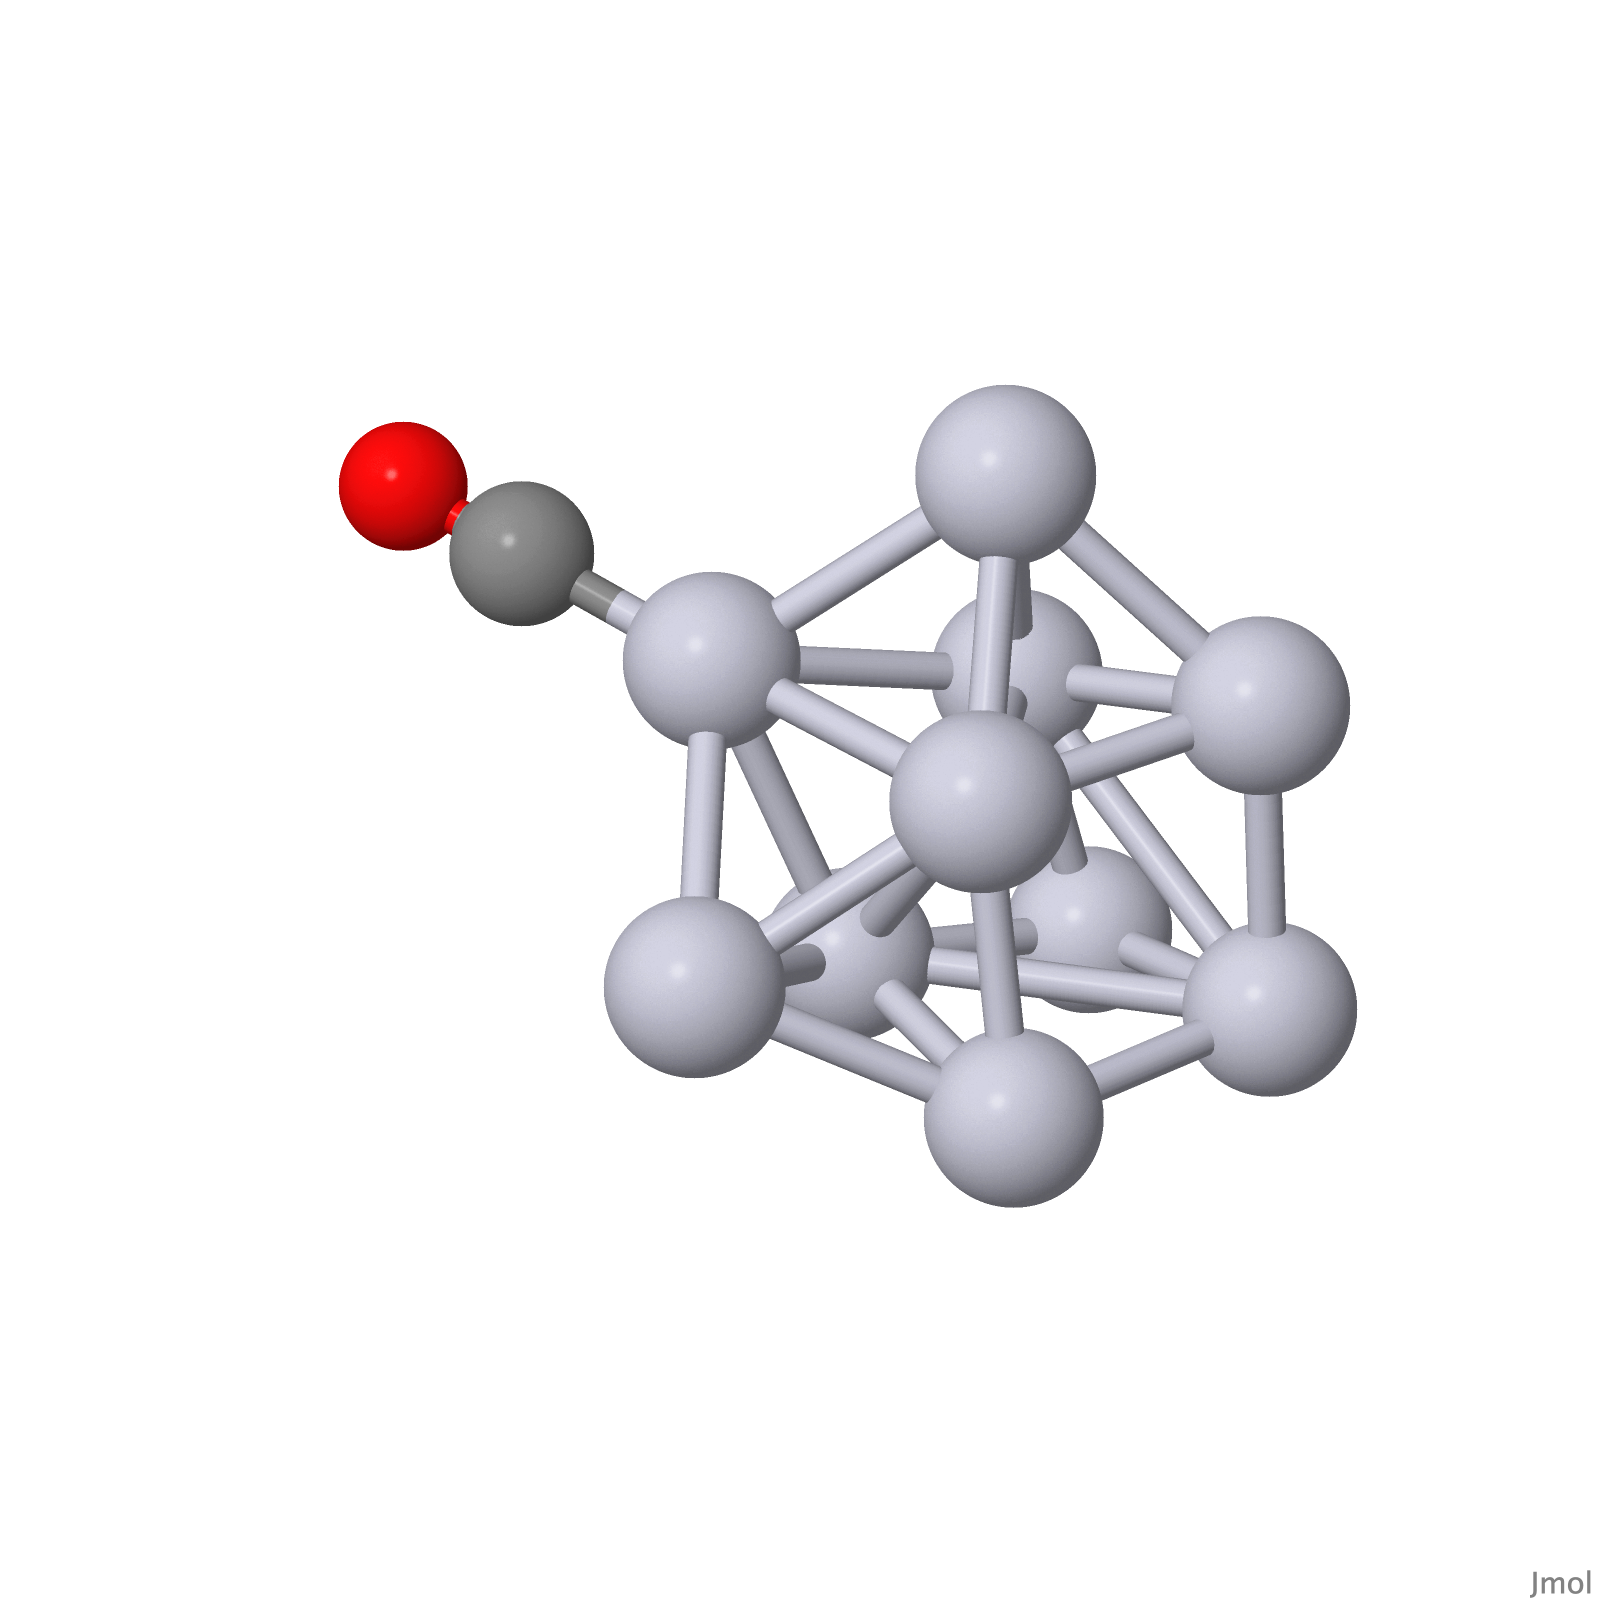
\includegraphics[width=\molw]{Pt10CO/Pt8_from_8xyzUnai.png}};

% Starting-site labels and binding energies of the final minima.
\node[sitelabel] at ([yshift=\labelshift]site1.center) {Sites 1/9};
\node[datalabel] at ([yshift=\datashift]site1.center) {$-2.156$ eV};
\node[sitelabel] at ([yshift=\labelshift]site2.center) {Site 2};
\node[datalabel] at ([yshift=\datashift]site2.center) {$-2.493$ eV};
\node[sitelabel] at ([yshift=\labelshift]site5.center) {Sites 3/5};
\node[datalabel] at ([yshift=\datashift]site5.center) {$-2.590$ eV};
\node[sitelabel] at ([yshift=\labelshift]site4.center) {Site 4};
\node[datalabel] at ([yshift=\datashift]site4.center) {$-2.579$ eV};

\node[sitelabel] at ([yshift=\labelshift]site6.center) {Site 6};
\node[datalabel] at ([yshift=\datashift]site6.center) {$-2.657$ eV};
\node[sitelabel] at ([yshift=\labelshift]site7.center) {Site 7};
\node[datalabel] at ([yshift=\datashift]site7.center) {$-2.493$ eV};
\node[sitelabel] at ([yshift=\labelshift]site8.center) {Sites 8/10};
\node[datalabel] at ([yshift=\datashift]site8.center) {$-2.650$ eV};

\end{tikzpicture}

\caption{Seven unique optimized triplet \ce{Pt10CO} minima obtained from the
ten initial Pt adsorption sites of the \ce{Pt10} derivative. Site
labels follow Figure~\ref{fig:tfg_site_numbering}; paired labels identify
initial structures that converge to the same final minimum. The corresponding
triplet $BE(\ce{CO})$ values are given below each structure. {The
analogous quintet calculations produced five distinct minima; their relative
and binding energies are also reported together with the triplet results in
Table~\ref{tab:tfg_adsorption_descriptors}.}}
\label{fig:tfg_pt10co_series}
\end{figure}

The optimized carbonyl structures of the three Ge-containing compositions are
shown in Figure~\ref{fig:tfg_ptgeco_series}.

\begin{figure}[H]
\centering
\begin{tikzpicture}[
  x=1cm,
  y=1cm,
  structure/.style={inner sep=0pt},
  rowlabel/.style={font=\sffamily\small\bfseries, align=center},
  sitelabel/.style={font=\sffamily\scriptsize, align=center},
  datalabel/.style={font=\sffamily\tiny, align=center, text=black!75}
]

% Global layout controls.
\def\molwA{0.17\linewidth}
\def\molwB{0.13\linewidth}
\def\molwC{0.15\linewidth}
\def\molw{0.215\linewidth}
\def\rowone{3.55}
\def\rowtwo{0.00}
\def\rowthree{-3.55}
\def\xone{-4.65}
\def\xtwo{-1.55}
\def\xthree{1.55}
\def\xfour{4.65}
\def\xmidleft{-3.10}
\def\xmid{0.00}
\def\xmidright{3.10}
\def\labelshift{-1.47cm}
\def\datashift{-1.73cm}

% Pt6Ge4CO adsorption sites.
\node[structure] (p6g4s1) at (\xone,\rowone)
  {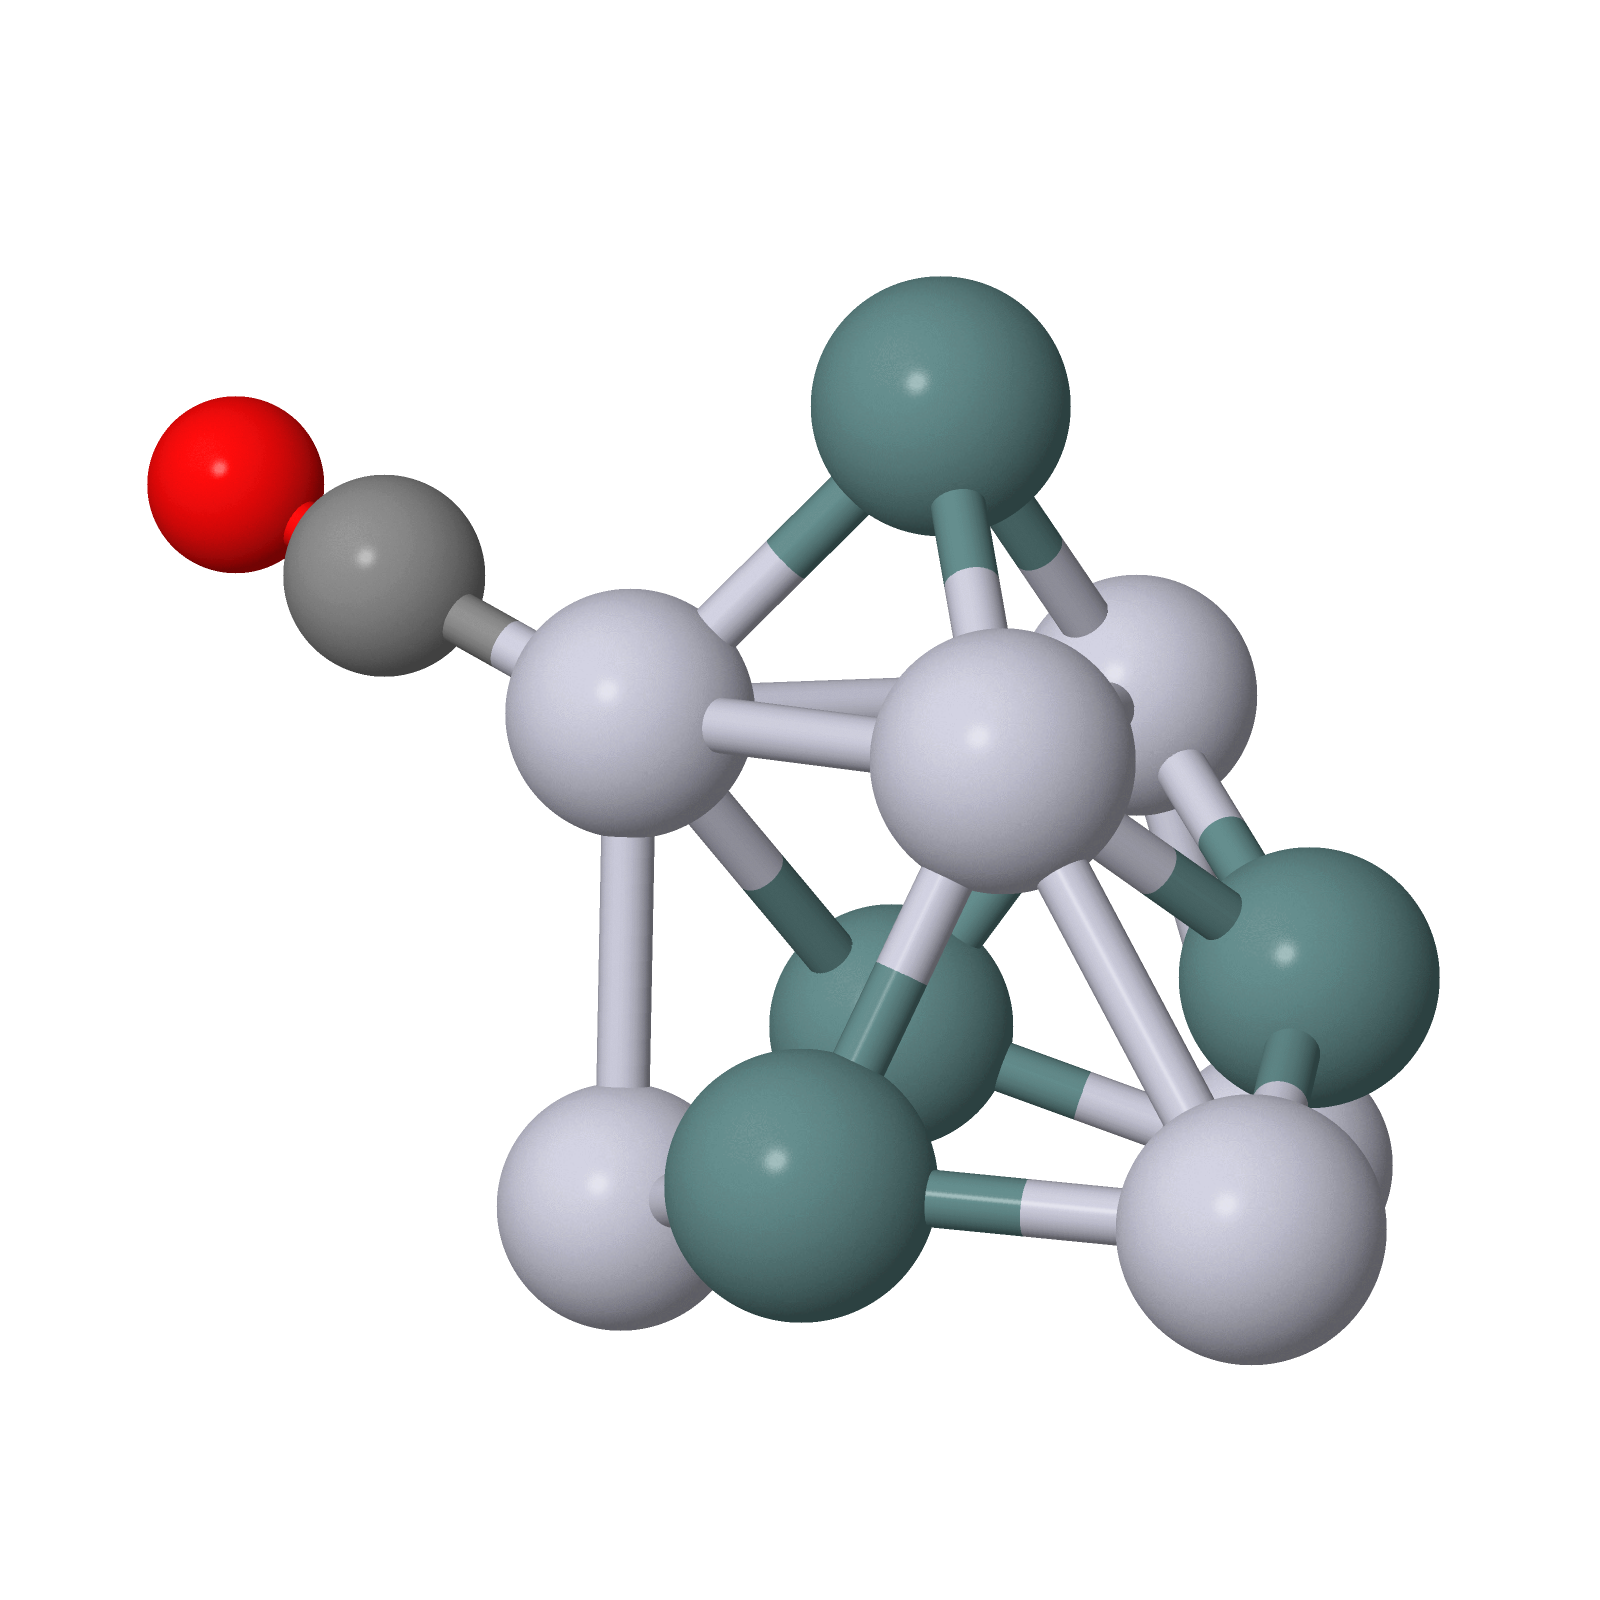
\includegraphics[width=\molwB]{pt6ge4_site01.png}};
\node[structure] (p6g4s2) at (\xtwo,\rowone)
  {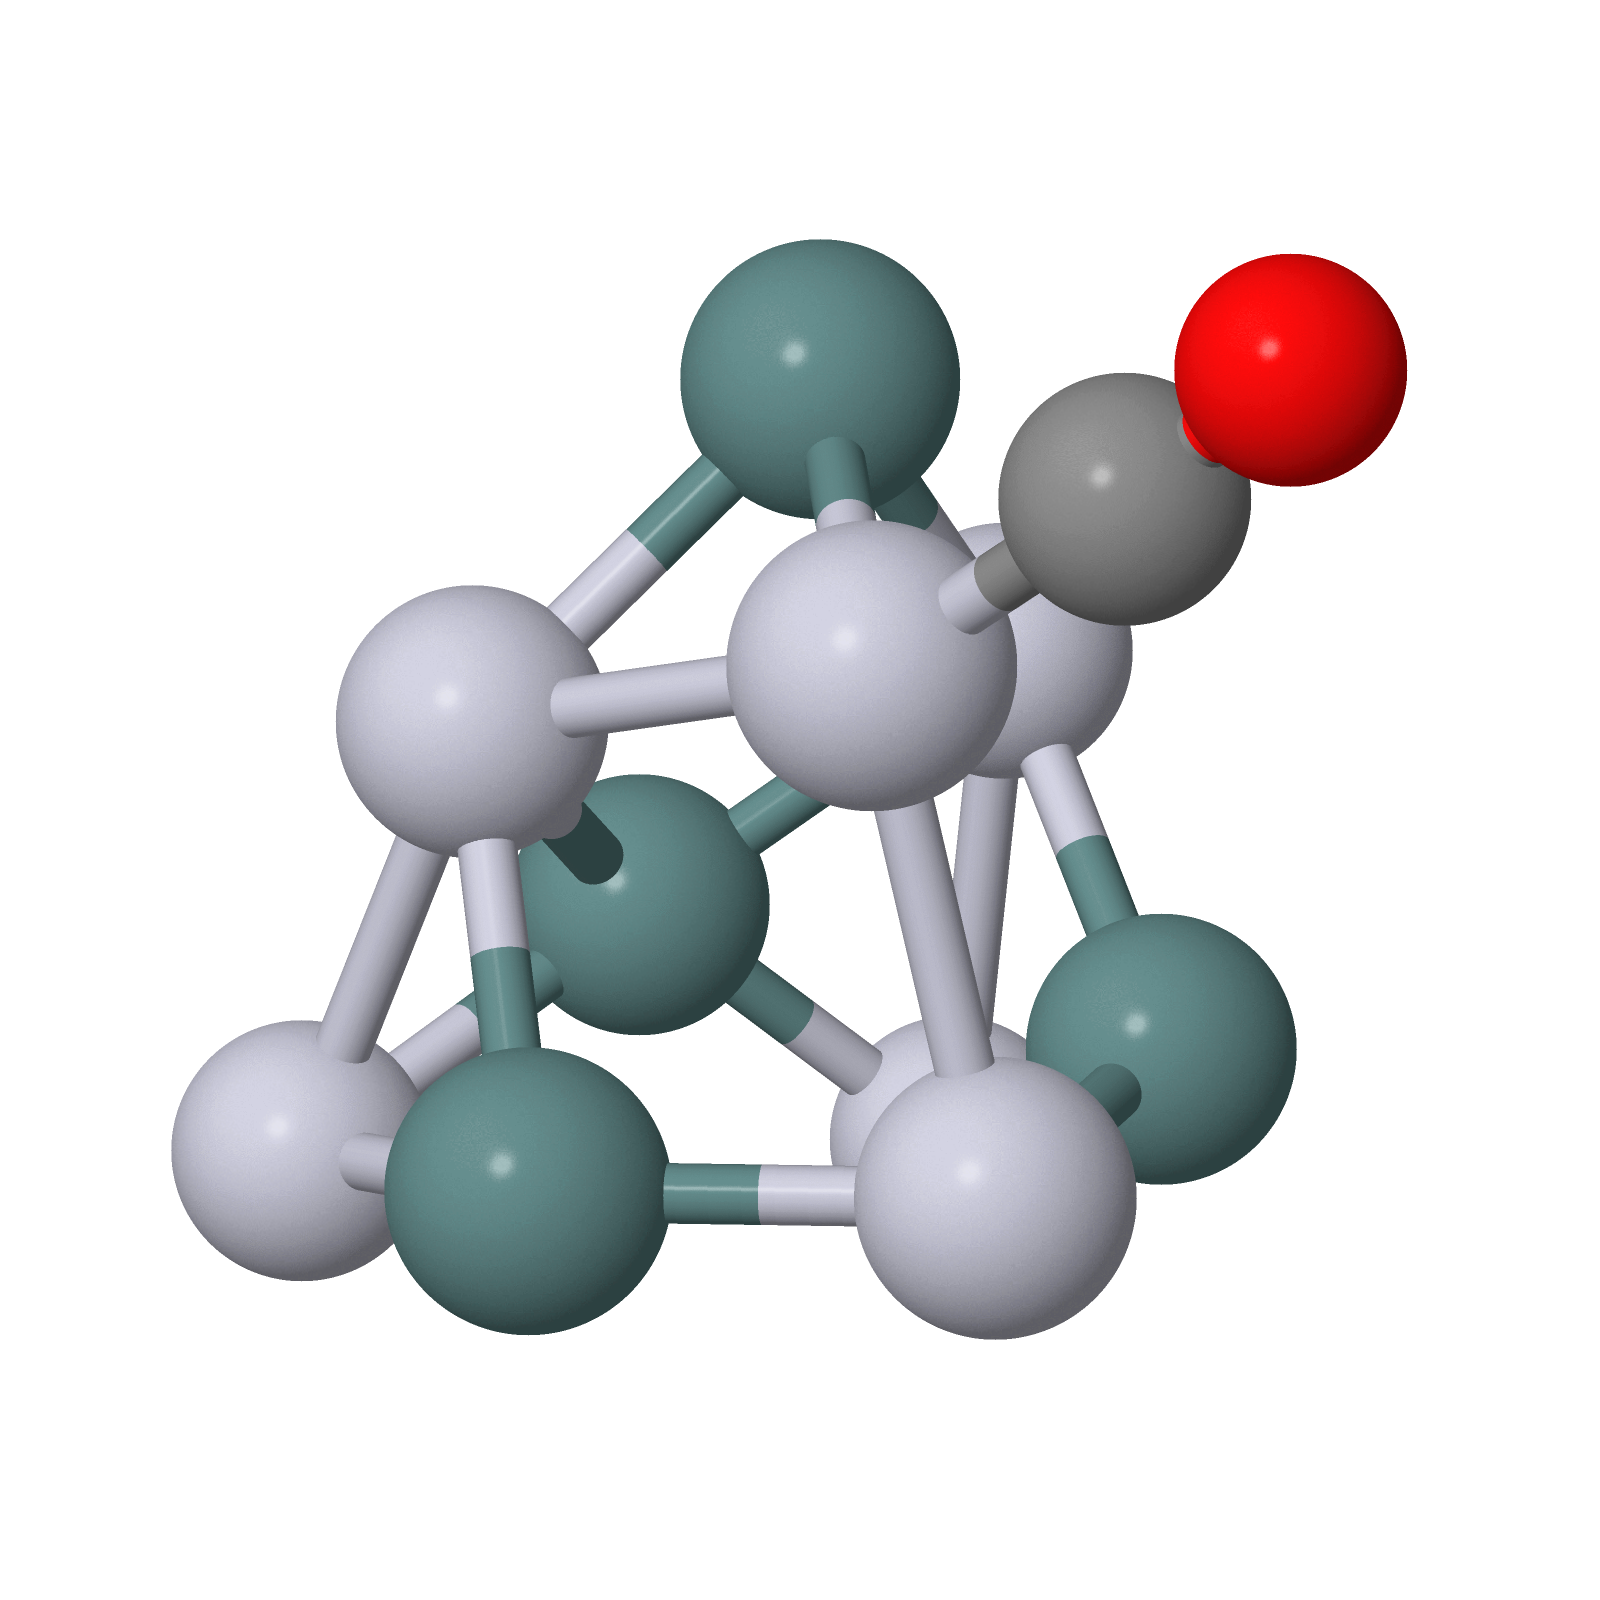
\includegraphics[width=\molwB]{pt6ge4_site02.png}};
\node[structure] (p6g4s7) at (\xthree,\rowone)
  {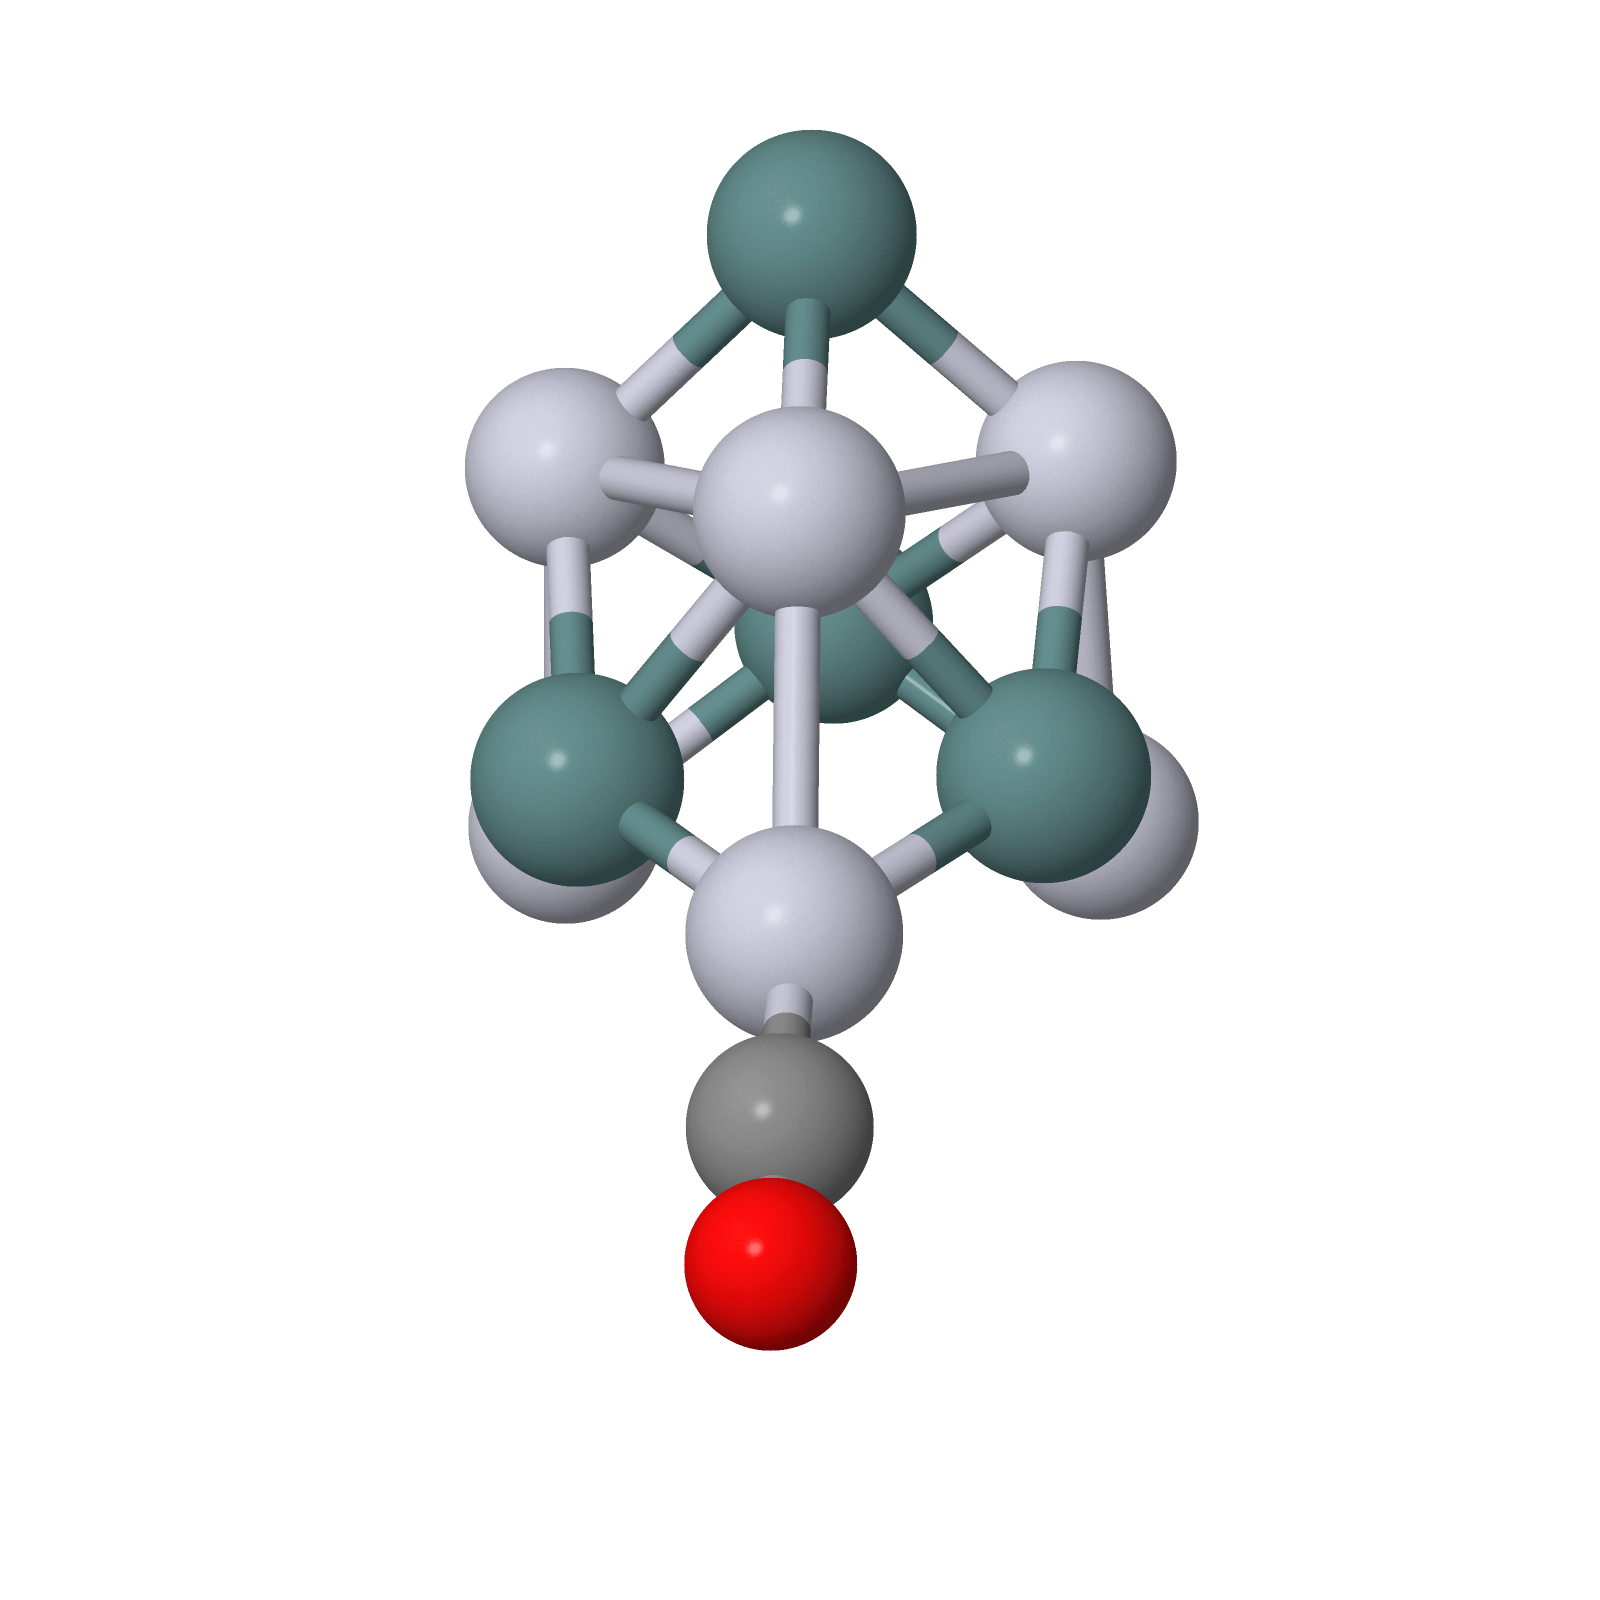
\includegraphics[width=\molwA]{pt6ge4_site07.png}};
\node[structure] (p6g4s9) at (\xfour,\rowone)
  {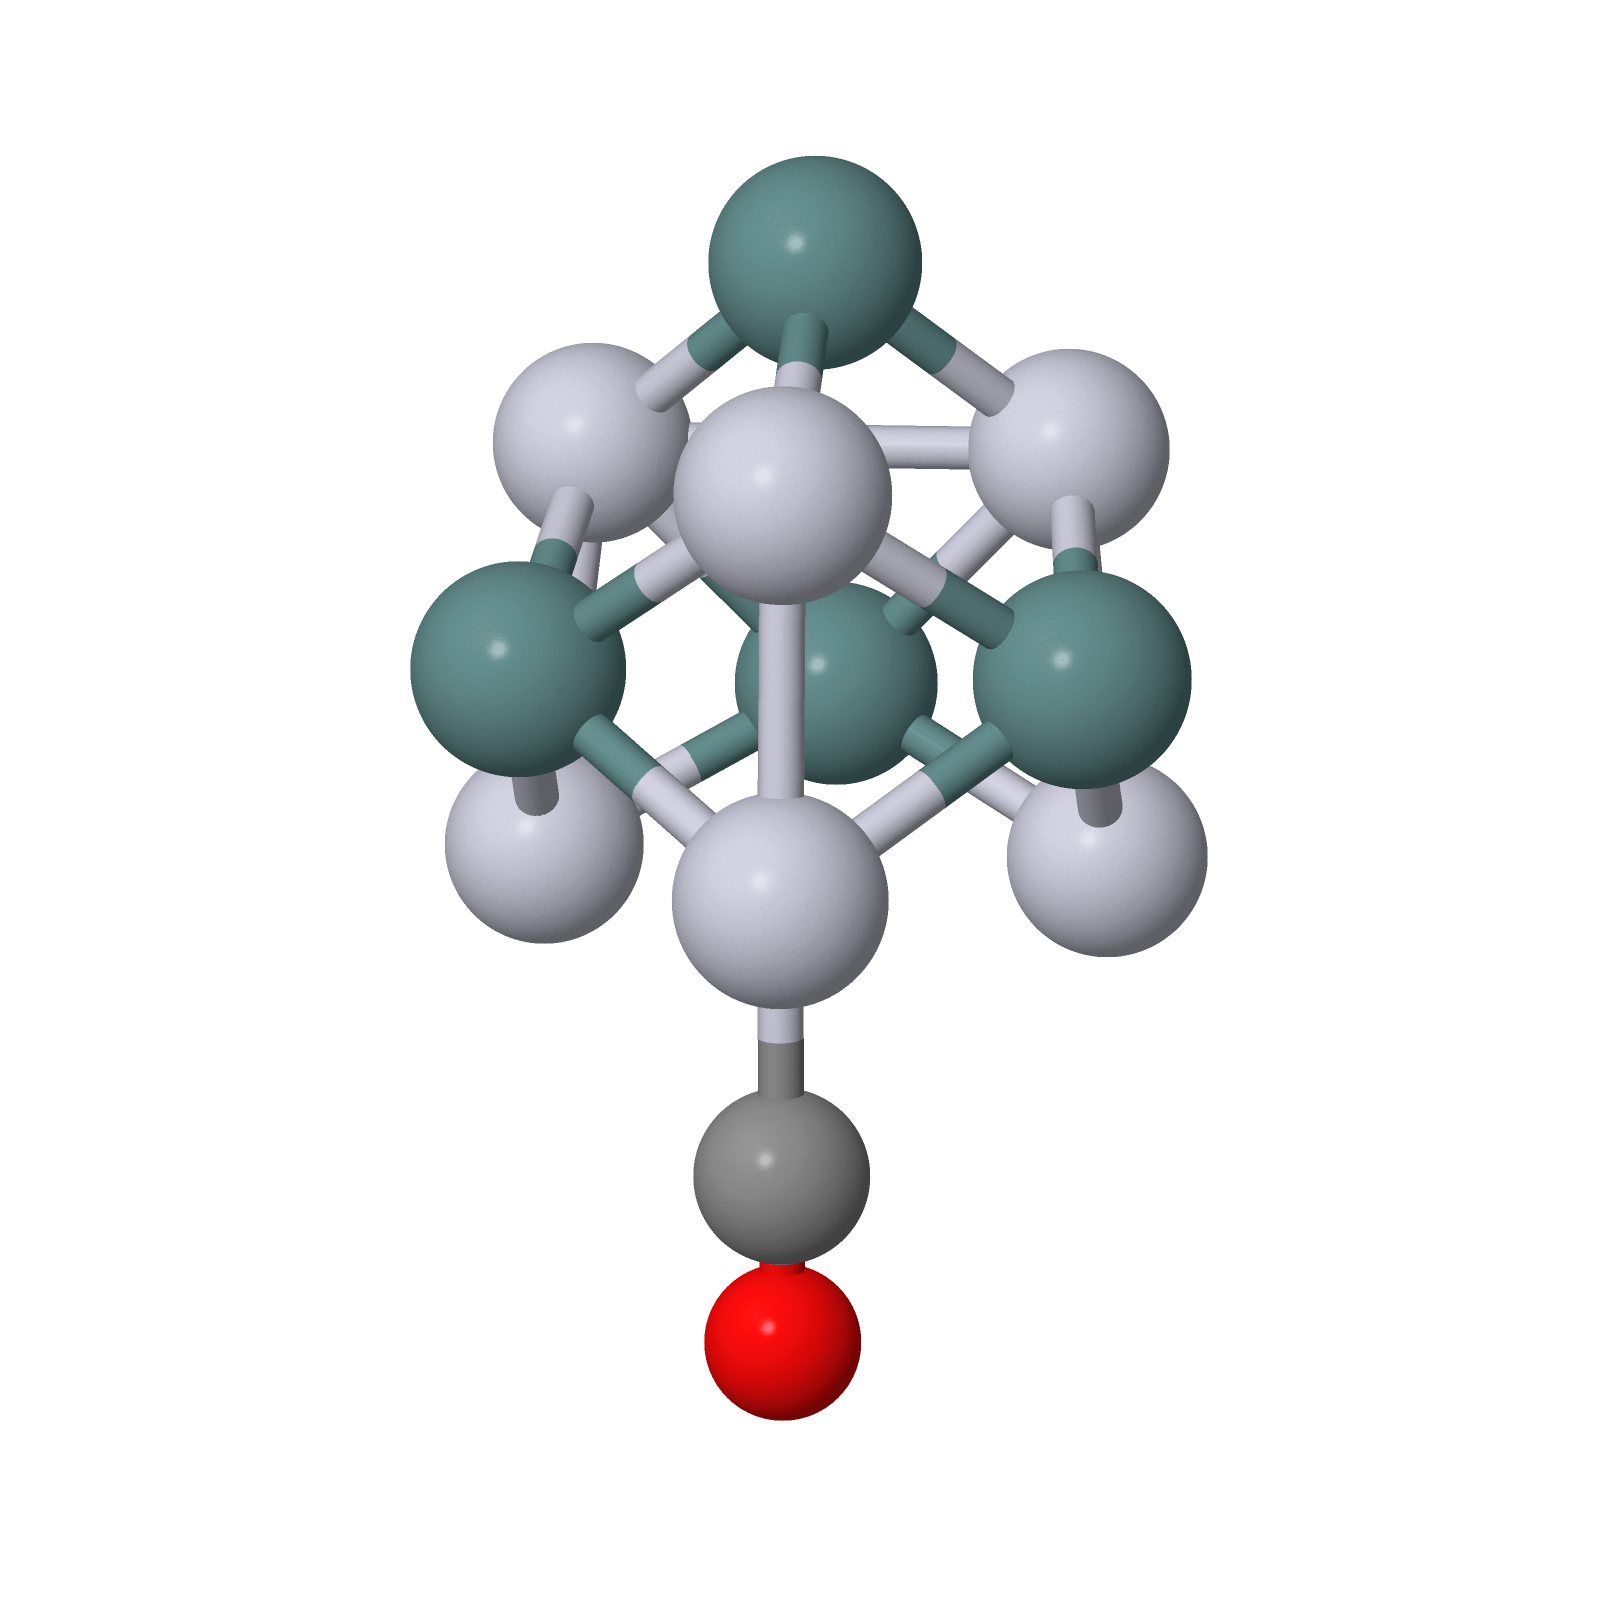
\includegraphics[width=\molwA]{pt6ge4_site09.png}};

\node[rowlabel] at (0,{\rowone+1.48}) {\ce{Pt6Ge4CO}};
\node[sitelabel] at ([yshift=\labelshift]p6g4s1.center) {Site 1/4};
\node[datalabel] at ([yshift=\datashift]p6g4s1.center) {$-2.235$ eV};
\node[sitelabel] at ([yshift=\labelshift]p6g4s2.center) {Site 2};
\node[datalabel] at ([yshift=\datashift]p6g4s2.center) {$-2.246$ eV};
\node[sitelabel] at ([yshift=\labelshift]p6g4s7.center) {Site 5/7};
\node[datalabel] at ([yshift=\datashift]p6g4s7.center) {$-1.567$ eV};
\node[sitelabel] at ([yshift=\labelshift]p6g4s9.center) {Site 9};
\node[datalabel] at ([yshift=\datashift]p6g4s9.center) {$-2.245$ eV};

% Pt5Ge5CO adsorption-site classes. Parent-Pt indices are retained; paired
% labels denote equivalent sites represented by the same optimized structure.
\node[structure] (p5g5s1) at (\xmidleft,\rowtwo)
  {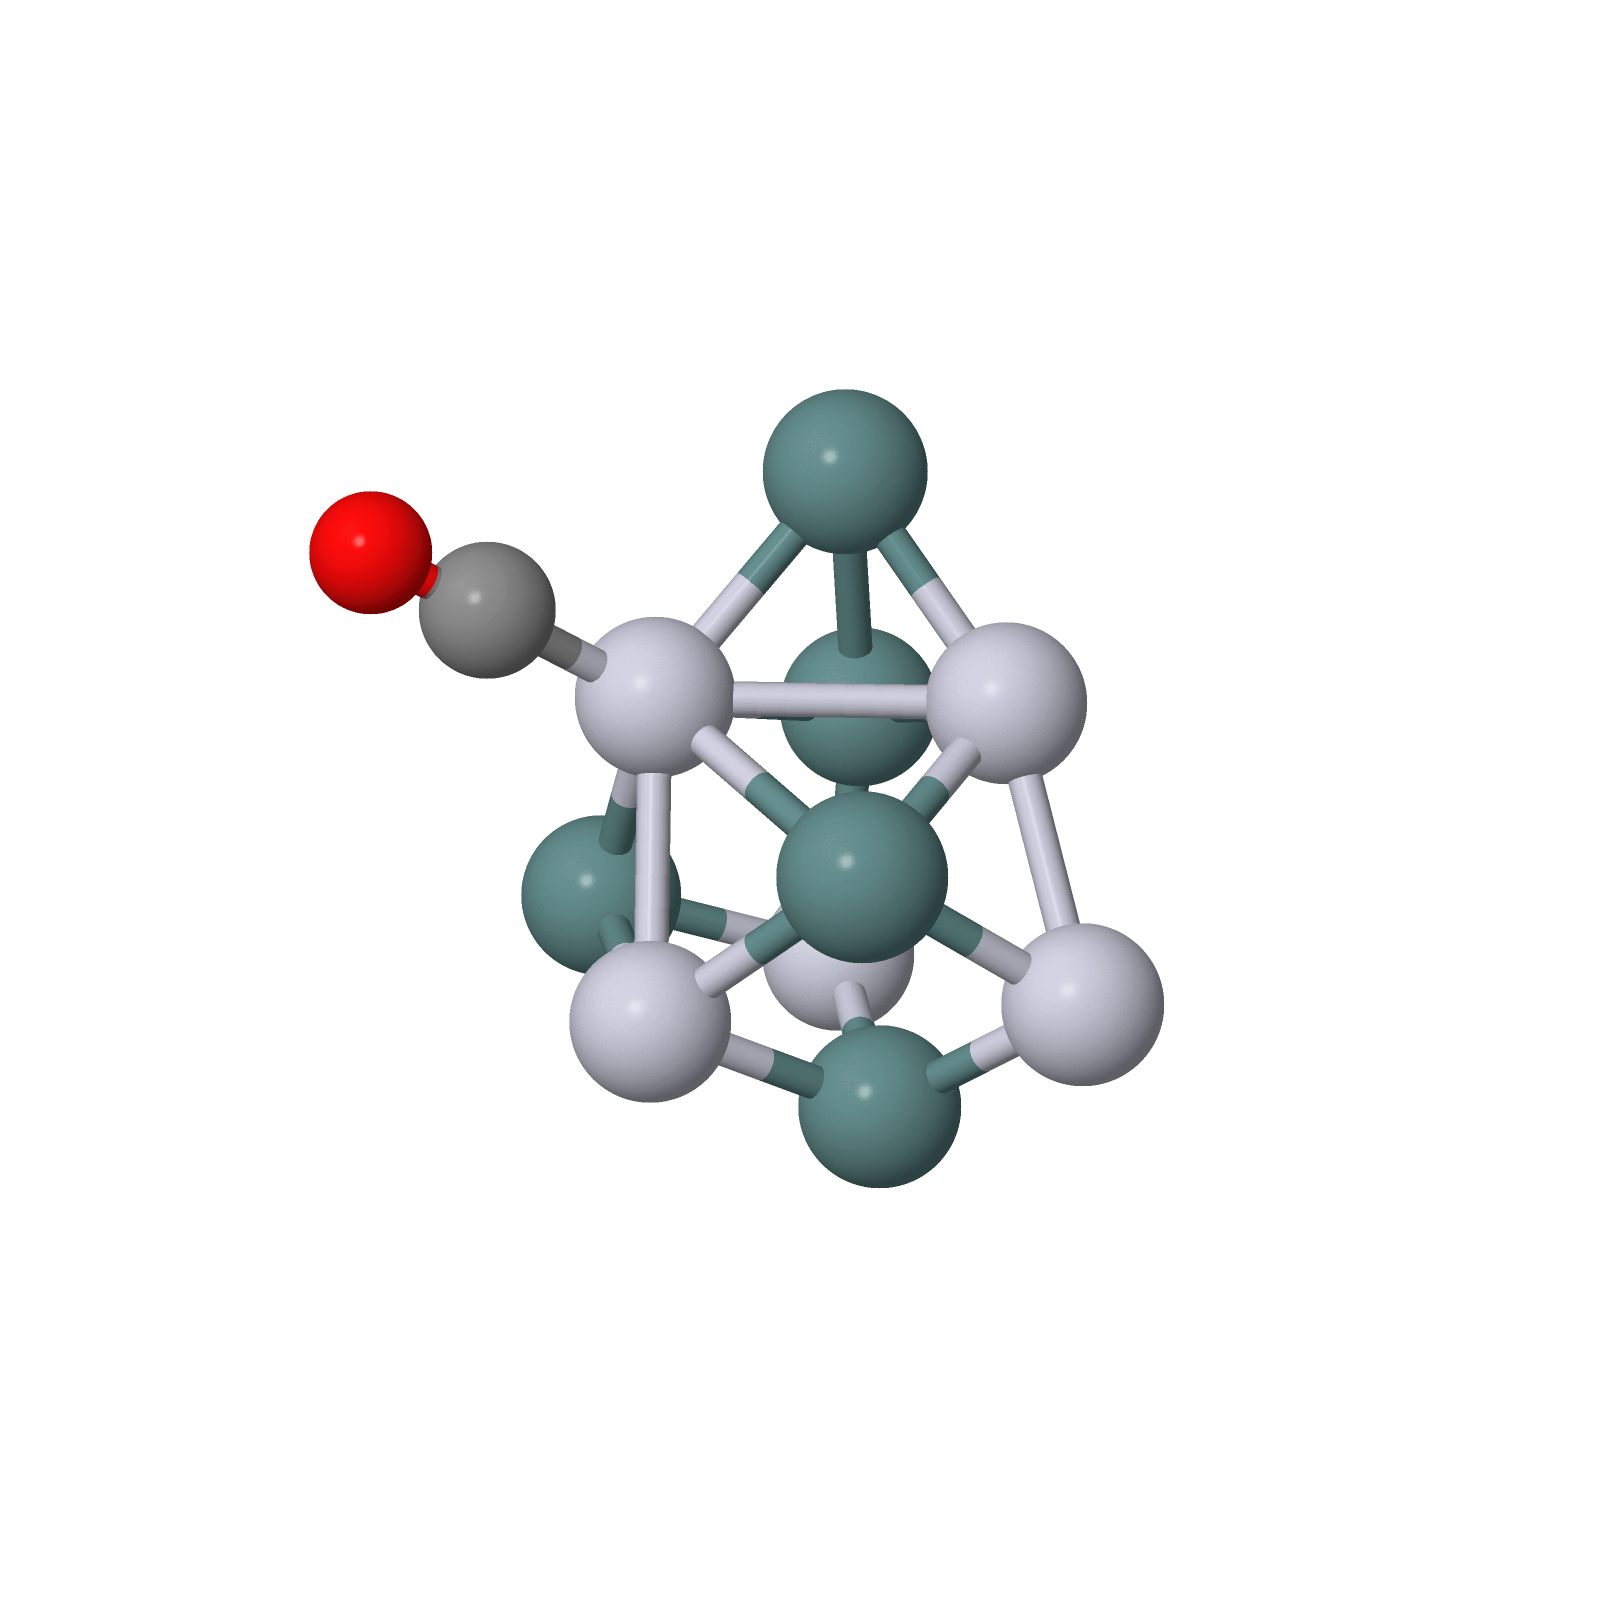
\includegraphics[width=\molw]{Pt5Ge5CO/pt5ge5_1_from_1xyz.png}};
\node[structure] (p5g5s2) at (\xmid,\rowtwo)
  {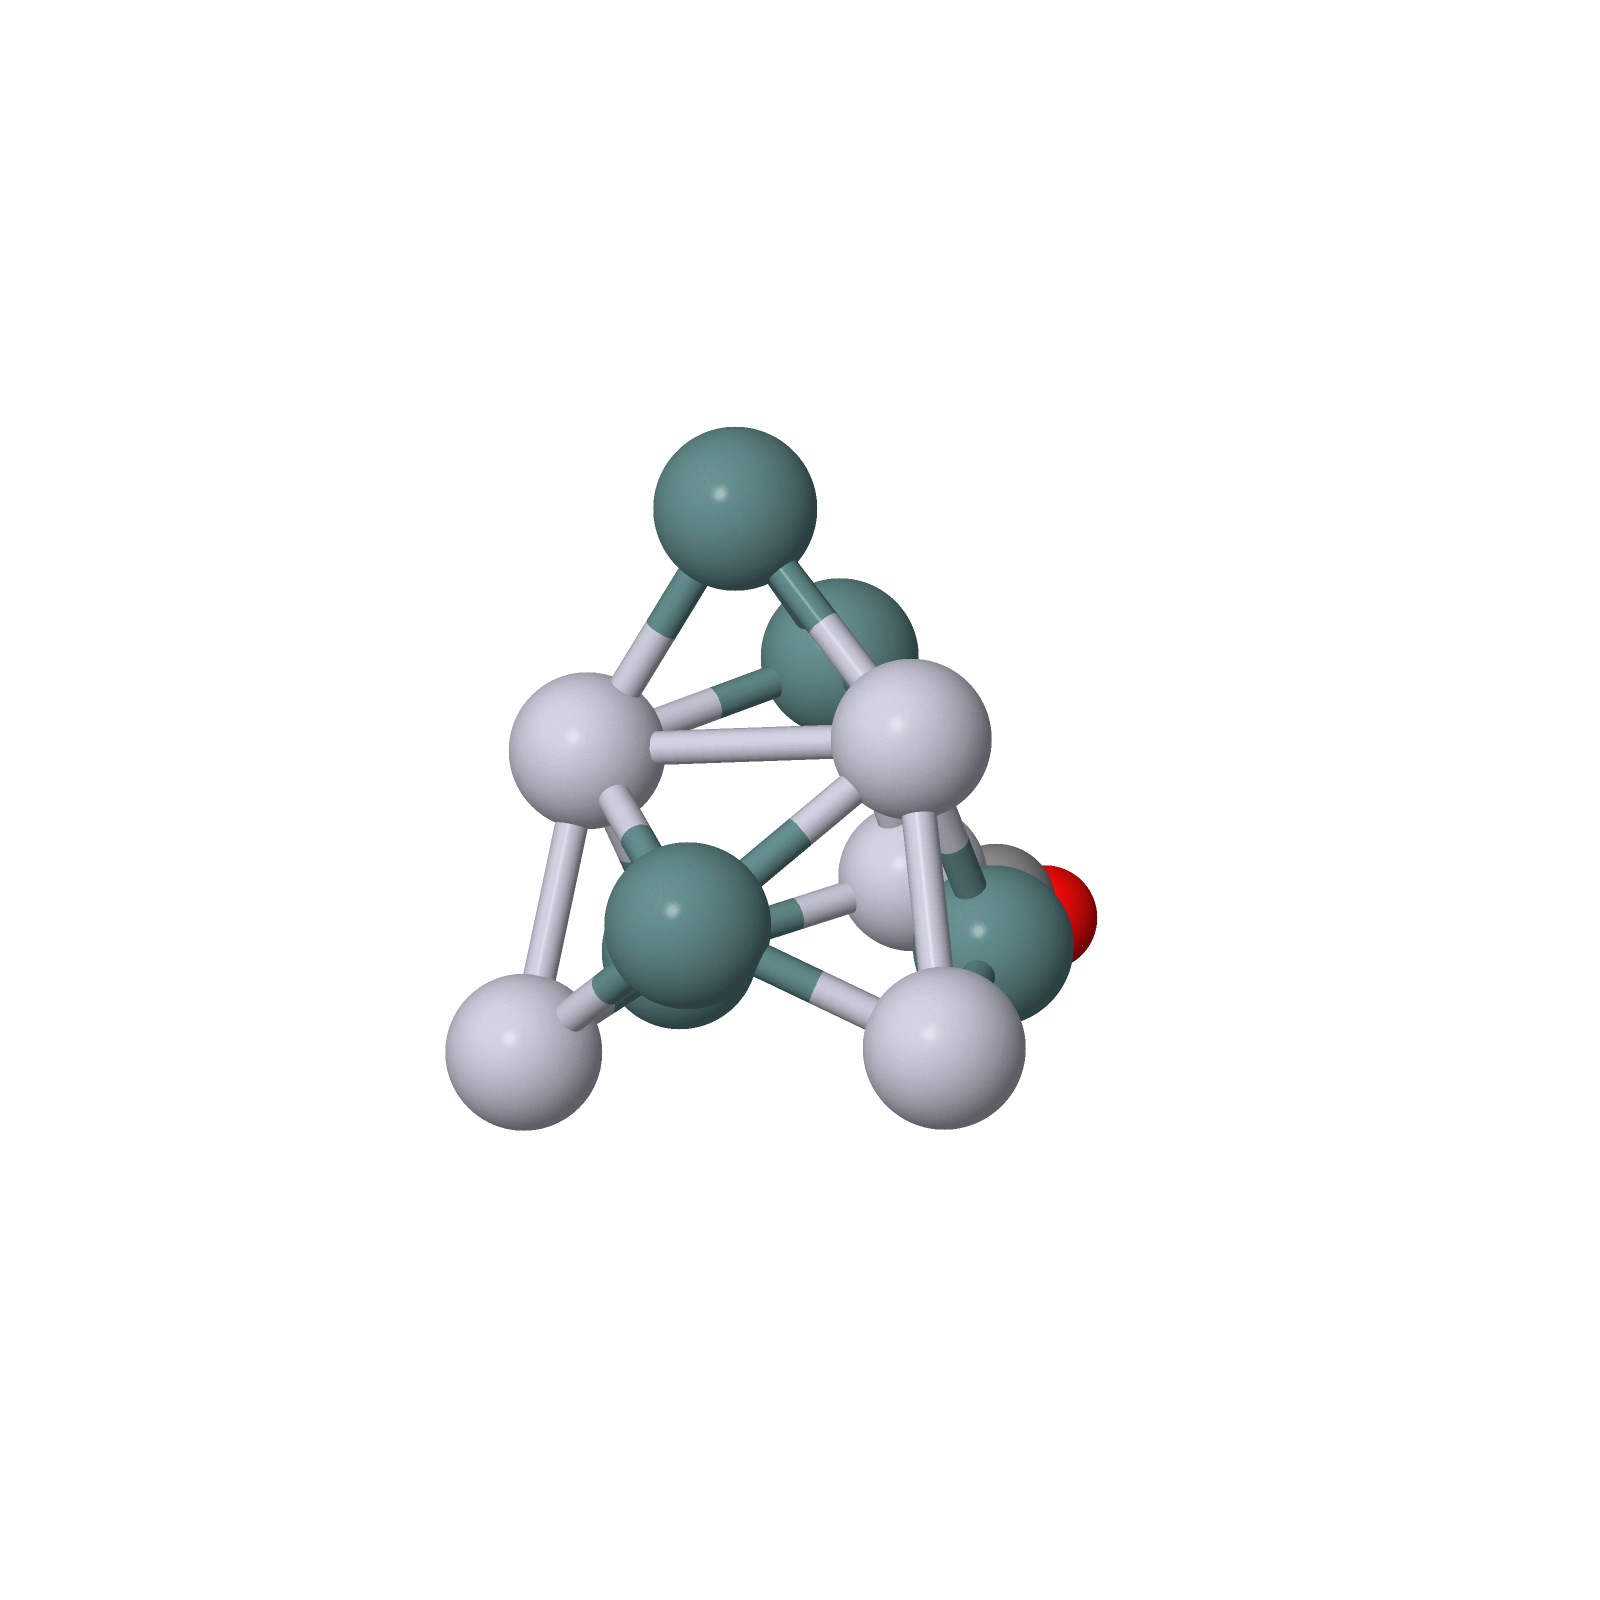
\includegraphics[width=\molw]{Pt5Ge5CO/Pt5Ge5_2_from_2xyzUnai.png}};
\node[structure] (p5g5s3) at (\xmidright,\rowtwo)
  {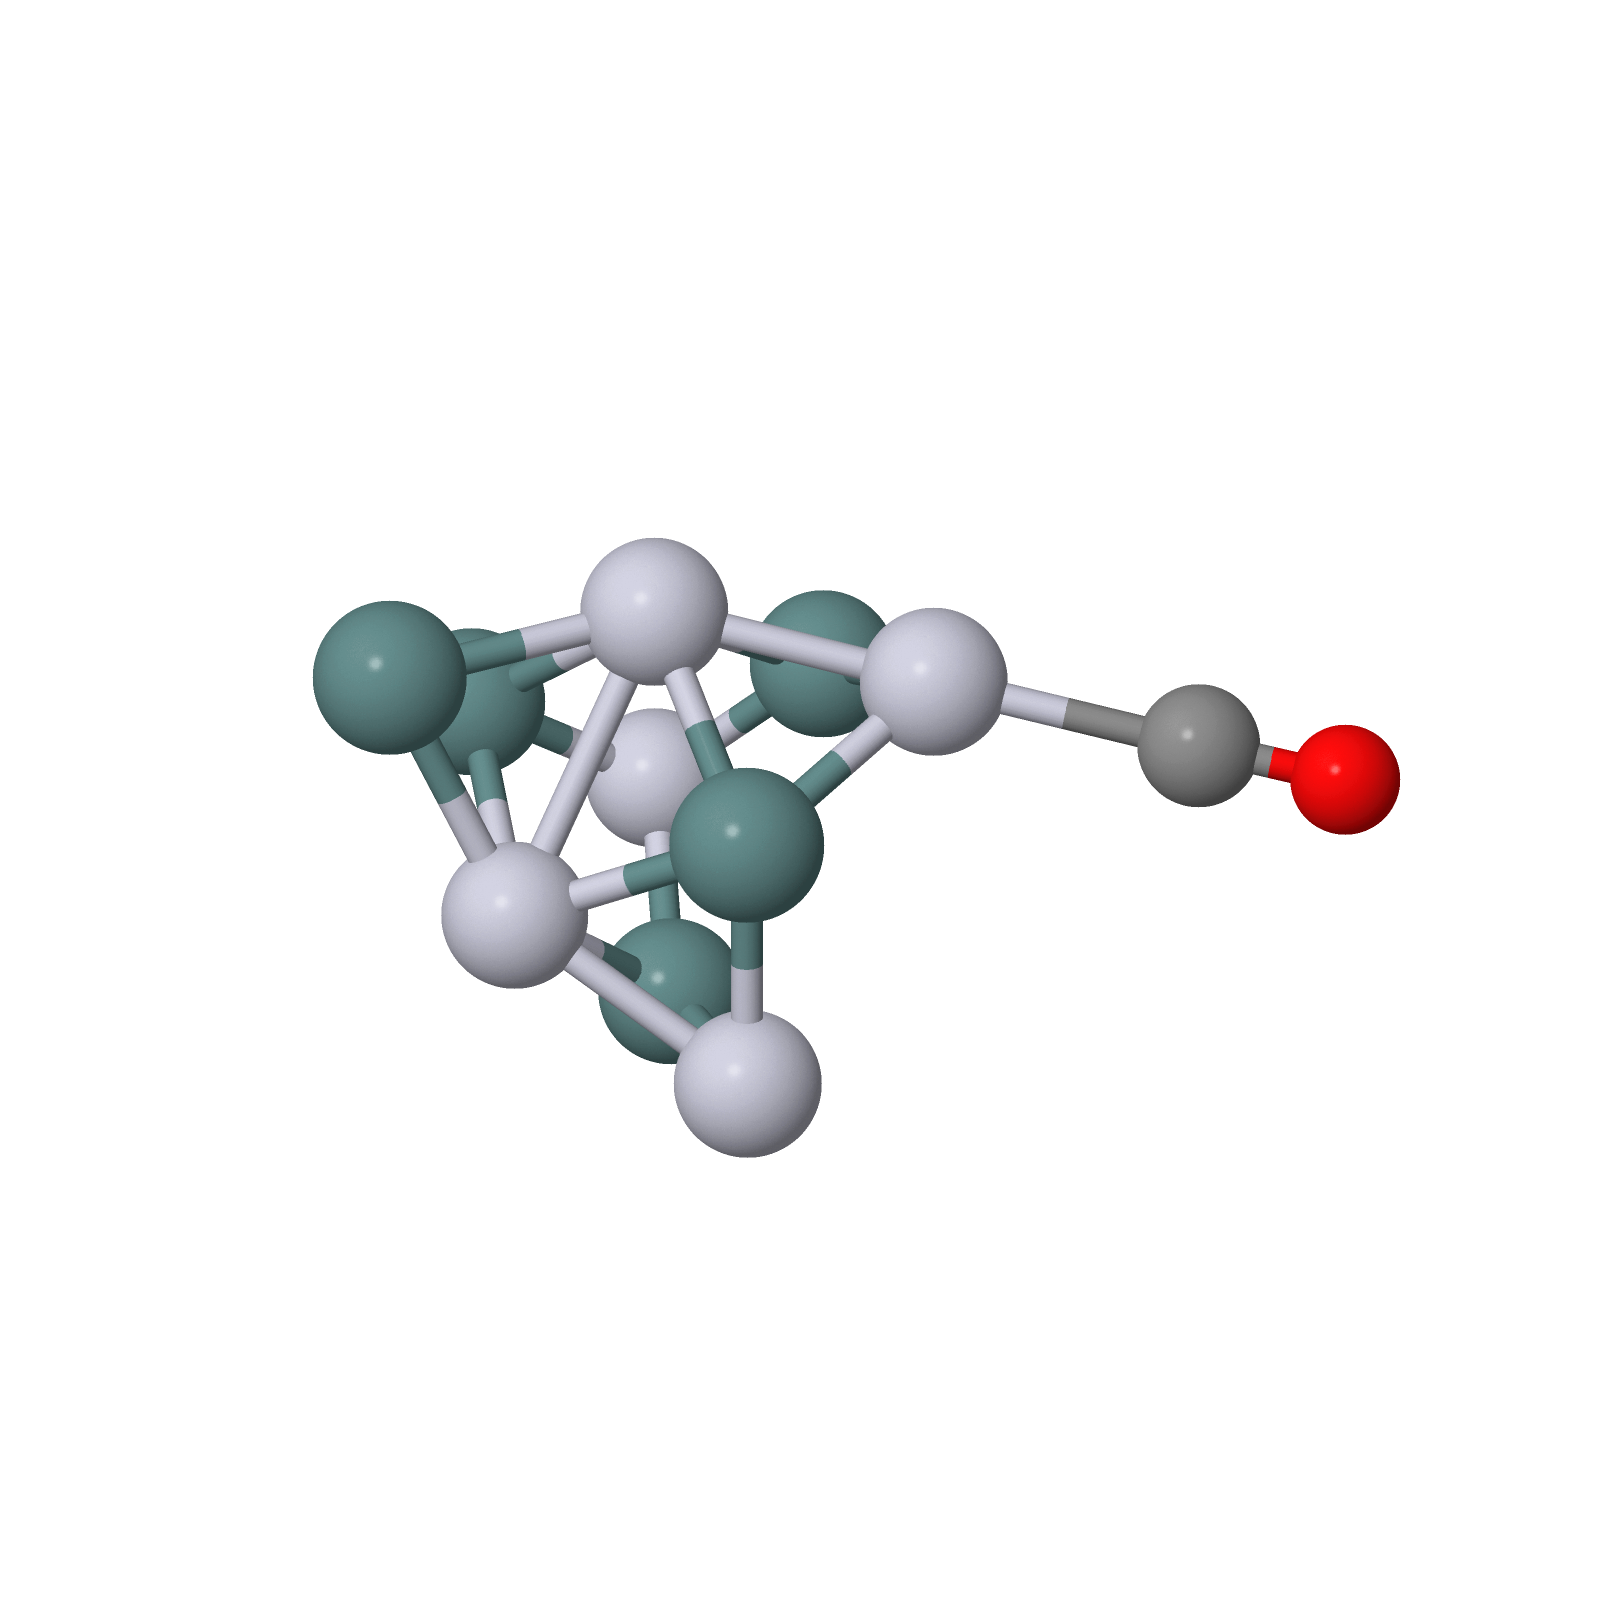
\includegraphics[width=\molw]{Pt5Ge5CO/Pt5Ge5_3_from_3xyzUnai.png}};

\node[rowlabel] at (0,{\rowtwo+1.48}) {\ce{Pt5Ge5CO}};
\node[sitelabel] at ([yshift=\labelshift]p5g5s1.center) {Sites 6/8};
\node[datalabel] at ([yshift=\datashift]p5g5s1.center) {$-2.076$ eV};
\node[sitelabel] at ([yshift=\labelshift]p5g5s2.center) {Sites 7/10};
\node[datalabel] at ([yshift=\datashift]p5g5s2.center) {$-1.661$ eV};
\node[sitelabel] at ([yshift=\labelshift]p5g5s3.center) {Site 4};
\node[datalabel] at ([yshift=\datashift]p5g5s3.center) {$-1.342$ eV};

% Pt4Ge6CO adsorption sites.
\node[structure] (p4g6s1) at (\xone,\rowthree)
  {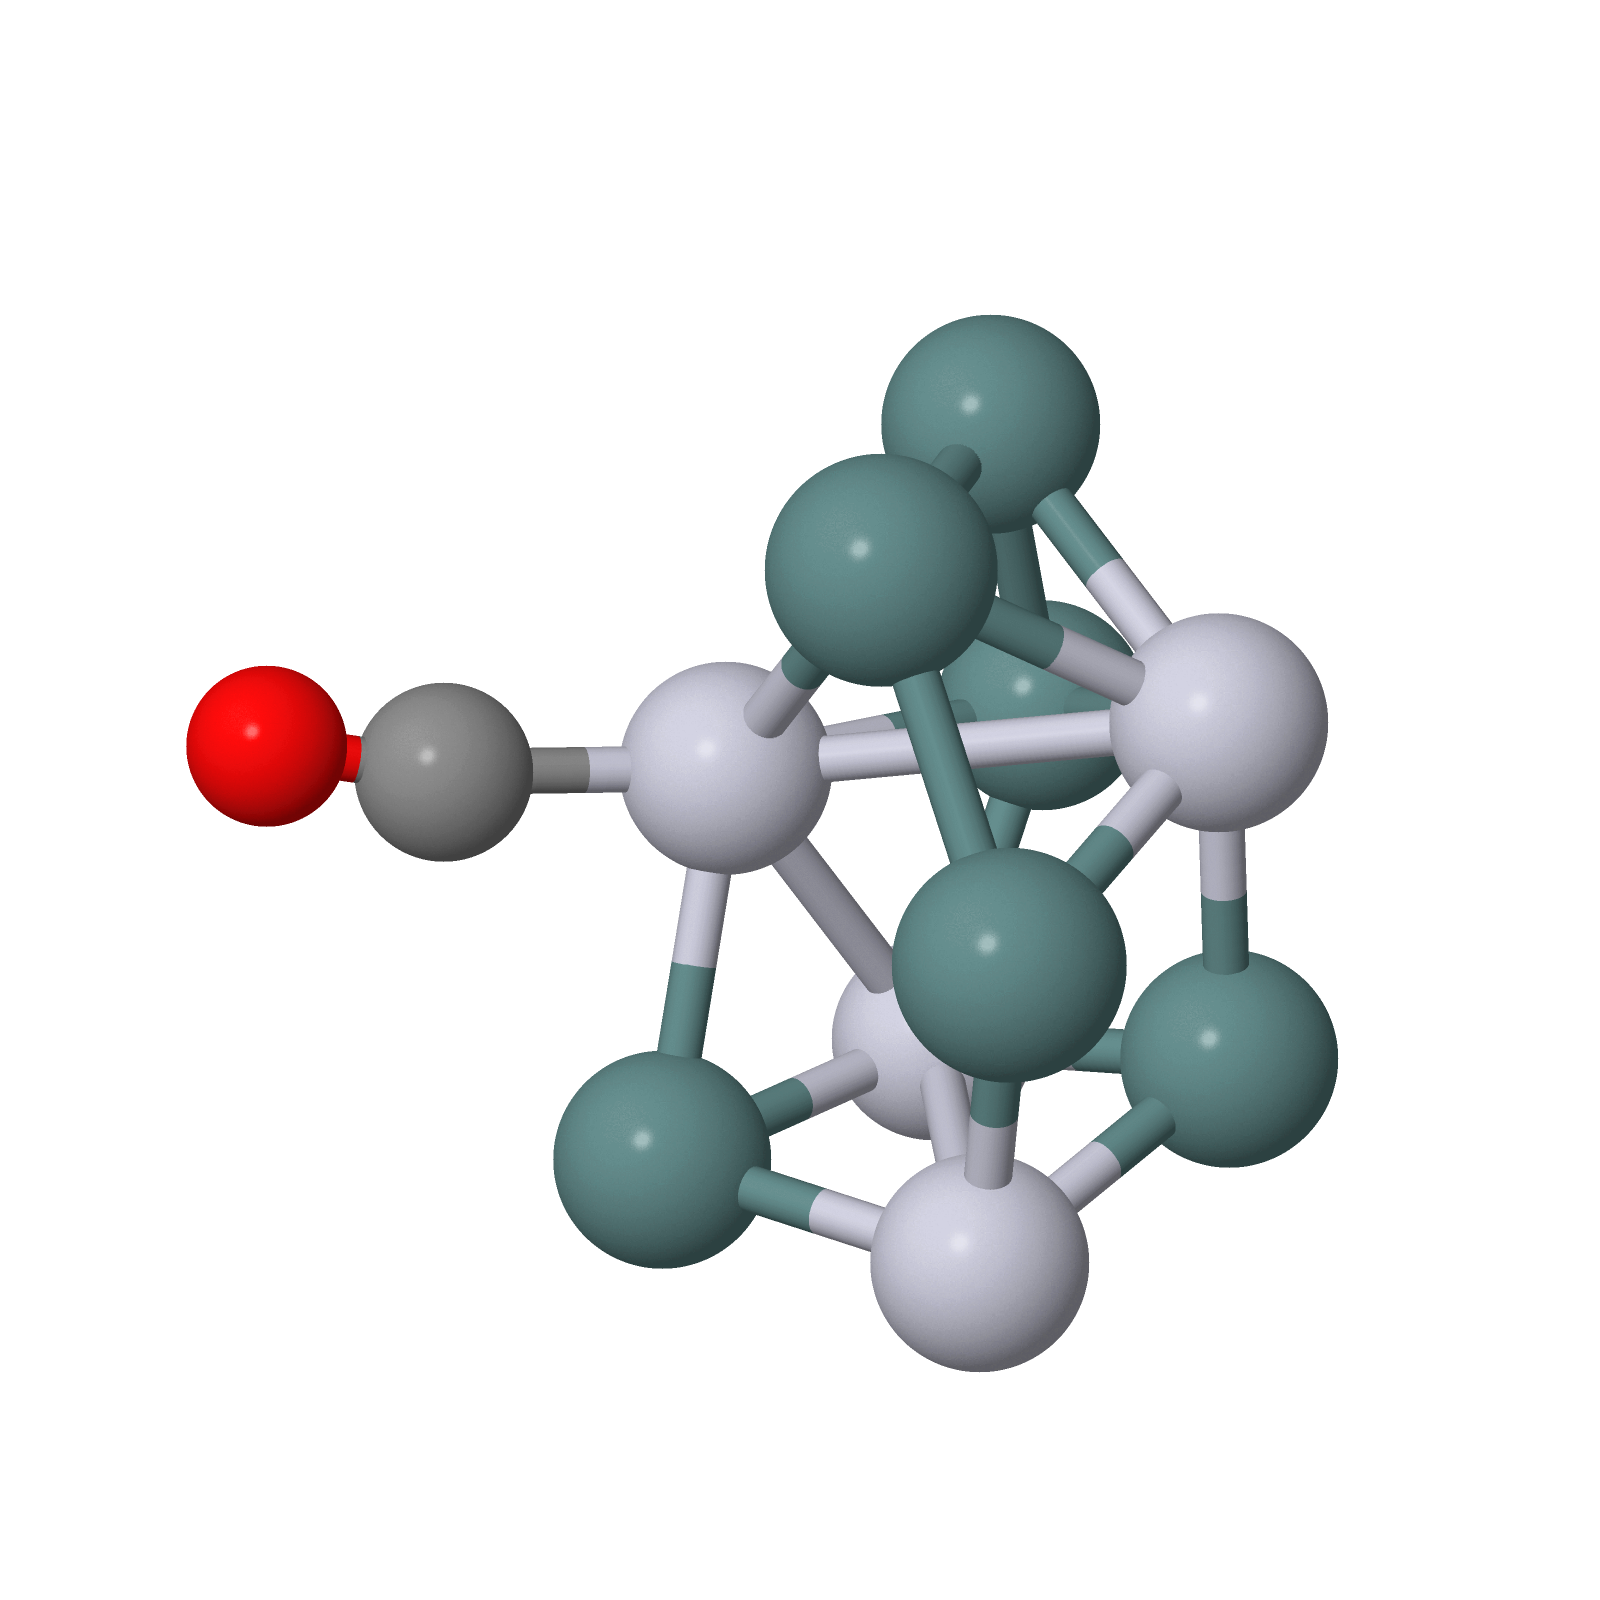
\includegraphics[width=\molwC]{pt4ge6_site01.png}};
\node[structure] (p4g6s2) at (\xtwo,\rowthree)
  {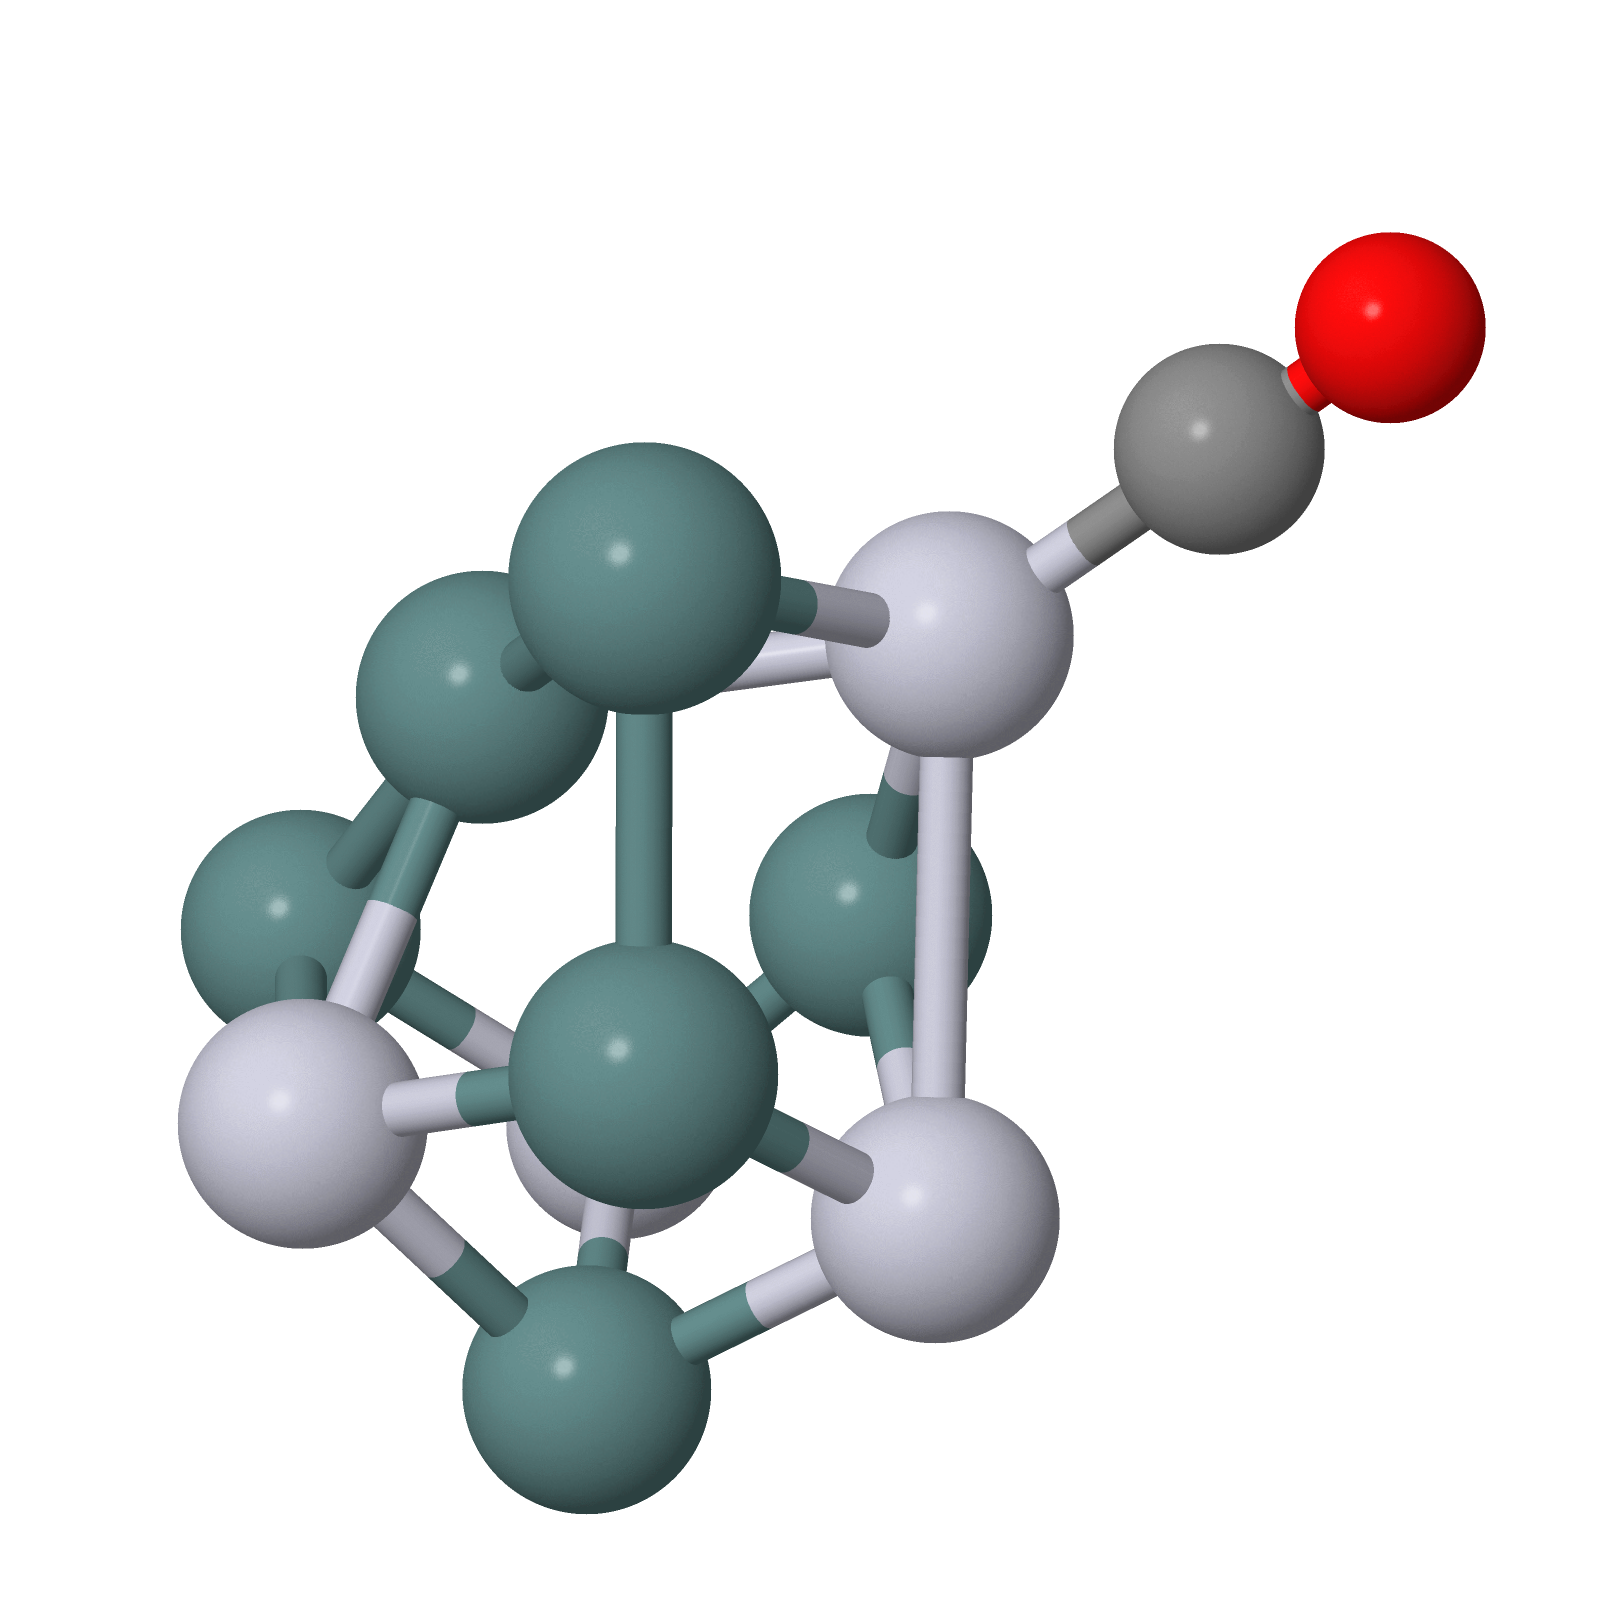
\includegraphics[width=\molwB]{pt4ge6_site02.png}};
\node[structure] (p4g6s5) at (\xthree,\rowthree)
  {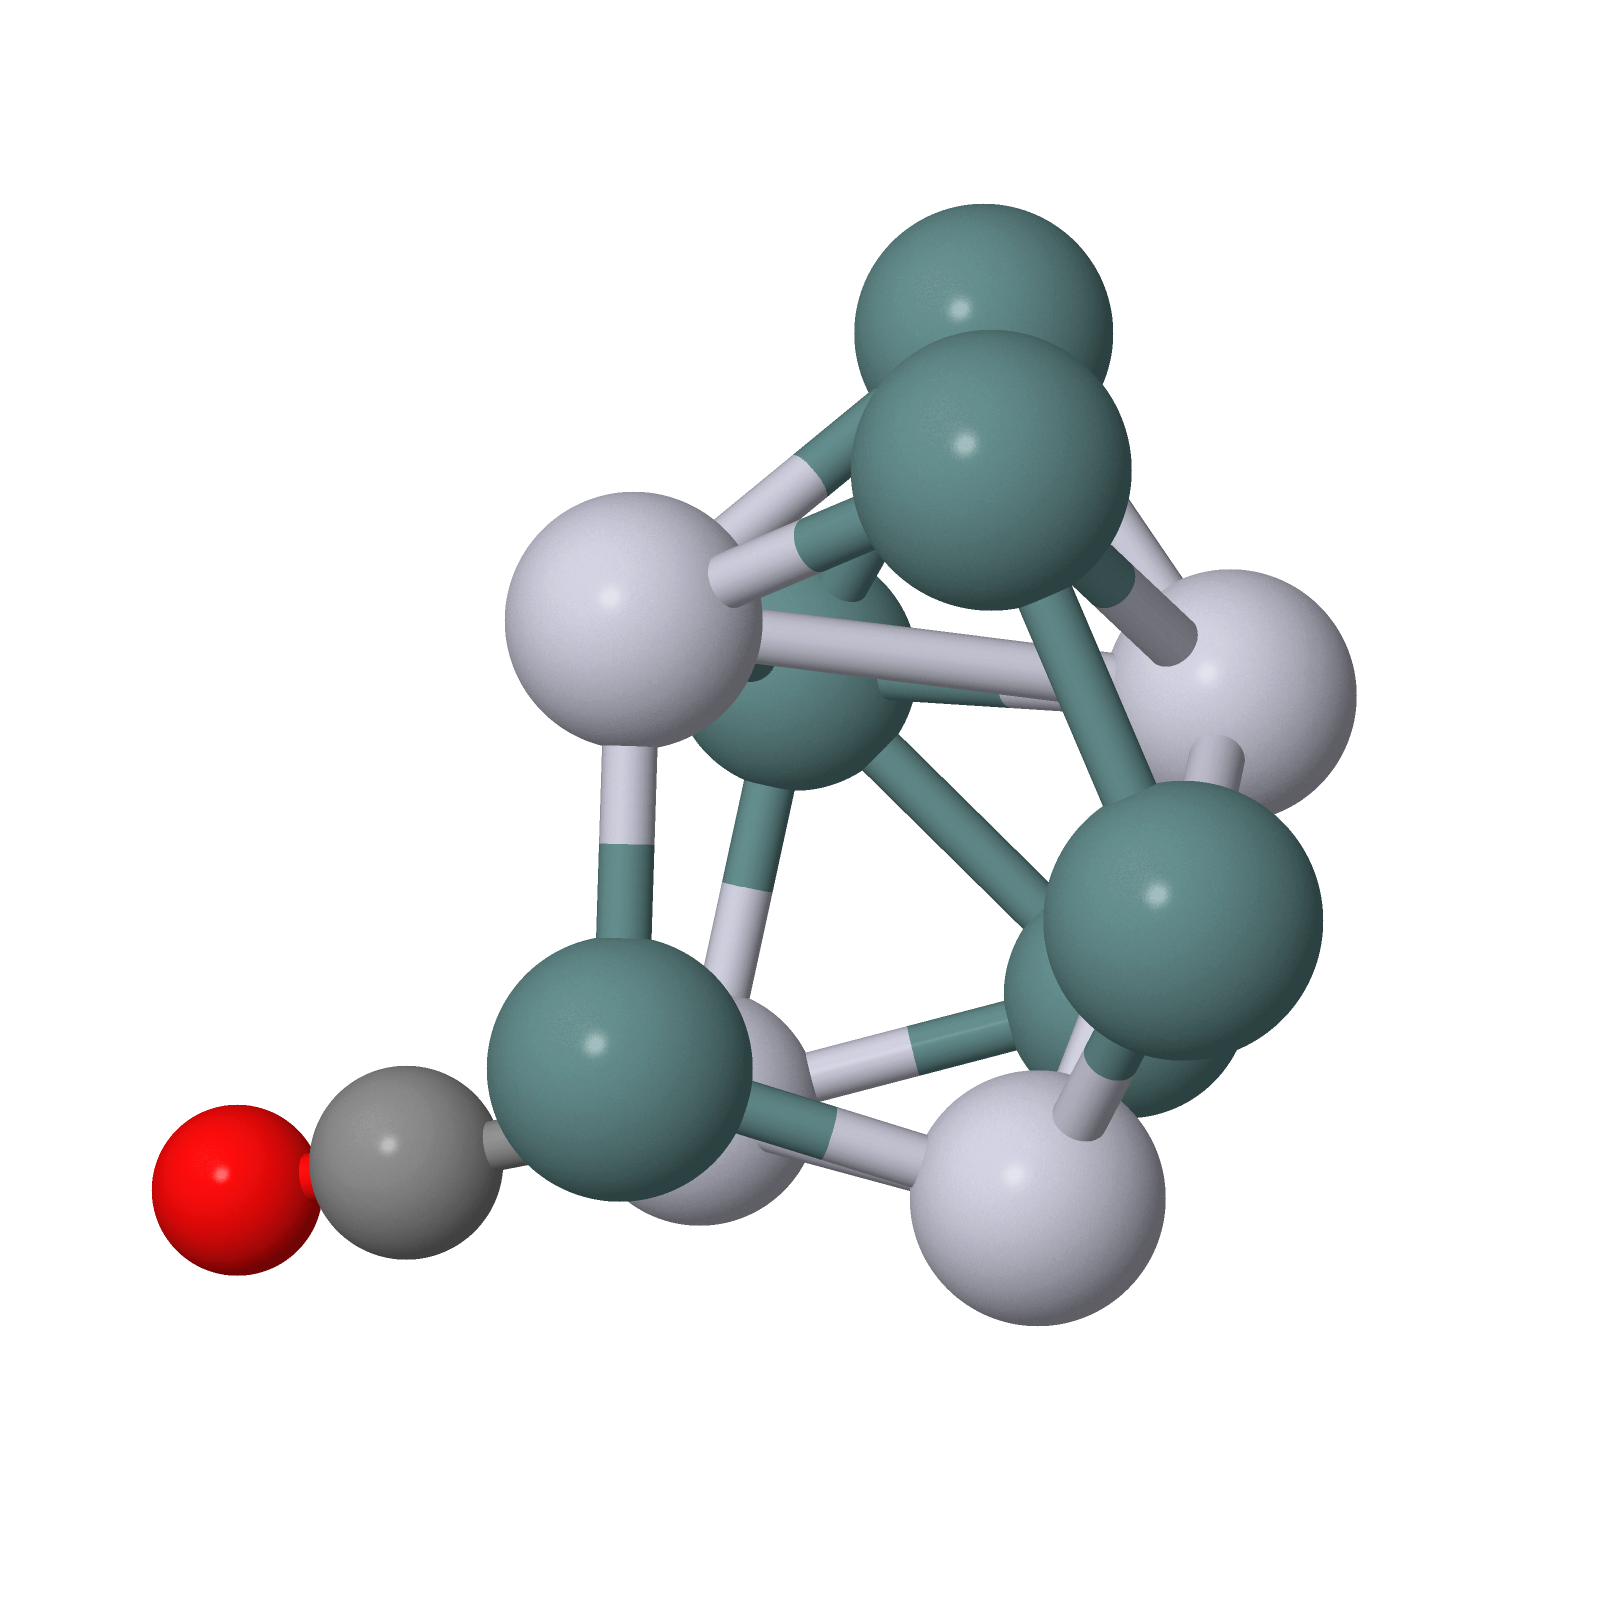
\includegraphics[width=\molwB]{pt4ge6_site05.png}};
\node[structure] (p4g6s7) at (\xfour,\rowthree)
  {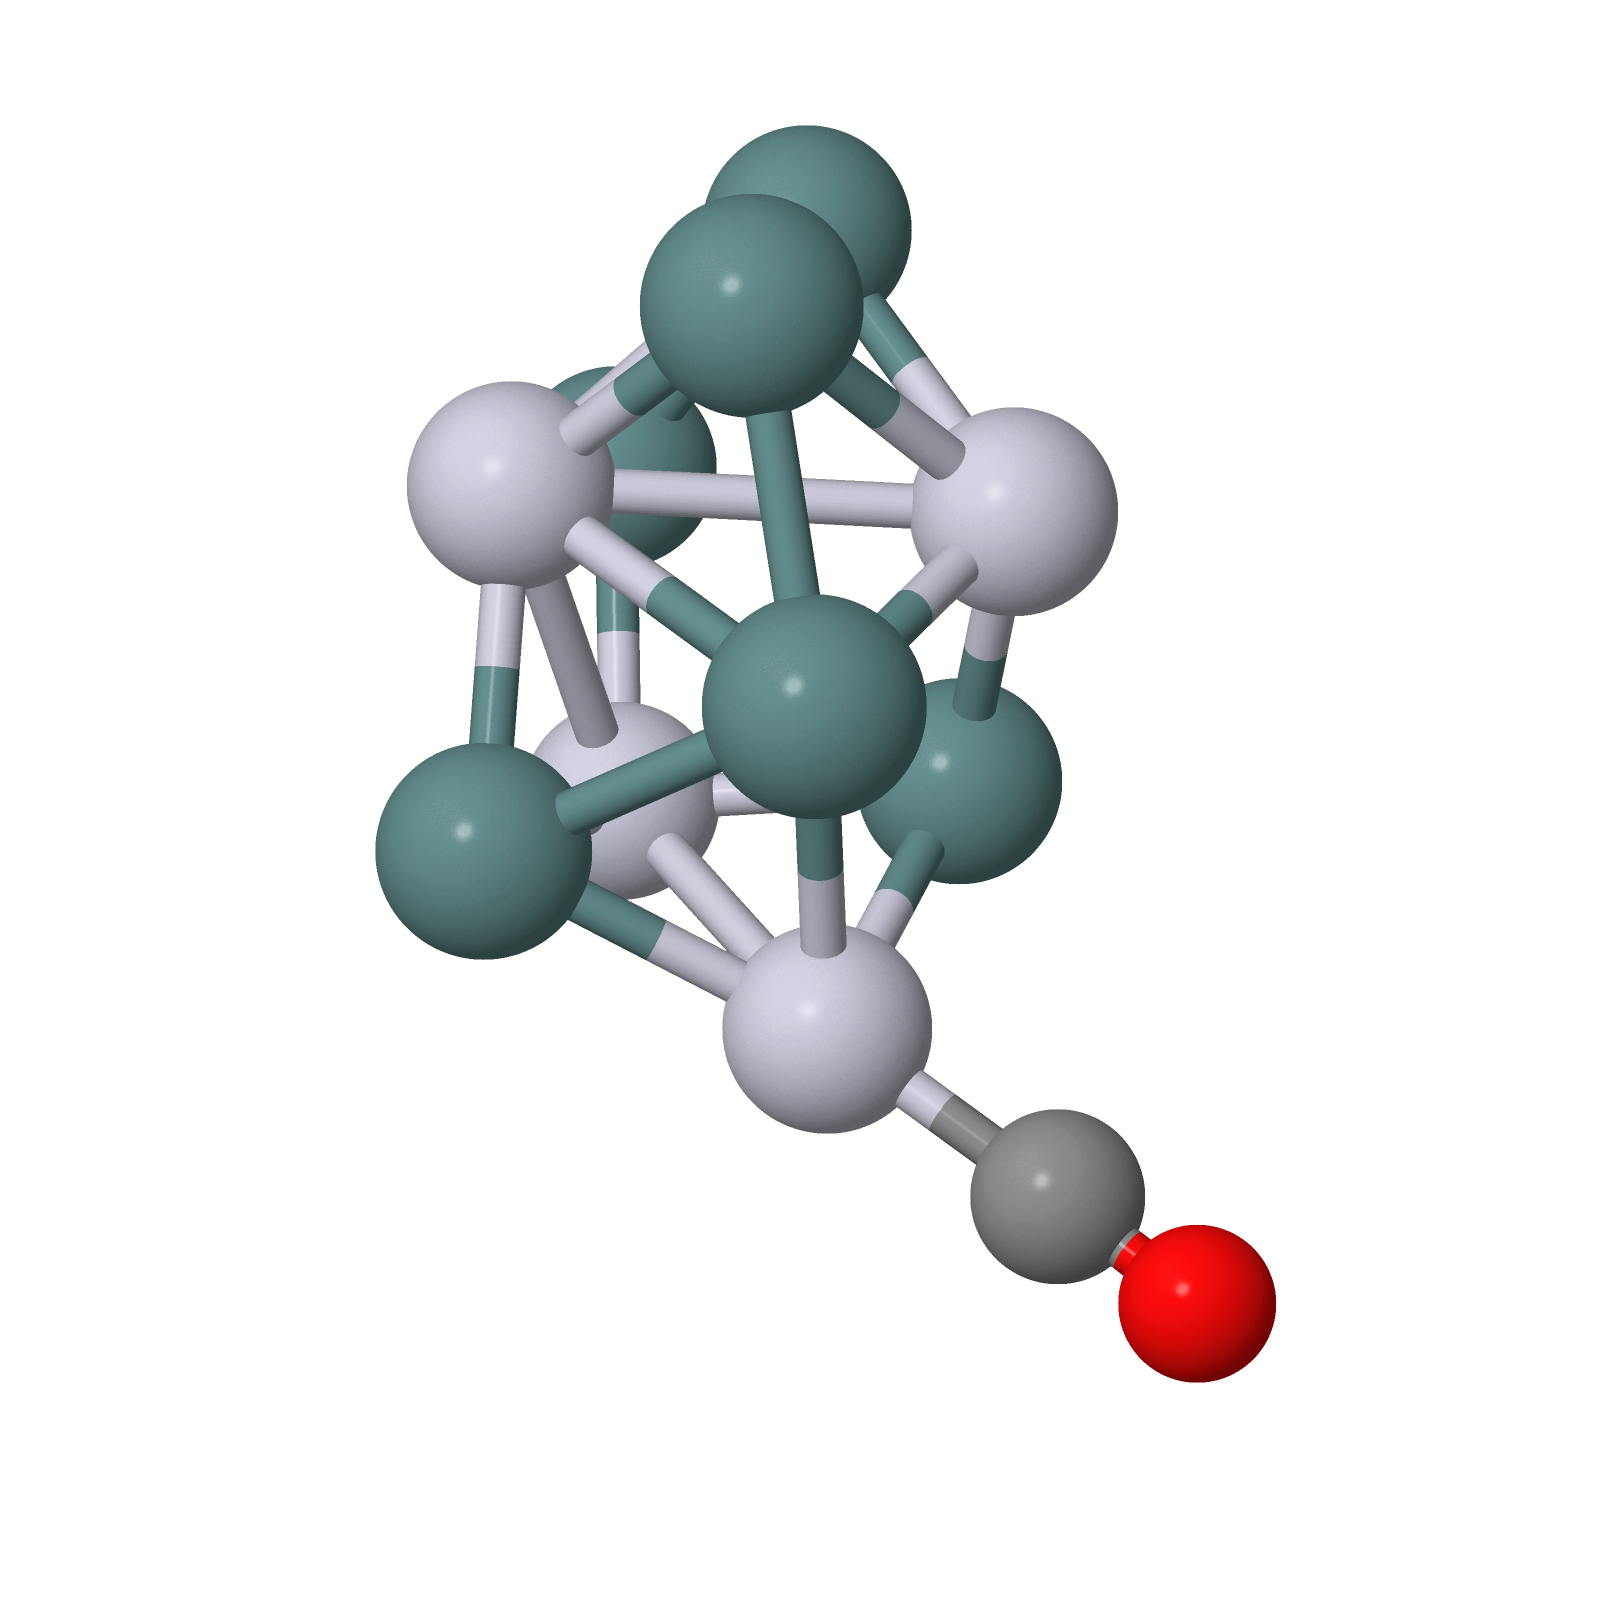
\includegraphics[width=\molwC]{pt4ge6_site07.png}};

\node[rowlabel] at (0,{\rowthree+1.48}) {\ce{Pt4Ge6CO}};
\node[sitelabel] at ([yshift=\labelshift]p4g6s1.center) {Site 1};
\node[datalabel] at ([yshift=\datashift]p4g6s1.center) {$-1.052$ eV};
\node[sitelabel] at ([yshift=\labelshift]p4g6s2.center) {Site 2};
\node[datalabel] at ([yshift=\datashift]p4g6s2.center) {$-1.305$ eV};
\node[sitelabel] at ([yshift=\labelshift]p4g6s5.center) {Site 5};
\node[datalabel] at ([yshift=\datashift]p4g6s5.center) {$-1.459$ eV};
\node[sitelabel] at ([yshift=\labelshift]p4g6s7.center) {Site 7};
\node[datalabel] at ([yshift=\datashift]p4g6s7.center) {$-1.458$ eV};

\end{tikzpicture}

\caption{Optimized carbonyl structures of the \ce{Pt6Ge4}, \ce{Pt5Ge5},
and \ce{Pt4Ge6} derivatives generated from the \ce{Pt10} parent framework
(top, middle, and bottom rows, respectively). Site labels retain the Pt atom
numbering of the parent structure shown in Figure~\ref{fig:tfg_site_numbering}.
For \ce{Pt6Ge4CO}, the four structures represent sites or site classes
$2$, $1/4$, $5/7$, and $9$ identified in the parent geometry. The paired
labels denote equivalent Pt positions represented by one optimized structure.
For \ce{Pt5Ge5CO}, three representative Pt positions are shown. The paired
positions 6/8 and 7/10 were considered equivalent and are represented by one
optimized structure each. For \ce{Pt4Ge6CO}, sites 5 and 7 converge to
effectively the same carbonyl minimum and are shown once as 5/7. The
corresponding $BE(\ce{CO})$ values are given
below each structure.}
\label{fig:tfg_ptgeco_series}
\end{figure}

% vim: set spell spelllang=en_us :

Table~\ref{tab:tfg_adsorption_descriptors} reports the crossed-parent and
GM-parent \ce{Pt10CO} results. Table~\ref{tab:tfg_bimetallic_adsorption_descriptors}
reports the binding, structural, and vibrational descriptors for the
crossed-parent \ce{Pt_xGe_{10-x}CO} series. The corresponding GM-parent Pt--Ge
data are given in Supporting
Table~\ref{tab:tfg_gm_bimetallic_adsorption_descriptors}.

\begin{table}[H]
\centering
\begin{singlespace}
\caption{Relative energies, \ce{CO} binding energies, and structural and
vibrational descriptors for the distinct \ce{Pt10CO} minima obtained from the
\ce{Pt5Ge5}-derived and global-minimum parent structures. Within each parent
geometry and multiplicity series, $\Delta E_0$ is measured relative to the
lowest carbonyl minimum in that series. Each $BE$ uses free singlet \ce{CO}
and the optimized bare \ce{Pt10} cluster with the same parent framework and
multiplicity as the corresponding carbonyl. Site labels identify the initial
Pt placements; labels separated by ``/'' denote placements that converge to
the same optimized minimum.}
\label{tab:tfg_adsorption_descriptors}
\renewcommand{\arraystretch}{0.92}
\begin{tabular}{cclcccc}
\toprule
{$\Delta E_0$ / eV} & {$2S+1$} & {Site} & {$BE$ / eV} &
{$r(\ce{Pt-C})$ / \si{\angstromunit}} & {$r(\ce{C-O})$ / \si{\angstromunit}} &
{$\nu(\ce{CO})$ / \si{\per\centi\metre}} \\
\midrule
\multicolumn{7}{l}{\textit{\ce{Pt5Ge5}-derived crossed-parent series}} \\
\multicolumn{7}{l}{\quad $2S+1=3$} \\
0.000 & 3 & 6    & -2.657 & 1.831 & 1.158 & 2020.0 \\
0.007 & 3 & 8/10 & -2.650 & 1.831 & 1.159 & 2012.4 \\
0.068 & 3 & 3/5  & -2.590 & 1.835 & 1.159 & 2014.3 \\
0.079 & 3 & 4    & -2.579 & 1.836 & 1.159 & 2013.0 \\
0.164 & 3 & 2    & -2.493 & 1.833 & 1.160 & 2005.9 \\
0.165 & 3 & 7    & -2.493 & 1.836 & 1.159 & 2016.0 \\
0.502 & 3 & 1/9  & -2.156 & 1.837 & 1.156 & 2033.7 \\
\multicolumn{7}{l}{\quad $2S+1=5$} \\
0.000 & 5 & 5/7  & -2.645 & 1.834 & 1.159 & 2012.5 \\
0.334 & 5 & 2/10 & -2.311 & 1.834 & 1.158 & 2017.1 \\
0.421 & 5 & 3/6  & -2.223 & 1.834 & 1.156 & 2032.6 \\
0.456 & 5 & 1/8  & -2.189 & 1.841 & 1.159 & 2011.0 \\
0.635 & 5 & 4/9  & -2.010 & 1.835 & 1.159 & 2006.3 \\
\midrule
\multicolumn{7}{l}{\textit{GM-parent series}} \\
\multicolumn{7}{l}{\quad $2S+1=5$} \\
0.000 & 5 & 3/6/9 & -2.275 & 1.820 & 1.158 & 2021.3 \\
0.049 & 5 & 1/2/8 & -2.226 & 1.819 & 1.159 & 2020.6 \\
0.670 & 5 & 7/10 & -1.605 & 1.876 & 1.155 & 2014.3 \\
0.709 & 5 & 5 & -1.566 & 1.876 & 1.156 & 2012.5 \\
0.728 & 5 & 4 & -1.547 & 1.877 & 1.156 & 2012.2 \\
\multicolumn{7}{l}{\quad $2S+1=7$} \\
0.000 & 7 & 8/9 & -2.353 & 1.820 & 1.159 & 2018.9 \\
0.000 & 7 & 1/2/3/6 & -2.353 & 1.820 & 1.159 & 2018.9 \\
0.598 & 7 & 4/5/7/10 & -1.755 & 1.877 & 1.155 & 2013.2 \\
\multicolumn{7}{l}{\quad $2S+1=9$} \\
0.000 & 9 & 1/2/3/6/8/9 & -1.595 & 1.857 & 1.156 & 2018.0 \\
0.015 & 9 & 4/5/7/10 & -1.580 & 1.888 & 1.155 & 2014.7 \\
\midrule
--- & 1 & free \ce{CO} & --- & --- & 1.137 & 2129.0 \\
\bottomrule
\end{tabular}
\end{singlespace}
\end{table}

\begin{table}[H]
\centering
\begin{singlespace}
\caption{\ce{CO} binding energies at the sampled Pt sites, together with
structural and vibrational descriptors, for the Ge-containing carbonyls
obtained from the crossed-parent models derived from the original \ce{Pt10}
framework. Rows are ordered by $BE$ within each composition. All carbonyls in
this table are singlets. Each $BE$ uses free singlet \ce{CO} and the isolated
bare crossed-parent cluster of the corresponding composition as references.
The corresponding global-minimum-parent data are reported separately in
Supporting Table~\ref{tab:tfg_gm_bimetallic_adsorption_descriptors}. Site
labels identify the initial Pt placements. Grouped labels denote positions
represented by the same optimized result, either because they are equivalent
in the parent structure or because they converge to the same minimum.}
\label{tab:tfg_bimetallic_adsorption_descriptors}
\renewcommand{\arraystretch}{0.92}
\begin{tabular}{lccccc}
\toprule
{Composition} &  {Site} & {$BE$ / eV} &
{$r(\ce{Pt-C})$ / \si{\angstromunit}} & {$r(\ce{C-O})$ / \si{\angstromunit}} &
{$\nu(\ce{CO})$ / \si{\per\centi\metre}} \\
\midrule
\ce{Pt6Ge4CO}  & 2    & -2.246 & 1.841 & 1.158 & 2019.21 \\
\ce{Pt6Ge4CO}  & 9    & -2.245 & 1.870 & 1.153 & 2037.50 \\
\ce{Pt6Ge4CO}  & 1/4  & -2.235 & 1.838 & 1.159 & 2018.43 \\
\ce{Pt6Ge4CO}  & 5/7    & -1.567 & 1.903 & 1.154 & 2018.58 \\
\midrule
\ce{Pt5Ge5CO}  & 6/8  & -2.076 & 1.895 & 1.157 & 2003.10 \\
\ce{Pt5Ge5CO}  & 7/10 & -1.661 & 1.888 & 1.154 & 2027.46 \\
\ce{Pt5Ge5CO}  & 4  & -1.342 & 1.924 & 1.156 & 2004.80 \\
\midrule
\ce{Pt4Ge6CO}  & 5/7 & -1.459 & 1.896 & 1.155 & 2019.36 \\
\ce{Pt4Ge6CO}  & 2 & -1.305 & 1.882 & 1.155 & 2020.88 \\
\ce{Pt4Ge6CO}  & 1 & -1.052 & 1.875 & 1.158 & 2004.13 \\
\bottomrule
\end{tabular}
\\
\end{singlespace}
\end{table}

Figure~\ref{fig:tfg_adsorption_distribution} summarizes the binding-energy
ranges and the mean values calculated from the data in the tables.

\begin{figure}[H]
\centering
\definecolor{ptten}{RGB}{35,35,35}
\definecolor{crossedparent}{RGB}{35,35,35}
\definecolor{globalparent}{RGB}{0,90,190}

\begin{tikzpicture}
\begin{axis}[
  width=0.76\linewidth,
  height=5.4cm,
  xmin=0.45, xmax=3.55,
  ymin=-2.85, ymax=-0.25,
  xtick={0.95,2.00,2.65,3.25},
  xticklabels={\ce{Pt10CO},\ce{Pt6Ge4CO},\ce{Pt5Ge5CO},\ce{Pt4Ge6CO}},
  ylabel={$BE(\ce{CO})$ / eV},
  ylabel style={yshift=-2pt},
  tick label style={font=\small},
  label style={font=\small},
  grid=major,
  grid style={gray!20},
  axis line style={black!70},
  legend style={
    at={(1.02,0.98)},
    anchor=north west,
    draw=none,
    inner sep=2pt,
    row sep=1pt,
    font=\scriptsize,
    legend columns=1
  }
]
\addlegendimage{only marks,mark=*,mark size=2.5pt,black}
\addlegendentry{Singlet}
\addlegendimage{only marks,mark=square*,mark size=2.5pt,black}
\addlegendentry{Triplet}
\addlegendimage{only marks,mark=triangle*,mark size=2.8pt,black}
\addlegendentry{Quintet}
\addlegendimage{only marks,mark=pentagon*,mark size=3.0pt,black}
\addlegendentry{Septet}
\addlegendimage{only marks,mark=diamond*,mark size=2.8pt,black}
\addlegendentry{Nonet}
% Each vertical bar shows the minimum--maximum interval and each marker the
% mean over all Pt sites represented by the corresponding series. Horizontal
% offsets are used only for readability.
% Crossed-parent Pt10: triplet and quintet.
\addplot[ptten,line width=1.0pt] coordinates {(0.56,-2.657) (0.56,-2.156)};
\addplot[ptten,line width=1.0pt] coordinates {(0.50,-2.657) (0.62,-2.657)};
\addplot[ptten,line width=1.0pt] coordinates {(0.50,-2.156) (0.62,-2.156)};
\addplot[only marks,mark=square*,mark size=3.0pt,ptten] coordinates {(0.56,-2.501)};
\addplot[ptten,line width=1.0pt] coordinates {(0.74,-2.645) (0.74,-2.010)};
\addplot[ptten,line width=1.0pt] coordinates {(0.68,-2.645) (0.80,-2.645)};
\addplot[ptten,line width=1.0pt] coordinates {(0.68,-2.010) (0.80,-2.010)};
\addplot[only marks,mark=triangle*,mark size=3.0pt,ptten] coordinates {(0.74,-2.276)};
% Original Pt10 global-minimum parent: nonet, septet, and quintet.
\addplot[globalparent,densely dashed,line width=1.0pt] coordinates {(0.96,-1.595) (0.96,-1.580)};
\addplot[globalparent,densely dashed,line width=1.0pt] coordinates {(0.90,-1.595) (1.02,-1.595)};
\addplot[globalparent,densely dashed,line width=1.0pt] coordinates {(0.90,-1.580) (1.02,-1.580)};
\addplot[only marks,mark=diamond*,mark size=3.0pt,globalparent,
  mark options={fill=white,draw=globalparent,line width=0.8pt}] coordinates {(0.96,-1.588)};
\addplot[globalparent,densely dashed,line width=1.0pt] coordinates {(1.18,-2.353) (1.18,-1.755)};
\addplot[globalparent,densely dashed,line width=1.0pt] coordinates {(1.12,-2.353) (1.24,-2.353)};
\addplot[globalparent,densely dashed,line width=1.0pt] coordinates {(1.12,-1.755) (1.24,-1.755)};
\addplot[only marks,mark=pentagon*,mark size=3.2pt,globalparent,
  mark options={fill=white,draw=globalparent,line width=0.8pt}] coordinates {(1.18,-2.114)};
\addplot[globalparent,densely dashed,line width=1.0pt] coordinates {(1.40,-2.275) (1.40,-1.547)};
\addplot[globalparent,densely dashed,line width=1.0pt] coordinates {(1.34,-2.275) (1.46,-2.275)};
\addplot[globalparent,densely dashed,line width=1.0pt] coordinates {(1.34,-1.547) (1.46,-1.547)};
\addplot[only marks,mark=triangle*,mark size=3.0pt,globalparent,
  mark options={fill=white,draw=globalparent,line width=0.8pt}] coordinates {(1.40,-1.982)};
% Pt6Ge4: crossed-parent singlet and GM-parent triplet.
\addplot[crossedparent,line width=1.0pt] coordinates {(1.80,-2.246) (1.80,-1.567)};
\addplot[crossedparent,line width=1.0pt] coordinates {(1.74,-2.246) (1.86,-2.246)};
\addplot[crossedparent,line width=1.0pt] coordinates {(1.74,-1.567) (1.86,-1.567)};
\addplot[only marks,mark=*,mark size=3.2pt,crossedparent] coordinates {(1.80,-2.016)};
\addplot[globalparent,densely dashed,line width=1.0pt] coordinates {(2.00,-1.947) (2.00,-1.207)};
\addplot[globalparent,densely dashed,line width=1.0pt] coordinates {(1.94,-1.947) (2.06,-1.947)};
\addplot[globalparent,densely dashed,line width=1.0pt] coordinates {(1.94,-1.207) (2.06,-1.207)};
\addplot[
  only marks,mark=square*,mark size=3.0pt,globalparent,
  mark options={fill=white,draw=globalparent,line width=0.8pt}
] coordinates {(2.00,-1.600)};
% Pt5Ge5: crossed parent and GM parent.
\addplot[crossedparent,line width=1.0pt] coordinates {(2.55,-2.076) (2.55,-1.342)};
\addplot[crossedparent,line width=1.0pt] coordinates {(2.49,-2.076) (2.61,-2.076)};
\addplot[crossedparent,line width=1.0pt] coordinates {(2.49,-1.342) (2.61,-1.342)};
\addplot[only marks,mark=*,mark size=3.0pt,crossedparent] coordinates {(2.55,-1.763)};
\addplot[globalparent,densely dashed,line width=1.0pt] coordinates {(2.75,-1.346) (2.75,-0.788)};
\addplot[globalparent,densely dashed,line width=1.0pt] coordinates {(2.69,-1.346) (2.81,-1.346)};
\addplot[globalparent,densely dashed,line width=1.0pt] coordinates {(2.69,-0.788) (2.81,-0.788)};
\addplot[only marks,mark=*,mark size=3.0pt,globalparent,
  mark options={fill=white,draw=globalparent,line width=0.8pt}] coordinates {(2.75,-1.234)};
% Pt4Ge6: crossed parent and GM parent.
\addplot[crossedparent,line width=1.0pt] coordinates {(3.15,-1.459) (3.15,-1.052)};
\addplot[crossedparent,line width=1.0pt] coordinates {(3.09,-1.459) (3.21,-1.459)};
\addplot[crossedparent,line width=1.0pt] coordinates {(3.09,-1.052) (3.21,-1.052)};
\addplot[only marks,mark=*,mark size=3.2pt,crossedparent] coordinates {(3.15,-1.318)};
\addplot[globalparent,densely dashed,line width=1.0pt] coordinates {(3.35,-1.506) (3.35,-1.046)};
\addplot[globalparent,densely dashed,line width=1.0pt] coordinates {(3.29,-1.506) (3.41,-1.506)};
\addplot[globalparent,densely dashed,line width=1.0pt] coordinates {(3.29,-1.046) (3.41,-1.046)};
\addplot[only marks,mark=*,mark size=3.0pt,globalparent,
  mark options={fill=white,draw=globalparent,line width=0.8pt}] coordinates {(3.35,-1.235)};
\node[anchor=north west,font=\bfseries] at (rel axis cs:0.01,0.98) {(a)};
\end{axis}
\end{tikzpicture}

\caption{Distribution of \ce{CO} binding energies resolved by structural parent and
multiplicity. Solid black bars and filled black markers represent the
crossed-parent series. Dashed dark-blue bars and open dark-blue markers
represent series initiated from the corresponding global-minimum parent. Each
vertical segment spans the minimum--maximum
interval of one parent--multiplicity set, and the central symbol marks its
mean binding energy over all Pt sites represented in that set. A grouped site
label is weighted by the number of Pt positions that it contains, whether the
positions are equivalent in the parent or converge to the same final minimum.
Horizontal offsets within a composition are used only to avoid
overlap. Circles, squares, triangles, pentagons, and diamonds represent singlet,
triplet, quintet, septet, and nonet states, respectively.}
\label{fig:tfg_adsorption_distribution}
\end{figure}

{The triplet \ce{Pt10CO} data were obtained by replacing all Ge atoms in
the \ce{Pt5Ge5} framework with Pt before \ce{CO} adsorption.} They provide a
pure-Pt comparison shown alongside the
Pt--Ge composition series. The trajectory initiated at site 6 reaches the most strongly bound minimum,
whereas those initiated at sites 1 and 9 converge to the same weakest
minimum. The ten Pt sites give a mean binding energy of $-2.501$ eV, and the
seven unique minima span
$-2.657$ to $-2.156$ eV. Because the quintet state of bare \ce{Pt10} lies only 0.0413 eV
above the triplet, {we also calculated the quintet carbonyls to compare
the site-dependent adsorption patterns at these two nearby spin states.}
Counting the ten Pt sites, their mean is
$-2.276$ eV and their five unique minima span $-2.645$ to $-2.010$ eV.

{In the GM-parent \ce{Pt10CO} series, the nonet carbonyls bind weakly and
span a narrow range ($-1.595$ to $-1.580$ eV). The septet and quintet sets
span $-2.353$ to $-1.755$ eV and $-2.275$ to $-1.547$ eV, respectively.}

At the common quintet multiplicity, the two \(\ce{Pt10}\) parent structures provide a direct comparison of the effect of the initial framework. The \(\ce{Pt5Ge5}\)-derived quintet gives a mean binding energy of \(-2.276\) eV, whereas the quintet series initiated from the reported \(\ce{Pt10}\) global-minimum structure gives \(-1.983\) eV. Thus, within the same nominal spin state, the two parent structures differ by \(0.293\) eV in mean \(\ce{CO}\) binding energy. This result shows that the initial \(\ce{Pt10}\) framework can substantially change the sampled \(\ce{CO}\)-adsorption landscape.

Within the representative \ce{Pt10 -> Pt_xGe_{10-x}} crossed-parent sequence, the mean binding
energy over all Pt sites becomes progressively less negative from
\ce{Pt6Ge4CO} (-2.016 eV) to
\ce{Pt5Ge5CO} (-1.763 eV) and \ce{Pt4Ge6CO} (-1.318 eV). The corresponding
ranges are -2.246 to -1.567, -2.076 to -1.342, and -1.459 to -1.052 eV,
respectively. The site dependence remains appreciable, especially for
\ce{Pt5Ge5CO}, whose
values span 0.734 eV. Within this sequence, increasing the Ge content weakens
\ce{CO} adsorption on average, in agreement with earlier Pt--Ge
studies.\cite{ugartemendia:2021,ugartemendia:2022}

The GM-parent series for \ce{Pt_{x}Ge_{10-x}}, shown as dashed blue data in
Figure~\ref{fig:tfg_adsorption_distribution}, uses the spin state of the
bare-cluster GM for each composition. {This is the triplet for
\ce{Pt6Ge4} and the singlet for \ce{Pt5Ge5} and \ce{Pt4Ge6}.} For
\ce{Pt5Ge5CO}, the GM-parent series is shifted
substantially toward weaker adsorption and overlaps only marginally with the
crossed-parent range. The \ce{Pt4Ge6CO} GM-parent singlets cover a range
similar to the crossed-parent models, including both the most strongly and
most weakly bound structures. The \ce{Pt6Ge4CO} triplet GM-parent series spans
from $-1.947$ to $-1.207$~eV, with a mean of $-1.600$~eV.

Taken together,
these binding energies show that the crossed-parent series
gives a clear weakening of the representative \ce{CO} adsorption distributions as Ge
content increases,
but also that a given composition can show broad variation between Pt sites.
The GM-parent results also show that the calculated adsorption energies can
change by several tenths of an eV with the starting isomer and spin state.

\subsubsection{Local environment and structural response}

We next examine the local metal coordination around the Pt adsorption site,
the relation between the binding energy and the \ce{Pt-C} distance, and the
changes in the \ce{C-O} bond length and stretching frequency.

We also asked whether the relevant coordination of the adsorbing Pt atom
is simply its total number of metal neighbors, or whether the chemical
identity of those neighbors matters. For this purpose we used Hoppe's
effective coordination number, ECoN,\cite{hoppe:econ:1979} which replaces a hard distance cutoff by
smooth distance-dependent weights. {Short metal--metal contacts
contribute close to one, whereas longer contacts contribute progressively
less.} For a
center atom \(i\), each neighbor \(j\) is first described by the scaled
distance
\begin{equation}
s_{ij}=\frac{d_{ij}}{r_i^{\rm cov}+r_j^{\rm cov}},
\end{equation}
where \(d_{ij}\) is the distance between the two atoms and \(r^{\rm cov}\) are
covalent radii reported by Cordero et al.\cite{cordero:covalent-radii:2008}
For the metal atoms considered here, we used
\(r_{\ce{Pt}}=1.36~\si{\angstromunit}\) and \(r_{\ce{Ge}}=1.20~\si{\angstromunit}\).
Each neighbor then contributes with the weight
\begin{equation}
w_{ij}=\exp\left[1-\left(\frac{s_{ij}}{\bar{s}_i}\right)^6\right],
\end{equation}
and the effective coordination number is
\begin{equation}
ECoN_i=\sum_j w_{ij}.
\end{equation}
The reference distance \(\bar{s}_i\) is not fixed beforehand. It is the
weighted average of the same scaled distances,
\begin{equation}
\bar{s}_i=\frac{\sum_j s_{ij}w_{ij}}{\sum_j w_{ij}},
\end{equation}
so it is obtained iteratively until \(\bar{s}_i\) and the weights \(w_{ij}\)
are mutually consistent. In practice, this means that close neighbors
contribute almost as full contacts, whereas distant atoms contribute only
partially or negligibly. To characterize the environment encountered by
\ce{CO} before adsorption, the ECoN descriptors were calculated for each Pt
site in the corresponding bare parent structure. These quantities are denoted
by the superscript 0. Only metal neighbors were included. The same Hoppe
weights were partitioned according to the element of each neighbor, giving
$ECoN_{\rm total}^{0}=ECoN_{\rm Pt}^{0}+ECoN_{\rm Ge}^{0}$, and the Ge
contribution to the initial local environment was defined as
\begin{equation}
x_{\rm Ge}^{0}=\frac{ECoN_{\rm Ge}^{0}}{ECoN_{\rm total}^{0}}.
\end{equation}
For comparison, a superscript $\ce{CO}$ denotes a descriptor evaluated for
the optimized carbonyl structure, after adsorption and relaxation.
The pre-adsorption descriptors for the crossed-parent structures are
collected in Table~\ref{tab:tfg_crossed_ptge_econ_descriptors}. Calculating
them before CO is added avoids mixing the initial site environment with the
structural reorganization induced by adsorption. 
The corresponding descriptors calculated for
the GM parents are reported in Supporting
Table~\ref{tab:tfg_gm_ptge_econ_pre_descriptors} as a test of whether the
patterns found for the crossed-parent structures persist for a different
initial isomer.

For \ce{Pt6Ge4}, site 5/7 has the largest initial Ge fraction
($x_{\rm Ge}^{0}=0.809$) and gives the weakest CO binding in the series
($BE=-1.567$ eV). By contrast, sites 2 and 1/4 combine substantial effective
Pt coordination with smaller $x_{\rm Ge}^{0}$ values and give three of the
strongest binding energies. This comparison is consistent with weaker CO
binding as the Ge contribution to the initial Pt environment increases.
{Site 9 is an exception. Although its initial Ge fraction is relatively
large ($x_{\rm Ge}^{0}=0.751$), its binding energy ($-2.245$ eV) is nearly the same as}
those of sites 2 and 1/4. Upon adsorption, however, the local environment of
site 9 changes appreciably: $ECoN_{\rm Pt}^{0}=0.727$ increases to
$ECoN_{\rm Pt}^{\ce{CO}}=1.163$, while $x_{\rm Ge}^{0}=0.751$ decreases to
$x_{\rm Ge}^{\ce{CO}}=0.614$. The corresponding changes at site 5/7 are
smaller: $ECoN_{\rm Pt}$ increases from 0.529 to 0.657 and $x_{\rm Ge}$
decreases from 0.809 to 0.771. Thus, the optimized site-9 carbonyl has a larger
effective Pt contribution than its initial environment suggests. This local
{reorganization may help explain why site 9 departs from the initial
trend. However, these ECoN changes describe the final local environment and
do not quantify the energetic contribution of reorganization.} The initial
local composition therefore contributes to the observed pattern but does not
determine the binding energy by itself. The descriptors of the optimized
carbonyls are reported in Supporting
Table~\ref{tab:tfg_crossed_ptge_econ_co_descriptors}.

The $ECoN_{\rm Pt}^{0}$ and $ECoN_{\rm Ge}^{0}$ components, which measure the
effective contributions from neighboring Pt and Ge atoms, respectively,
provide complementary information for \ce{Pt5Ge5}.
Site 4, which gives the weakest adsorption in this composition, has
$x_{\rm Ge}^{0}\simeq1$ and essentially no effective Pt coordination. By
contrast, sites 6/8 and 7/10 have almost identical $x_{\rm Ge}^{0}$ values,
but their total effective coordination numbers differ markedly (about 5.58
and 2.91, respectively), together with a 0.42~eV difference in binding energy.
This difference in total coordination is largely retained after adsorption:
$ECoN_{\rm total}^{\ce{CO}}$ is 5.69 for site 6/8 and 2.95 for site 7/10,
increases of only 0.11 and 0.05, respectively. In both carbonyls,
$x_{\rm Ge}$ decreases ($0.745$ to $0.703$ for site 6/8 and $0.746$ to
$0.683$ for site 7/10), indicating a shift in the local coordination balance
toward Pt. Thus, the two sites retain very different total coordination after
CO adsorption despite having similar Ge fractions. This comparison describes
how their local environments change, but does not by itself explain the
0.42~eV difference in binding energy.

For \ce{Pt4Ge6}, all sampled sites are Ge-rich, but the pre-adsorption
descriptors clarify the weakest-binding structure. Site 1 has
$x_{\rm Ge}^{0}=0.980$ and $ECoN_{\rm Pt}^{0}=0.089$, showing that the
adsorbing Pt atom is initially almost completely coordinated by Ge. Sites 5
and 7 have different initial ECoN descriptors and are therefore listed
separately in Table~\ref{tab:tfg_crossed_ptge_econ_descriptors}, although both
adsorption trajectories converge to the same carbonyl minimum and give the
same binding energy. Together with site 2, they retain larger effective
contributions from Pt than site 1 and bind CO more strongly. Upon adsorption,
however, site 1 undergoes substantial local
reorganization: $ECoN_{\rm Pt}^{\ce{CO}}$ increases to 1.423 and
$x_{\rm Ge}^{\ce{CO}}$ falls to 0.759. The ECoN descriptors of the optimized
crossed-parent carbonyls are reported in Supporting
Table~\ref{tab:tfg_crossed_ptge_econ_co_descriptors}; the corresponding
final-state descriptors for the GM-parent structures are given in Supporting
Table~\ref{tab:tfg_gm_ptge_econ_descriptors}.

We next use the GM-parent series to examine whether the relation between the
initial Pt/Ge environment and CO binding found above persists when the starting
cluster isomer is changed. For \ce{Pt6Ge4}, the four sites with
$x_{\rm Ge}^{0}=0.337$--0.563 give the strongest triplet binding energies
($-1.947$ to $-1.657$~eV), whereas sites 4 and 5 have more Ge-rich initial
environments ($x_{\rm Ge}^{0}=0.807$ and 0.802) and give the weakest values
($-1.207$ and $-1.215$~eV). A similar distinction is found for \ce{Pt5Ge5}:
sites 1, 2, 4, and 5
have $x_{\rm Ge}^{0}=0.929$--0.930 and converge to the same carbonyl minimum,
whereas site 3 is almost completely coordinated by Ge
($x_{\rm Ge}^{0}=0.998$) and gives the weakest binding. The \ce{Pt4Ge6}
series is less regular. All four sites are Ge-rich. Sites 2 and 3 have similar
initial Ge fractions (0.920 and 0.905), yet they give the strongest and weakest
binding energies, respectively ($-1.506$ and $-1.046$ eV). {Thus, the
initial ECoN descriptors distinguish important features of the adsorption
environment, but they do not determine the complete binding-energy order.}

{Overall, the initial ECoN descriptors show that Pt sites with a larger
Ge contribution generally bind \ce{CO} less strongly.}
{The exception at site 9 of \ce{Pt6Ge4} and the variation across the
GM-parent \ce{Pt4Ge6} series show that ECoN describes the initial local
environment, but does not by itself determine the binding-energy order. We next examine the optimized Pt–C and C–O bond lengths and the CO stretching frequency to characterize the carbonyl after relaxation.}

\begin{table}[H]
\begin{center}
\caption{Local Hoppe ECoN descriptors for each Pt adsorption site in the bare
crossed-parent Pt--Ge clusters, before \ce{CO} is added. The superscript 0
denotes this pre-adsorption geometry. Only metal neighbors are included, and
$ECoN_{\rm total}^{0}=ECoN_{\rm Pt}^{0}+ECoN_{\rm Ge}^{0}$ and
$x_{\rm Ge}^{0}=ECoN_{\rm Ge}^{0}/ECoN_{\rm total}^{0}$. Paired labels denote
initial positions represented by the same listed descriptors and adsorption
result. Sites 5 and 7 of \ce{Pt4Ge6CO} are listed separately because their
initial ECoN descriptors differ, although they converge to the same carbonyl
minimum.}
\label{tab:tfg_crossed_ptge_econ_descriptors}
\small
\begin{tabular}{lcrrrrr}
\toprule
{System} &  {Site} & {$BE$ / eV} &
{$ECoN_{\rm total}^{0}$} & {$ECoN_{\rm Pt}^{0}$} & {$ECoN_{\rm Ge}^{0}$} &
{$x_{\rm Ge}^{0}$} \\
\midrule
\ce{Pt6Ge4CO}  & 2  & -2.246 & 3.222 & 1.882 & 1.339 & 0.416 \\
\ce{Pt6Ge4CO}  & 9  & -2.245 & 2.916 & 0.727 & 2.189 & 0.751 \\
\ce{Pt6Ge4CO}  & 1/4  & -2.235 & 4.596 & 2.696 & 1.900 & 0.413 \\
\ce{Pt6Ge4CO}  & 5/7  & -1.567 & 2.773 & 0.529 & 2.244 & 0.809 \\
\midrule
\ce{Pt5Ge5CO}  & 6/8  & -2.076 & 5.581 & 1.423 & 4.158 & 0.745 \\
\ce{Pt5Ge5CO}  & 7/10 & -1.661 & 2.905 & 0.738 & 2.168 & 0.746 \\
\ce{Pt5Ge5CO}  & 4  & -1.342 & 2.946 & 0.001 & 2.945 & 1.000 \\
\midrule
\ce{Pt4Ge6CO}  & 5  & -1.459 & 3.990 & 0.560 & 3.429 & 0.860 \\
\ce{Pt4Ge6CO}  & 7  & -1.459 & 3.480 & 0.281 & 3.199 & 0.919 \\
\ce{Pt4Ge6CO}  & 2  & -1.305 & 4.713 & 0.466 & 4.247 & 0.901 \\
\ce{Pt4Ge6CO}  & 1  & -1.052 & 4.407 & 0.089 & 4.317 & 0.980 \\
\bottomrule
\end{tabular}
\end{center}
\end{table}

\begin{figure}[H]
\centering
\definecolor{ptten}{RGB}{0,0,0}
\definecolor{ptsixgefour}{RGB}{0,114,178}
\definecolor{ptfivegefive}{RGB}{213,94,0}
\definecolor{ptfourgesix}{RGB}{0,158,115}

\begin{tikzpicture}
\begin{axis}[
  width=0.76\linewidth,
  height=6.0cm,
  xmin=1.80, xmax=1.98,
  ymin=-2.85, ymax=-0.65,
  xlabel={$r(\ce{Pt-C})$ / \AA},
  ylabel={$BE(\ce{CO})$ / eV},
  ylabel style={yshift=-2pt},
  tick label style={font=\small},
  label style={font=\small},
  grid=major,
  grid style={gray!20},
  axis line style={black!70},
  clip=false,
  legend style={at={(0.5,1.03)},anchor=south,draw=none,inner sep=1pt,
    font=\scriptsize,legend columns=4,column sep=5pt}
]
\addlegendimage{only marks,mark=*,mark size=2.2pt,ptten}
\addlegendentry{\ce{Pt10CO}}
\addlegendimage{only marks,mark=*,mark size=2.2pt,ptsixgefour}
\addlegendentry{\ce{Pt6Ge4CO}}
\addlegendimage{only marks,mark=*,mark size=2.2pt,ptfivegefive}
\addlegendentry{\ce{Pt5Ge5CO}}
\addlegendimage{only marks,mark=*,mark size=2.2pt,ptfourgesix}
\addlegendentry{\ce{Pt4Ge6CO}}
% Filled symbols: crossed-parent models.
\addplot[only marks,mark=square*,mark size=2.3pt,ptten] coordinates {
  (1.831,-2.657) (1.831,-2.650) (1.835,-2.590) (1.836,-2.579)
  (1.833,-2.493) (1.836,-2.493) (1.837,-2.156)};
\addplot[only marks,mark=triangle*,mark size=2.5pt,ptten] coordinates {
  (1.834,-2.645) (1.834,-2.311) (1.834,-2.223) (1.841,-2.189)
  (1.835,-2.010)};
\addplot[only marks,mark=*,mark size=2.2pt,ptsixgefour] coordinates {
  (1.841,-2.246) (1.870,-2.245) (1.838,-2.235) (1.903,-1.567)};
\addplot[only marks,mark=*,mark size=2.2pt,ptfivegefive] coordinates {
  (1.895,-2.076) (1.888,-1.661) (1.924,-1.342)};
\addplot[only marks,mark=*,mark size=2.2pt,ptfourgesix] coordinates {
  (1.896,-1.459) (1.882,-1.305) (1.875,-1.052)};
% Open symbols: models initiated from the global-minimum parent.
\addplot[only marks,mark=triangle,mark size=2.5pt,ptten,
  mark options={fill=white,draw=ptten,line width=0.8pt}] coordinates {
  (1.820,-2.275) (1.819,-2.226) (1.876,-1.605) (1.876,-1.566)
  (1.877,-1.547)};
\addplot[only marks,mark=pentagon,mark size=2.8pt,ptten,
  mark options={fill=white,draw=ptten,line width=0.8pt}] coordinates {
  (1.820,-2.353) (1.820,-2.353) (1.877,-1.755)};
\addplot[only marks,mark=diamond,mark size=2.5pt,ptten,
  mark options={fill=white,draw=ptten,line width=0.8pt}] coordinates {
  (1.857,-1.595) (1.888,-1.580)};
\addplot[only marks,mark=square,mark size=2.3pt,ptsixgefour,
  mark options={fill=white,draw=ptsixgefour,line width=0.8pt}] coordinates {
  (1.851,-1.947) (1.853,-1.842) (1.859,-1.732) (1.852,-1.657)
  (1.926,-1.215) (1.909,-1.207)};
\addplot[only marks,mark=o,mark size=2.2pt,ptfivegefive,
  mark options={fill=white,draw=ptfivegefive,line width=0.8pt}] coordinates {
  (1.898,-1.346) (1.956,-0.788)};
\addplot[only marks,mark=o,mark size=2.2pt,ptfourgesix,
  mark options={fill=white,draw=ptfourgesix,line width=0.8pt}] coordinates {
  (1.910,-1.506) (1.927,-1.240) (1.917,-1.150) (1.915,-1.046)};
% Symbol key: fill is reserved for the structural-parent distinction.
\addplot[only marks,mark=o,mark size=2.2pt,black,
  mark options={fill=white,draw=black,line width=0.8pt}] coordinates {(1.982,-0.83)};
\node[anchor=west,font=\scriptsize] at (axis cs:1.985,-0.83) {Singlet};
\addplot[only marks,mark=square,mark size=2.3pt,black,
  mark options={fill=white,draw=black,line width=0.8pt}] coordinates {(1.982,-1.02)};
\node[anchor=west,font=\scriptsize] at (axis cs:1.985,-1.02) {Triplet};
\addplot[only marks,mark=triangle,mark size=2.5pt,black,
  mark options={fill=white,draw=black,line width=0.8pt}] coordinates {(1.982,-1.21)};
\node[anchor=west,font=\scriptsize] at (axis cs:1.985,-1.21) {Quintet};
\addplot[only marks,mark=pentagon,mark size=2.8pt,black,
  mark options={fill=white,draw=black,line width=0.8pt}] coordinates {(1.982,-1.40)};
\node[anchor=west,font=\scriptsize] at (axis cs:1.985,-1.40) {Septet};
\addplot[only marks,mark=diamond,mark size=2.5pt,black,
  mark options={fill=white,draw=black,line width=0.8pt}] coordinates {(1.982,-1.59)};
\node[anchor=west,font=\scriptsize] at (axis cs:1.985,-1.59) {Nonet};
\end{axis}
\end{tikzpicture}

\caption{Binding energy versus the optimized \ce{Pt-C} distance for the
carbonyls. Black, blue, vermilion, and green identify \ce{Pt10CO},
\ce{Pt6Ge4CO}, \ce{Pt5Ge5CO}, and \ce{Pt4Ge6CO}, respectively. Filled symbols
denote crossed-parent structures and open symbols denote structures initiated
from the corresponding global-minimum parent. Circles, squares, triangles,
pentagons, and diamonds represent singlet, triplet, quintet, septet, and
nonet states, respectively.}
\label{fig:neutral_be_vs_ptc}
\end{figure}

\begin{figure}[H]
\centering
\definecolor{ptten}{RGB}{0,0,0}
\definecolor{ptsixgefour}{RGB}{0,114,178}
\definecolor{ptfivegefive}{RGB}{213,94,0}
\definecolor{ptfourgesix}{RGB}{0,158,115}

\begin{tikzpicture}
\begin{axis}[
  width=0.76\linewidth,
  height=6.0cm,
  xmin=1.1505, xmax=1.1605,
  ymin=1995, ymax=2045,
  xlabel={$r(\ce{C-O})$ / \AA},
  ylabel={$\nu(\ce{CO})$ / \si{\per\centi\metre}},
  ylabel style={yshift=-2pt},
  xtick={1.151,1.153,1.155,1.157,1.159},
  xticklabel style={/pgf/number format/fixed,/pgf/number format/precision=3},
  ytick={2000,2020,2040},
  tick label style={font=\small},
  label style={font=\small},
  grid=major,
  grid style={gray!20},
  axis line style={black!70},
  clip=false,
  legend style={at={(0.5,1.03)},anchor=south,draw=none,inner sep=1pt,
    font=\scriptsize,legend columns=4,column sep=5pt}
]
\addlegendimage{only marks,mark=*,mark size=2.2pt,ptten}
\addlegendentry{\ce{Pt10CO}}
\addlegendimage{only marks,mark=*,mark size=2.2pt,ptsixgefour}
\addlegendentry{\ce{Pt6Ge4CO}}
\addlegendimage{only marks,mark=*,mark size=2.2pt,ptfivegefive}
\addlegendentry{\ce{Pt5Ge5CO}}
\addlegendimage{only marks,mark=*,mark size=2.2pt,ptfourgesix}
\addlegendentry{\ce{Pt4Ge6CO}}
% Visual guides for the filled crossed-parent data sets only; no regression is implied.
\addplot[black!45,densely dashed,line width=0.65pt]
  coordinates {(1.15550,2036.92) (1.16000,2005.35)};
\addplot[gray!60,densely dotted,line width=0.65pt]
  coordinates {(1.15340,2031.32) (1.15750,1998.44)};
% Filled symbols: crossed-parent models.
\addplot[only marks,mark=square*,mark size=2.3pt,ptten] coordinates {
 (1.1581,2020.0) (1.1594,2012.4) (1.1589,2014.3) (1.1590,2013.0)
 (1.1599,2005.9) (1.1586,2016.0) (1.1559,2033.7)};
\addplot[only marks,mark=triangle*,mark size=2.5pt,ptten] coordinates {
 (1.1593,2012.5) (1.1583,2017.1) (1.1562,2032.6) (1.1585,2011.0)
 (1.1594,2006.3)};
\addplot[only marks,mark=*,mark size=2.2pt,ptsixgefour] coordinates {
 (1.1584,2019.2) (1.1534,2037.5) (1.1586,2018.4) (1.1543,2018.6)};
\addplot[only marks,mark=*,mark size=2.2pt,ptfivegefive] coordinates {
 (1.1568,2003.1) (1.1541,2027.5) (1.1557,2004.8)};
\addplot[only marks,mark=*,mark size=2.2pt,ptfourgesix] coordinates {
 (1.1547,2019.4) (1.1552,2020.9) (1.1575,2004.1)};
% Open symbols: models initiated from the global-minimum parent.
\addplot[only marks,mark=triangle,mark size=2.5pt,ptten,
  mark options={fill=white,draw=ptten,line width=0.8pt}] coordinates {
 (1.1584,2021.3) (1.1587,2020.6) (1.1553,2014.3) (1.1556,2012.5)
 (1.1555,2012.2)};
\addplot[only marks,mark=pentagon,mark size=2.8pt,ptten,
  mark options={fill=white,draw=ptten,line width=0.8pt}] coordinates {
 (1.1587,2018.9) (1.1588,2018.9) (1.1554,2013.2)};
\addplot[only marks,mark=diamond,mark size=2.5pt,ptten,
  mark options={fill=white,draw=ptten,line width=0.8pt}] coordinates {
 (1.1558,2018.0) (1.1547,2014.7)};
\addplot[only marks,mark=square,mark size=2.3pt,ptsixgefour,
  mark options={fill=white,draw=ptsixgefour,line width=0.8pt}] coordinates {
 (1.1574,2018.5) (1.1567,2022.5) (1.1568,2016.6) (1.1570,2021.5)
 (1.1539,2011.2) (1.1546,2013.6)};
\addplot[only marks,mark=o,mark size=2.2pt,ptfivegefive,
  mark options={fill=white,draw=ptfivegefive,line width=0.8pt}] coordinates {
 (1.1566,2006.1) (1.1510,2022.0)};
\addplot[only marks,mark=o,mark size=2.2pt,ptfourgesix,
  mark options={fill=white,draw=ptfourgesix,line width=0.8pt}] coordinates {
 (1.1552,2009.6) (1.1537,2012.0) (1.1548,2006.7) (1.1554,2002.7)};
% Symbol key: fill is reserved for the structural-parent distinction.
\addplot[only marks,mark=o,mark size=2.2pt,black,
  mark options={fill=white,draw=black,line width=0.8pt}] coordinates {(1.1607,2039)};
\node[anchor=west,font=\scriptsize] at (axis cs:1.1609,2039) {Singlet};
\addplot[only marks,mark=square,mark size=2.3pt,black,
  mark options={fill=white,draw=black,line width=0.8pt}] coordinates {(1.1607,2030)};
\node[anchor=west,font=\scriptsize] at (axis cs:1.1609,2030) {Triplet};
\addplot[only marks,mark=triangle,mark size=2.5pt,black,
  mark options={fill=white,draw=black,line width=0.8pt}] coordinates {(1.1607,2021)};
\node[anchor=west,font=\scriptsize] at (axis cs:1.1609,2021) {Quintet};
\addplot[only marks,mark=pentagon,mark size=2.8pt,black,
  mark options={fill=white,draw=black,line width=0.8pt}] coordinates {(1.1607,2012)};
\node[anchor=west,font=\scriptsize] at (axis cs:1.1609,2012) {Septet};
\addplot[only marks,mark=diamond,mark size=2.5pt,black,
  mark options={fill=white,draw=black,line width=0.8pt}] coordinates {(1.1607,2003)};
\node[anchor=west,font=\scriptsize] at (axis cs:1.1609,2003) {Nonet};
\end{axis}
\end{tikzpicture}

\caption{Harmonic \ce{C-O} stretching frequency versus the optimized
\ce{C-O} distance for the carbonyls. Black, blue, vermilion, and green identify
\ce{Pt10CO}, \ce{Pt6Ge4CO}, \ce{Pt5Ge5CO}, and \ce{Pt4Ge6CO}, respectively.
Filled symbols denote crossed-parent structures and open symbols denote
structures initiated from the corresponding global-minimum parent. Circles,
squares, triangles, pentagons, and diamonds represent singlet, triplet,
quintet, septet, and nonet states, respectively. The dashed black line is a
visual guide through the filled \ce{Pt10CO} triplet and quintet points. The
dotted gray line is a visual guide through the region occupied by most filled
Pt--Ge singlet points; it is not a regression line. The two filled
\ce{Pt6Ge4CO} structures initiated at site class 1/4 and site 2 fall clearly outside this
region.}
\label{fig:neutral_co_frequency}
\end{figure}

Figure~\ref{fig:neutral_be_vs_ptc} shows a broad trend, where shorter optimized
\ce{Pt-C} contacts generally correspond to more negative \ce{CO} binding
energies. The scatter, however, shows that the Pt--C distance alone does not
determine the adsorption energy.

For the crossed-parent \ce{Pt10CO}
series, the triplet minima have very similar \ce{Pt-C} distances,
1.830--1.837~\si{\angstromunit}, although their binding energies span about 0.50 eV (black
filled squares in
Figure~\ref{fig:neutral_be_vs_ptc}). The
\blue{Quintet minima (black filled triangles) show the same pattern. Their distances
cover only 1.834--1.841~\si{\angstromunit}, whereas their binding energies span
about 0.64 eV.} The GM-parent data (open symbols) extend the
range of \ce{Pt-C} distances, but they also involve different parent geometries
and spin states. Their broader scatter therefore reflects changes in more than
the \ce{Pt-C} distance alone.

The Pt--Ge carbonyls extend the sampled \ce{Pt-C} range to about
1.956~\si{\angstromunit}. Longer Pt--C contacts are often associated with weaker adsorption,
but this is not a strict relation for all structures. For example, the
\ce{Pt4Ge6CO} crossed-parent structures with similar \ce{Pt-C} distances have
binding energies that differ by several tenths of an eV. The local Pt/Ge
environment and relaxation of the whole cluster must therefore be considered
together with the Pt--C distance.

The internal \ce{C-O} bond connects this larger-cluster analysis with the
Blyholder interpretation used in earlier DFT studies.\cite{ugartemendia:2021,ugartemendia:2022} Within the
crossed-parent set, relative to free \ce{CO}, for which
$r(\ce{C-O})=1.137~\si{\angstromunit}$, the mean elongation is 0.022~\si{\angstromunit}{} for triplet
\ce{Pt10CO}. It decreases to 0.020, 0.019, and 0.019~\si{\angstromunit}{} for
\ce{Pt6Ge4CO}, \ce{Pt5Ge5CO}, and \ce{Pt4Ge6CO}, respectively. These
differences are small and individual structures are not strictly monotonic.
Even so, the predominant pattern indicates less activation of the \ce{C-O}
bond in the Ge-containing clusters. The small C--O changes are used here as a
complementary structural indicator. They agree with the previous DFT-based
NBO\cite{ugartemendia:2021} and PDOS\cite{ugartemendia:2022} analyses, and
are consistent with reduced metal-to-\ce{CO} back-donation upon Ge
substitution.

Figure~\ref{fig:neutral_co_frequency} shows the relation between the \ce{C-O}
bond length and stretching frequency for the crossed-parent and GM-parent
carbonyls. Badger's rule
relates the equilibrium bond length to the stretching force constant for the
same atomic pair.\cite{badger:1934,dabo:2012} The filled crossed-parent
\ce{Pt10CO} points show the expected inverse length--frequency pattern. Many
of the filled Pt--Ge singlet points occupy a second, distinct region of the
plot. The dashed black and dotted gray segments are included only as visual
guides to these two regions and are not regression lines. Two crossed-parent
\ce{Pt6Ge4CO} structures, initiated at site class 1/4 and site 2, lie clearly
outside the second region. They have the two longest \ce{C-O} bonds in this
subset (1.159 and 1.158~\si{\angstromunit}), but relatively low stretching
frequencies (2018.4 and 2019.2~\si{\per\centi\metre}). In their optimized structures, the
CO-binding Pt atom has one close Ge neighbor and two close Pt neighbors. This
more Pt-rich local environment is consistent with their stronger adsorption
and greater C--O activation. The global-minimum-parent points are distributed
over a wider part of the plot, both between and outside the two crossed-parent
regions. This broader distribution is observed for several compositions and
for the different \ce{Pt10} spin states, {showing that the distribution
also depends on the parent structure and spin state.}

Overall, the local descriptors give a consistent but incomplete picture.
Shorter \ce{Pt-C} distances and larger \ce{C-O} elongations generally accompany
stronger adsorption, and Ge-rich Pt environments tend to bind \ce{CO} more
weakly. The remaining scatter shows that these quantities must be read together
with the relaxation of the whole cluster, which is examined explicitly below.

\subsubsection{Interaction and fragment reorganization}
{To complement the ECoN analysis, we decompose the electronic adsorption
energy for selected strongly and weakly bound structures into the frozen-fragment
interaction and the metal and CO reorganization terms.}

The structural descriptors discussed above do not separate the direct
Pt--CO interaction from the energy associated with reorganizing the cluster
and \ce{CO}. To distinguish these contributions, we first compared two
triplet \ce{Pt10CO} minima obtained from the same \ce{Pt5Ge5 -> Pt10} parent:
the most strongly bound structure, initiated at site 6, and the weakest
minimum, reached from the site-1 and site-9 starting positions. Using the same
parent structure and multiplicity provides a direct comparison of the factors
responsible for their different binding energies. The electronic binding
energy contains both the Pt--CO interaction and the energy change caused by
reorganization of the two fragments. To separate these effects,
we first take the optimized \ce{Pt10CO} complex and remove \ce{CO} without
changing the coordinates of the metal cluster. This gives the frozen
\ce{Pt10} fragment, \(\mathbf R_{\ce{Pt10}}^{\ce{Pt10CO}}\). We do the
opposite for \ce{CO}, obtaining
\(\mathbf R_{\ce{CO}}^{\ce{Pt10CO}}\). The interaction energy is the energy
of the optimized complex minus the energies of these two frozen fragments:
\begin{align}
E_{\mathrm{int}} &=
E_{\ce{Pt10CO}}(\mathbf R_{\ce{Pt10CO}})
-E_{\ce{Pt10}}(\mathbf R_{\ce{Pt10}}^{\ce{Pt10CO}})
-E_{\ce{CO}}(\mathbf R_{\ce{CO}}^{\ce{Pt10CO}}),\\
E_{\mathrm{def}} &=
\left[
E_{\ce{Pt10}}(\mathbf R_{\ce{Pt10}}^{\ce{Pt10CO}})
-E_{\ce{Pt10}}(\mathbf R_{\ce{Pt10}}^{0})
\right]
{}+
\left[
E_{\ce{CO}}(\mathbf R_{\ce{CO}}^{\ce{Pt10CO}})
-E_{\ce{CO}}(\mathbf R_{\ce{CO}}^{0})
\right],
\label{eq:tfg_deformation}
\end{align}
Thus, $E_{\mathrm{int}}$ describes the electronic stabilization obtained when
the two frozen fragments are brought together at the geometry of the complex.
The deformation term in Eq.~\ref{eq:tfg_deformation} then measures what is
lost or gained by changing each isolated fragment from its own optimized
geometry, \(\mathbf R^0\), to the geometry it has in the complex. The first
bracket is the \ce{Pt10} contribution and the second is the \ce{CO}
contribution. Thus, $E_{\mathrm{def}}$ is the geometric cost, or benefit, of
preparing the two fragments for adsorption. A positive value is a deformation penalty; a negative value
means that the fragment geometry taken from the complex is more stable than
the isolated reference used here. The two bracketed terms are reported in
Table~\ref{tab:tfg_interaction_deformation} as
$E_{\rm reorg}^{\rm metal}$ and $E_{\rm reorg}^{\ce{CO}}$, respectively;
therefore,
$\Delta E_{\mathrm{elec}}=E_{\mathrm{int}}+E_{\mathrm{def}}$, where
$\Delta E_{\mathrm{elec}}$ is the electronic contribution to the binding
energy before the zero-point vibrational correction. The zero-point correction
is then added to obtain the final $BE$.


For the trajectory initiated at site 6, \(E_{\rm int}=-2.707\) eV. The
metal-cluster and \ce{CO} contributions to \(E_{\rm def}\) are \(-0.059\) eV
and \(+0.025\) eV, respectively. The first value shows that reorganization of
the \ce{Pt10} framework slightly strengthens the binding. The second is the
small energy cost of deforming \ce{CO}. Together, these terms give
\(E_{\rm def}=-0.034\) eV and \(\Delta E_{\rm elec}=-2.740\) eV.

For the weaker site-1/site-9 minimum, \(E_{\rm int}=-2.457\) eV. The
metal-cluster and \ce{CO} contributions are \(+0.201\) and \(+0.021\) eV,
respectively, giving \(E_{\rm def}=+0.221\) eV and
\(\Delta E_{\rm elec}=-2.235\) eV. The site-6 Pt--CO interaction is therefore
0.250 eV more stabilizing. In addition, the metal-framework contribution
changes from a \(+0.201\) eV penalty to a \(-0.059\) eV stabilization. These
differences account for most of the 0.505 eV difference in
\(\Delta E_{\rm elec}\). The complete decomposition and the corresponding
\(BE\) values are reported in
Table~\ref{tab:tfg_interaction_deformation}.

{This favorable metal contribution is consistent with the fragment
relaxation. After \ce{CO} is removed and the metal framework is reoptimized,
the cluster reaches another stable triplet minimum. Its $E_0$ lies 0.151 eV
below that of the initial \ce{Pt10} isomer. This result shows that adsorption
at site 6 can lead to reorganization of \ce{Pt10} toward a lower-energy
triplet isomer. The binding energy therefore includes both the
frozen-fragment interaction and a favorable change in the metal framework.}

{The same frozen-fragment analysis was then applied to representative strongly
and weakly bound minima in the crossed-parent \ce{Pt6Ge4CO}, \ce{Pt5Ge5CO},
and \ce{Pt4Ge6CO} series. For \ce{Pt6Ge4}, the stronger site has a much more
stabilizing interaction energy ($-2.704$ versus $-1.911$ eV). Its
metal-reorganization penalty is slightly larger (+0.345 versus +0.265 eV),
but this difference is too small to overcome the interaction advantage. Both
terms favor the stronger \ce{Pt4Ge6} site. Its interaction energy is
$-1.890$ eV, compared with $-1.664$ eV for site 1, and its metal
reorganization is smaller ($+0.341$ versus $+0.516$ eV).}

{The two \ce{Pt5Ge5} minima show a different balance. The strongly bound
site-6/8 structure has a less stabilizing frozen-fragment interaction than
site 4 ($-1.776$ versus $-1.920$ eV). However, its metal contribution is
favorable ($-0.396$ eV), whereas site 4 has a substantial reorganization
penalty ($+0.486$ eV). The different response of the metal framework therefore
reverses the ordering expected from $E_{\rm int}$ alone and gives the
site-6/8 carbonyl the more negative binding energy. {The negative metal
term means that the isolated \ce{Pt5Ge5} fragment at the geometry it adopts in
the site-6/8 carbonyl is 0.396 eV lower in energy than the isolated parent
reference. Thus, the binding energy includes stabilization of the metal
framework as it adopts the carbonyl geometry.} Thus, the crossed-parent series
shows that a strong \ce{CO} binding energy can arise either from a more
{favorable frozen-fragment interaction}, as in \ce{Pt6Ge4} and \ce{Pt4Ge6}, or from a
favorable structural response, as in \ce{Pt5Ge5}.}

\begin{table}[H]
\begin{center}
\caption{{Interaction and fragment-reorganization terms for selected strong
and weak \ce{CO}-binding minima obtained from the crossed-parent models. All
decomposed terms use electronic energies and are reported in eV. The \ce{Pt10}
entries are triplets and the \ce{Pt--Ge} entries are singlets. Each
isolated-cluster reference has the parent geometry and multiplicity used for
the corresponding binding energy. The final $BE$ column includes the
zero-point correction. The negative metal term for the \ce{Pt10} site-6
trajectory reflects relaxation toward a lower \ce{Pt10} isomer.}}
\label{tab:tfg_interaction_deformation}
%\scriptsize
\begin{tabular}{lclrrrrr}
\toprule
{System} & {$2S+1$} & {Site(s)} & {$\Delta E_{\rm elec}$} &
{$E_{\rm int}$} & {$E_{\rm reorg}^{\rm metal}$} &
{$E_{\rm reorg}^{\ce{CO}}$} & {$BE$} \\
\midrule
\ce{Pt10} & 3 & 6   & -2.740 & -2.707 & -0.059 & 0.025 & -2.657 \\
\ce{Pt10} & 3 & 1/9 & -2.235 & -2.457 &  0.201 & 0.021 & -2.156 \\
\midrule
\ce{Pt6Ge4} & 1 & 2   & -2.333 & -2.704 &  0.345 & 0.026 & -2.246 \\
\ce{Pt6Ge4} & 1 & 5/7 & -1.628 & -1.911 &  0.265 & 0.017 & -1.567 \\
\midrule
\ce{Pt5Ge5} & 1 & 6/8 & -2.149 & -1.776 & -0.396 & 0.023 & -2.076 \\
\ce{Pt5Ge5} & 1 & 4   & -1.414 & -1.920 &  0.486 & 0.020 & -1.342 \\
\midrule
\ce{Pt4Ge6} & 1 & 5/7 & -1.531 & -1.890 &  0.341 & 0.018 & -1.459 \\
\ce{Pt4Ge6} & 1 & 1   & -1.124 & -1.664 &  0.516 & 0.024 & -1.052 \\
\bottomrule
\end{tabular}

\medskip
\parbox{0.94\linewidth}{\footnotesize
After removal of CO from the site-6 complex, full relaxation gives another
triplet minimum with $E_{\rm elec}=-1194.30034094$~$E_h$ and
ZPVE $=0.006430$~$E_h$. It lies 0.151~eV below the orbital-stable
\ce{Pt5Ge5}-parent isomer used as the adsorption reference when zero-point
energies are included. {This result shows reorganization toward a
lower-energy isomer following \ce{CO} adsorption.}}
\end{center}
\end{table}

{Overall, the crossed-parent results show that the final \ce{CO} binding
energy is a balance between the \blue{frozen-fragment interaction} and the
structural response of the cluster. \blue{The frozen-fragment interaction} and metal
reorganization act in the same direction for the selected \ce{Pt4Ge6} sites. For
\ce{Pt6Ge4}, the \blue{frozen-fragment interaction} favors the stronger carbonyl, while the
larger reorganization penalty partly reduces this advantage. Their competition
determines the ordering of the selected \ce{Pt5Ge5} minima. Thus,
$E_{\mathrm{int}}$ alone does not define the binding energy, because relaxation
of the metal framework can reduce or reverse the interaction-based ordering.}


\section{Conclusions}
\textcolor{cyan}{In this work, we propose a} \st{We have used} crossed-parent cluster \textcolor{cyan}{protocol} to examine how composition and \st{cluster
geometry} \textcolor{cyan}{structural rearrangements} affect \ce{CO} adsorption in ten-atom Pt--Ge systems. In one route,
Ge atoms were introduced into a common \ce{Pt10} framework to generate
\ce{Pt6Ge4}, \ce{Pt5Ge5}, and \ce{Pt4Ge6} \textcolor{cyan}{that represent different relative metallic/oxophylic environments}. In the reverse route, the
\ce{Pt5Ge5} framework was converted into a pure \ce{Pt10} cluster.
{\textcolor{cyan}{Taken} together, these routes show how composition and geometry act jointly.
Replacing Pt by Ge changes the local chemical environment, bonding pattern,
and structural response of the cluster.}

AdNDP provides a simple bonding picture for these changes. Although the pure \(\ce{Pt10}\) derivative was generated from the reported global-minimum \(\ce{Pt5Ge5}\) framework, its optimized structure is described mainly by delocalized multicenter metallic bonding. In contrast, the Ge-containing derivatives favor more localized \(\ce{Pt-Ge}\) and \(\ce{Pt-Pt}\) bonding \textcolor{cyan}{schemes} \st{elements}. Within the representative \ce{Pt10 -> Pt_xGe_{10-x}}
crossed-parent sequence, the mean binding energies become progressively less
negative as the Ge content increases. The Ge-containing carbonyls also
generally show slightly longer Pt--C contacts and less activated \ce{C-O}
bonds.
These structural and vibrational changes are consistent with weaker
metal-to-\ce{CO} back-donation.

The affinity for \ce{CO} also depends strongly on the selected Pt site and on
cluster relaxation. Several initial adsorption positions converge to the same
minimum, whereas others give distinct carbonyls with different binding
energies. Calculations started from the previously reported global-minimum
structures further show that changing the parent isomer or spin state can
alter both the mean affinity and the range of binding energies. {The
initial ECoN descriptors show that Pt sites with a larger Ge contribution
generally bind \ce{CO} less strongly.} The exceptions identified
for site 9 of \ce{Pt6Ge4} and site 3 of the GM-parent \ce{Pt4Ge6} series show
that ECoN is best used as a description of the local environment rather than
as a direct predictor of the binding energy. Changes in ECoN upon adsorption
also describe local recoordination, but do not directly measure the energetic
cost of reorganizing the complete cluster.

\blue{The frozen-fragment analysis provides the corresponding energetic picture}.
For \ce{Pt6Ge4}, the more strongly bound carbonyl has the more stabilizing
frozen-fragment interaction, but its larger metal-reorganization penalty partly reduces
this advantage. For \ce{Pt4Ge6}, the frozen-fragment interaction and metal
reorganization both favor the more strongly bound carbonyl. In \ce{Pt5Ge5},
the favorable metal reorganization of the site-6/8 carbonyl outweighs its less
stabilizing frozen-fragment interaction and gives the more negative binding energy.
Its negative metal-reorganization term shows that the \ce{Pt5Ge5}
framework is stabilized at the geometry adopted in that carbonyl. For the
strongest crossed-parent \ce{Pt10CO} structure, the metal geometry
extracted from the complex relaxes to a lower-energy triplet \ce{Pt10}
minimum. This result shows that \ce{CO} adsorption at site 6 can promote
reorganization of \ce{Pt10} toward a lower-energy triplet isomer. Overall,
increasing the Ge content weakens the average \ce{CO} adsorption within the
sampled crossed-parent composition sequence\textcolor{cyan}{, in line with previous studies.\cite{ugartemendia:2022}}\st{, but} \textcolor{cyan}{Nonetheless, the present established protocol points to a more complex description of the CO adsorption mechanism, where} the magnitude and ordering of the \st{individual} binding \textcolor{cyan}{strength} \st{energies} \textcolor{cyan}{at indepedent active sites} reflect the combined effects of composition, bonding, parent geometry, spin state, and structural relaxation. \textcolor{cyan}{Namely, CO binding energies should not be interpreted solely as a local descriptor of the adsorption site, but rather a property of the full cluster--CO complex.}


\section*{Acknowledgements}

This work was supported by Grant No. PID2023--152377OB-I00, funded by
MCIN/AEI/10.13039/501100011033, and by Gobierno Vasco-Eusko Jaurlaritza
(Grant No. IT2067--26). We acknowledge DIPC and SGI-IZO-SGIker (UPV/EHU) for
the allocation of computational resources. We also acknowledge the computer
resources at MareNostrum and the technical support provided by the Barcelona
Supercomputing Center (Grant No. QHS-2026--1--0028).

%\section{Bibliography}
\bibliography{refs,bib}
\bibliographystyle{rsc}
%\bibliographystyle{rsc} %the RSC$^'$s .bst file

\clearpage
\section{Supporting Information}
\subsection*{Additional cluster and carbonyl data}

\begin{table}[H]
\begin{center}
\caption{Electronic energies, zero-point vibrational energies (ZPVE), and
relative energies for the \ce{Pt10} structures optimized
directly from the \ce{Pt5Ge5} parent framework. Each entry corresponds to its
own relaxed geometry and frequency calculation at the PBEPBE/def2-TZVP level.
$\Delta E_0$ is obtained from $E_0=E_{\rm elec}+\mathrm{ZPVE}$, taking the
orbital-stable triplet structure as the zero of the relative-energy scale.
}
\label{tab:tfg_pt10_spin_energies}
%\resizebox{\linewidth}{!}{%
\begin{tabular}{lrrrr}
\toprule
{$2S+1$} &
{$E_{\rm elec}$ / \(\mathrm{E_h}\)} & {ZPVE / \(\mathrm{E_h}\)} &
{$E_0$ / \(\mathrm{E_h}\)} & {$\Delta E_0$ / eV} \\
\midrule
3 & -1194.29464704 & 0.006301 & -1194.288346 & 0.0000 \\
5 & -1194.29312331 & 0.006296 & -1194.286827 & 0.0413 \\
7 & -1194.28876904 & 0.006134 & -1194.282635 & 0.1554 \\
9 & -1194.28126572 & 0.006102 & -1194.275164 & 0.3587 \\
\bottomrule
\end{tabular}
%}
\end{center}
\end{table}

\begin{table}[H]
\begin{center}
\caption{Summary of the AdNDP decompositions for the crossed-parent models.
Each model occupies one table row; multiline cells give the AdNDP elements,
occupation range, and interpretation. ON denotes the AdNDP occupation number.
For the triplet \ce{Pt10}, the alpha and beta density matrices were analyzed
independently. The 3c elements involving the same atomic centers in both spin
channels were paired to obtain their combined occupations.}
\label{tab:tfg_adndp_summary}
\renewcommand{\arraystretch}{1.08}
\setlength{\tabcolsep}{2.8pt}
\small
\begin{tabular}{@{}>{\raggedright\arraybackslash}p{1.25cm}
                 >{\raggedright\arraybackslash}p{1.55cm}
                 >{\raggedright\arraybackslash}p{5.25cm}
                 >{\raggedright\arraybackslash}p{3.75cm}
                 >{\raggedright\arraybackslash}p{2.75cm}@{}}
\toprule
 & {$2S+1$} & {AdNDP elements} & {ON range} & {Interpretation} \\
\midrule
			\ce{Pt10} & 3 & \begin{tabular}[t]{@{}l@{}}
			\(\alpha\): 30 $\times$ Pt-centered 1c\\
			\hspace{.3cm}21 $\times$ Pt 3c\\
			\(\beta\): 30 $\times$ Pt-centered 1c\\
			\hspace{.3cm}19 $\times$ Pt 3c
			\end{tabular} & \begin{tabular}[t]{@{}l@{}}
			\(\alpha\): 0.967--0.992 (1c)\\
			\hspace{.3cm}0.990--0.997 (3c)\\
			\(\beta\): 0.961--0.989 (1c)\\
			\hspace{.3cm}0.994--0.997 (3c)\\
			paired 3c: 1.984--1.994
			\end{tabular} & \begin{tabular}[t]{@{}l@{}}19 $\times$ 3c--2e\\
		2 $\times$ 3c--1e;\\delocalized\\multicenter model\end{tabular} \\\hline
\ce{Pt5Ge5} & 1 & \begin{tabular}[t]{@{}l@{}}10 $\times$ Pt 1c--2e\\2 $\times$ Pt--Pt 2c--2e\\22 $\times$ Pt--Ge 2c--2e\\1 $\times$ 4c--2e\end{tabular} & 1.89--1.99 & mainly covalent with residual multicenter bonding \\
\ce{Pt6Ge4} & 1 & \begin{tabular}[t]{@{}l@{}}12 $\times$ Pt 1c--2e\\5 $\times$
Pt--Pt 2c--2e\\21 $\times$ Pt--Ge 2c--2e\end{tabular} & 1.89--1.98 & localized
Pt--Pt/Pt--Ge bonding \\\hline
\ce{Pt4Ge6} & 1 & \begin{tabular}[t]{@{}l@{}}12 $\times$ Pt 1c--2e\\2 $\times$
Pt--Pt 2c--2e\\15 $\times$ Pt--Ge 2c--2e\\3 $\times$ Ge--Ge 2c--2e\end{tabular}
			& 1.81--1.98 & localized two-center bonding \\
			\bottomrule
\end{tabular}
\parbox{0.96\linewidth}{\footnotesize For \ce{Pt10}, the listed occupations
refer to individual spin channels and are therefore close to one. The residual
alpha and beta densities are 0.7131 and 0.8732 electrons, respectively. The
threshold parameter was 1.040 for the 1c and 3c searches, corresponding to a
minimum accepted spin-resolved ON of 0.960. Nineteen alpha and beta 3c
elements involve identical sets of Pt atoms; their summed occupations are
listed as paired 3c values. The remaining alpha 3c elements are located on
Pt(2)--Pt(3)--Pt(7) and Pt(5)--Pt(6)--Pt(10), with ON values of 0.99445 and
0.99450, respectively. For \ce{Pt5Ge5}, the threshold
parameters were 0.113, 0.135, and 0.200 for the 1c, 2c, and 4c searches,
respectively. The 1c and 2c parameters were 0.100 and 0.140 for \ce{Pt6Ge4},
and 0.160 and 0.250 for \ce{Pt4Ge6}.}
\end{center}
\end{table}

\begin{table}[H]
\begin{center}
\caption{Binding energies for \ce{CO} placed at different Pt atoms, together
with structural and vibrational descriptors, for carbonyls initiated from the
reported global-minimum (GM) parent structures. Each composition is represented
using the spin state of its bare-cluster GM. \protect\blue{The GM is a triplet for
\ce{Pt6Ge4} and a singlet for \ce{Pt5Ge5} and \ce{Pt4Ge6}.} Each $BE$ uses free singlet \ce{CO} and the
optimized bare GM cluster with the same spin state as reference.}
\label{tab:tfg_gm_bimetallic_adsorption_descriptors}
%\scriptsize
\begin{tabular}{lcrrrr}
\toprule
{Composition} & {Site} & {$BE$ / eV} &
{$r(\ce{Pt-C})$ / \AA} & {$r(\ce{C-O})$ / \AA} &
{$\nu(\ce{CO})$ / \si{\per\centi\metre}} \\
\midrule
\ce{Pt6Ge4CO} & 2 & -1.947 & 1.851 & 1.157 & 2018.5 \\
\ce{Pt6Ge4CO} & 6 & -1.842 & 1.853 & 1.157 & 2022.5 \\
\ce{Pt6Ge4CO} & 3 & -1.732 & 1.859 & 1.157 & 2016.6 \\
\ce{Pt6Ge4CO} & 1 & -1.657 & 1.852 & 1.157 & 2021.5 \\
\ce{Pt6Ge4CO} & 5 & -1.215 & 1.926 & 1.154 & 2011.2 \\
\ce{Pt6Ge4CO} & 4 & -1.207 & 1.909 & 1.155 & 2013.6 \\
\midrule
\ce{Pt5Ge5CO} & 1/2/4/5 & -1.346 & 1.898 & 1.157 & 2006.1 \\
\ce{Pt5Ge5CO} & 3 & -0.788 & 1.956 & 1.151 & 2022.0 \\
\midrule
\ce{Pt4Ge6CO} & 2 & -1.506 & 1.910 & 1.155 & 2009.6 \\
\ce{Pt4Ge6CO} & 4 & -1.240 & 1.927 & 1.154 & 2012.0 \\
\ce{Pt4Ge6CO} & 1 & -1.150 & 1.917 & 1.155 & 2006.7 \\
\ce{Pt4Ge6CO} & 3 & -1.046 & 1.915 & 1.155 & 2002.7 \\
\bottomrule
\end{tabular}
\end{center}
\end{table}

\begin{table}[H]
\begin{center}
\caption{Pre-adsorption local Hoppe ECoN descriptors for the Pt sites in the
optimized global-minimum (GM) Pt--Ge clusters. These values were calculated
to examine whether the local-environment patterns found for the
crossed-parent structures persist for the GM parents. Only metal neighbors
are included, with
$ECoN_{\rm total}^{0}=ECoN_{\rm Pt}^{0}+ECoN_{\rm Ge}^{0}$ and
$x_{\rm Ge}^{0}=ECoN_{\rm Ge}^{0}/ECoN_{\rm total}^{0}$. The binding
energies correspond to carbonyls with the spin state of the corresponding
bare-cluster GM. \protect{The GM is a triplet for \ce{Pt6Ge4} and a singlet for
\ce{Pt5Ge5} and \ce{Pt4Ge6}.}}
\label{tab:tfg_gm_ptge_econ_pre_descriptors}
\small
\begin{tabular}{lccrrrr}
\toprule
{System} & {Site} & {$BE$ / eV} &
{$ECoN_{\rm total}^{0}$} & {$ECoN_{\rm Pt}^{0}$} &
{$ECoN_{\rm Ge}^{0}$} & {$x_{\rm Ge}^{0}$} \\
\midrule
\ce{Pt6Ge4CO} & 2 & -1.947 & 3.837 & 2.545 & 1.292 & 0.337 \\
\ce{Pt6Ge4CO} & 3 & -1.732 & 3.961 & 1.730 & 2.231 & 0.563 \\
\ce{Pt6Ge4CO} & 1 & -1.657 & 4.869 & 2.569 & 2.300 & 0.472 \\
\ce{Pt6Ge4CO} & 6 & -1.842 & 3.952 & 1.752 & 2.200 & 0.557 \\
\ce{Pt6Ge4CO} & 5 & -1.215 & 3.889 & 0.770 & 3.119 & 0.802 \\
\ce{Pt6Ge4CO} & 4 & -1.207 & 3.870 & 0.748 & 3.122 & 0.807 \\
\midrule
\ce{Pt5Ge5CO} &  1/2/4/5 & -1.346 & 3.482 & 0.242 & 3.240 & 0.930 \\
\ce{Pt5Ge5CO} & 3 & -0.788 & 4.029 & 0.009 & 4.020 & 0.998 \\
\midrule
\ce{Pt4Ge6CO} & 2 & -1.506 & 4.609 & 0.370 & 4.239 & 0.920 \\
\ce{Pt4Ge6CO} & 4 & -1.240 & 3.015 & 0.004 & 3.010 & 0.999 \\
\ce{Pt4Ge6CO} & 1 & -1.150 & 2.992 & 0.002 & 2.989 & 0.999 \\
\ce{Pt4Ge6CO} & 3 & -1.046 & 4.710 & 0.447 & 4.263 & 0.905 \\
\bottomrule
\end{tabular}
\end{center}
\end{table}

\begin{table}[H]
\begin{center}
\caption{Local Hoppe ECoN descriptors for the Pt atom bound to \ce{CO} in
the optimized crossed-parent Pt--Ge carbonyls. The superscript \ce{CO}
distinguishes these final-state descriptors from the pre-adsorption values in
Table~\ref{tab:tfg_crossed_ptge_econ_descriptors}. Only metal neighbors are
included, with
$ECoN_{\rm total}^{\ce{CO}}=ECoN_{\rm Pt}^{\ce{CO}}+ECoN_{\rm Ge}^{\ce{CO}}$
and
$x_{\rm Ge}^{\ce{CO}}=ECoN_{\rm Ge}^{\ce{CO}}/ECoN_{\rm total}^{\ce{CO}}$.}
\label{tab:tfg_crossed_ptge_econ_co_descriptors}
\small
\begin{tabular}{lcrrrrr}
\toprule
{System} & {Site} & {$BE$ / eV} &
{$ECoN_{\rm total}^{\ce{CO}}$} & {$ECoN_{\rm Pt}^{\ce{CO}}$} &
{$ECoN_{\rm Ge}^{\ce{CO}}$} & {$x_{\rm Ge}^{\ce{CO}}$} \\
\midrule
\ce{Pt6Ge4CO}  & 2   & -2.246 & 3.004 & 1.774 & 1.230 & 0.409 \\
\ce{Pt6Ge4CO}  & 9   & -2.245 & 3.012 & 1.163 & 1.849 & 0.614 \\
\ce{Pt6Ge4CO}  & 1/4 & -2.235 & 4.300 & 2.425 & 1.876 & 0.436 \\
\ce{Pt6Ge4CO}  & 5/7 & -1.567 & 2.873 & 0.657 & 2.216 & 0.771 \\
\midrule
\ce{Pt5Ge5CO}  & 6/8  & -2.076 & 5.691 & 1.688 & 4.002 & 0.703 \\
\ce{Pt5Ge5CO}  & 7/10 & -1.661 & 2.952 & 0.937 & 2.015 & 0.683 \\
\ce{Pt5Ge5CO}  & 4    & -1.342 & 2.980 & 0.000 & 2.980 & 1.000 \\
\midrule
\ce{Pt4Ge6CO}  & 5/7 & -1.459 & 3.920 & 0.686 & 3.234 & 0.825 \\
\ce{Pt4Ge6CO}  & 2   & -1.305 & 3.221 & 0.134 & 3.086 & 0.958 \\
\ce{Pt4Ge6CO}  & 1   & -1.052 & 5.902 & 1.423 & 4.479 & 0.759 \\
\bottomrule
\end{tabular}
\end{center}
\end{table}

\begin{table}[H]
\begin{center}
\caption{Local Hoppe ECoN descriptors for the Pt atom bound to \ce{CO} in
the optimized GM-parent Pt--Ge carbonyls. Each composition is represented
using the spin state of its bare-cluster GM. \protect\blue{The GM is a triplet for
\ce{Pt6Ge4} and a singlet for \ce{Pt5Ge5} and \ce{Pt4Ge6}.} The superscript \ce{CO} indicates that these
descriptors are evaluated after adsorption and relaxation.}
\label{tab:tfg_gm_ptge_econ_descriptors}
%\scriptsize
\begin{tabular}{llrrrrr}
\toprule
{System} & {Site} & {$BE$ / eV} &
{$ECoN_{\rm total}^{\ce{CO}}$} & {$ECoN_{\rm Pt}^{\ce{CO}}$} &
{$ECoN_{\rm Ge}^{\ce{CO}}$} & {$x_{\rm Ge}^{\ce{CO}}$} \\
\midrule
\ce{Pt6Ge4CO} & 2  & -1.947 & 3.968 & 2.849 & 1.119 & 0.282 \\
\ce{Pt6Ge4CO} & 6  & -1.842 & 4.283 & 2.354 & 1.929 & 0.450 \\
\ce{Pt6Ge4CO} & 3  & -1.732 & 4.098 & 2.146 & 1.952 & 0.476 \\
\ce{Pt6Ge4CO} & 1  & -1.657 & 5.077 & 3.032 & 2.044 & 0.403 \\
\ce{Pt6Ge4CO} & 5  & -1.215 & 3.916 & 0.895 & 3.021 & 0.771 \\
\ce{Pt6Ge4CO} & 4  & -1.207 & 2.931 & 0.774 & 2.157 & 0.736 \\
\midrule
\ce{Pt5Ge5CO} & 1/2/4/5  & -1.346 & 4.523 & 1.547 & 2.976 & 0.658 \\
\ce{Pt5Ge5CO} & 3  & -0.788 & 3.962 & 0.005 & 3.957 & 0.999 \\
\midrule
\ce{Pt4Ge6CO} & 2  & -1.506 & 4.605 & 0.406 & 4.199 & 0.912 \\
\ce{Pt4Ge6CO} & 4  & -1.240 & 2.968 & 0.001 & 2.967 & 1.000 \\
\ce{Pt4Ge6CO} & 1  & -1.150 & 4.082 & 0.220 & 3.861 & 0.946 \\
\ce{Pt4Ge6CO} & 3  & -1.046 & 4.705 & 0.550 & 4.155 & 0.883 \\
\bottomrule
\end{tabular}
\end{center}
\end{table}


\end{document}
